% =============================================================================
%  coupledFoam - tutorial version of the paper (DECISIONS.md D-032)
%  Build: make   (latexmk -pdf paper_tutorial.tex; the Makefile builds both
%  paper.pdf and paper_tutorial.pdf)
%  This document uses exactly the same generated data as paper.tex:
%  numbers.tex, tables/*.tex and figures/*.pdf, written by
%  bench/make_report.py. Every generated item is guarded, so the document
%  compiles at every stage of the project and shows a boxed "results
%  pending" placeholder for anything that is not there yet. No measured
%  number is typed by hand in this file.
% =============================================================================
\documentclass[11pt,a4paper]{article}

\usepackage[T1]{fontenc}
\usepackage[utf8]{inputenc}
\IfFileExists{lmodern.sty}{\usepackage{lmodern}}{}
\usepackage[margin=25mm]{geometry}
\usepackage{amsmath}
\usepackage{amssymb}
\usepackage{graphicx}
\usepackage{float}   % [H] placement in the history appendix
\usepackage{booktabs}
\usepackage{longtable}   % generated appendix: missing or stale results
\usepackage{array}
\usepackage[numbers,sort&compress]{natbib}
\IfFileExists{siunitx.sty}%
  {\usepackage{siunitx}}%
  {\providecommand{\num}[1]{#1}\providecommand{\SI}[2]{#1\,#2}}
\usepackage{xcolor}
\usepackage{tikz}
\usetikzlibrary{arrows.meta,positioning,calc,decorations.pathreplacing}
\usepackage[breakable,skins]{tcolorbox}
\definecolor{cflink}{rgb}{0.10,0.10,0.45}
\definecolor{cfintu}{rgb}{0.16,0.32,0.62}
\definecolor{cfintubg}{rgb}{0.95,0.97,1.00}
\definecolor{cfwhy}{rgb}{0.15,0.45,0.20}
\definecolor{cfwhybg}{rgb}{0.95,0.99,0.95}
\definecolor{cfpit}{rgb}{0.65,0.25,0.10}
\definecolor{cfpitbg}{rgb}{1.00,0.96,0.93}
\definecolor{cfblk}{rgb}{0.30,0.30,0.30}
\definecolor{cfblkbg}{rgb}{0.97,0.97,0.97}
\definecolor{cfcoupled}{rgb}{0.12,0.47,0.71}
\definecolor{cfnative}{rgb}{0.55,0.55,0.55}
\usepackage[colorlinks=true,linkcolor=cflink,citecolor=cflink,
            urlcolor=cflink]{hyperref}

% ---------------------------------------------------------------------------
%  Generated numbers and helpers (identical to paper.tex)
% ---------------------------------------------------------------------------
\IfFileExists{numbers.tex}{% Generated by bench/make_report.py - do not edit
\newcommand{\cfCommit}{8ec5dbb}
\newcommand{\cfTZeroReOneZeroZeroIterations}{58}
\newcommand{\cfTZeroReOneZeroZeroLTwou}{2.9e-06}
\newcommand{\cfTZeroReOneZeroZeroLTwov}{5.5e-06}
\newcommand{\cfTZeroReOneZeroZeroNativeIterations}{1932}
\newcommand{\cfTestTZeroReOneZeroZeroNpOnePass}{yes}
\newcommand{\cfTestTZeroReOneZeroZeroZeroNpOnePass}{yes}
\newcommand{\cfTestTestBlockFourOpsPass}{yes}
\newcommand{\cfTestTestBlockGAMGNpFourPass}{yes}
\newcommand{\cfTestTestBlockGAMGNpOnePass}{yes}
\newcommand{\cfTestTestBlockGAMGPass}{yes}
\newcommand{\cfTestTestBlockMatrixNpFourPass}{yes}
\newcommand{\cfTestTestBlockMatrixNpOnePass}{yes}
\newcommand{\cfTestTestBlockMatrixPass}{yes}
\newcommand{\cfTestTestDoubleReduceNpFourPass}{yes}
\newcommand{\cfTestTestDoubleReduceNpOnePass}{yes}
\newcommand{\cfTestTestDoubleReducePass}{yes}
\newcommand{\cfTestTestEnvPass}{yes}
\newcommand{\cfTestTestPrecisionPass}{yes}
}{}

% \cfnum{Name}: value of the generated macro \cfName, or a pending mark
\newcommand{\cfpendingmark}{\fbox{\scriptsize pending}}
\newcommand{\cfnum}[1]{%
  \ifcsname cf#1\endcsname\csname cf#1\endcsname\else\cfpendingmark\fi}
% \cfsci{Name}: as \cfnum, typeset through siunitx \num (e.g. 2.9e-06)
\makeatletter
\def\cf@na{n/a}
\newcommand{\cfsci}[1]{%
  \ifcsname cf#1\endcsname
    \edef\cf@tmp{\csname cf#1\endcsname}%
    \ifx\cf@tmp\cf@na n/a\else\expandafter\num\expandafter{\cf@tmp}\fi
  \else\cfpendingmark\fi}
\makeatother

% Boxed placeholder
\newcommand{\pending}[1]{%
  \par\noindent\fbox{\parbox{\dimexpr\linewidth-2\fboxsep-2\fboxrule\relax}{%
    \centering\small\rule{0pt}{2.2ex}\textit{Results pending.} #1\par
    \rule{0pt}{1.5ex}}}\par}

% \cfpendingitem{figure|table}{caption}{label}: compact, non-floating
% placeholder of a missing generated figure or table (numbered, so every
% \ref resolves; a run of missing items stacks as a few short lines instead
% of a cascade of full-size boxes)
\makeatletter
\def\cf@figname{figure}
\newcommand{\cfpendingitem}[3]{%
  \par\smallskip\noindent\refstepcounter{#1}\label{#3}%
  \def\cf@kind{#1}%
  {\footnotesize\fbox{\scriptsize pending}~\textbf{\ifx\cf@kind\cf@figname
    Figure\else Table\fi~\csname the#1\endcsname.} #2\par}\smallskip}

% \cffigure[width]{file stem}{caption}{label}
% (figures/<stem>.pdf, else figures/<stem>.png - the ParaView
% renders -, else the compact pending line)
\newcommand{\cffigure}[4][0.95]{%
  \IfFileExists{figures/#2.pdf}%
    {\cf@figure{#1}{figures/#2.pdf}{#3}{#4}}%
    {\IfFileExists{figures/#2.png}%
      {\cf@figure{#1}{figures/#2.png}{#3}{#4}}%
      {\cfpendingitem{figure}{#3}{#4}}}}
\newcommand{\cf@figure}[4]{%
  \begin{figure}[tbp]
    \centering\includegraphics[width=#1\linewidth]{#2}%
    \caption{#3}\label{#4}
  \end{figure}}
\makeatother

% \cftable{file stem}{caption of the placeholder}{label}
% (a generated table carries its own caption and label)
\newcommand{\cftable}[3]{%
  \IfFileExists{tables/#1.tex}%
    {\input{tables/#1.tex}}%
    {\cfpendingitem{table}{#2}{#3}}}

% \cfrenderflag{Case}: caption note of a ParaView render that is kept
% although its coupledFoam run is not from the target commit (only with
% --allow-stale; written by bench/make_report.py as \cfRenderFlag<Case>)
\newcommand{\cfrenderflag}[1]{%
  \ifcsname cfRenderFlag#1\endcsname\ \csname cfRenderFlag#1\endcsname\fi}

% Notation
\newcommand{\vect}[1]{\mathbf{#1}}
\newcommand{\Uv}{\vect{U}}
\newcommand{\code}[1]{\texttt{#1}}

% ---------------------------------------------------------------------------
%  Tutorial boxes
% ---------------------------------------------------------------------------
\tcbset{cfbase/.style={breakable, enhanced, arc=1.5mm, boxrule=0.6pt,
  left=2mm, right=2mm, top=1mm, bottom=1mm, fonttitle=\bfseries\small,
  before skip=8pt, after skip=8pt}}
\newtcolorbox{intuition}[1]{cfbase, colback=cfintubg, colframe=cfintu,
  title={Intuition: #1}}
\newtcolorbox{whyitmatters}[1]{cfbase, colback=cfwhybg, colframe=cfwhy,
  title={Why it matters: #1}}
\newtcolorbox{pitfall}[1]{cfbase, colback=cfpitbg, colframe=cfpit,
  title={Pitfall: #1}}
\newtcolorbox{bblock}[1]{cfbase, colback=cfblkbg, colframe=cfblk,
  title={Building block: #1}}
\newcommand{\bbwhat}{\par\smallskip\noindent\textbf{What is it?}\ }
\newcommand{\bbwhy}{\par\smallskip\noindent\textbf{Why is it needed?}\ }
\newcommand{\bbwithout}{\par\smallskip\noindent\textbf{What would go wrong
  without it?}\ }

% pointer to a section of the professional paper, by title
\newcommand{\pro}[1]{\ {\small[P:~\textit{#1}]}}

\setlength{\parskip}{3pt}
\setlength{\emergencystretch}{2.5em}

% ---------------------------------------------------------------------------
\title{\textbf{coupledFoam explained}\\[4pt]
  \large A tutorial companion to the paper ``coupledFoam: a block-coupled
  pressure--velocity solver with single-precision block-multigrid linear
  algebra for steady incompressible RANS in OpenFOAM''}
\author{The coupledFoam project}
% Title-page note of the staleness guard (bench/make_report.py, TASK 6):
% \cfStaleWarning only with --allow-stale, \cfMissingNote when results of
% the target commit are missing (shown as pending)
\makeatletter
\newcommand{\cftitlenote}{%
  \@ifundefined{cfStaleWarning}%
    {\@ifundefined{cfMissingNote}{}%
      {\\[1.5ex]\parbox{0.85\linewidth}{\centering\small\cfMissingNote}}}%
    {\\[2ex]\fcolorbox{red}{white}{\parbox{0.85\linewidth}{\centering
      \color{red}\bfseries\cfStaleWarning}}}}
\makeatother
\date{Generated at commit \texttt{\cfnum{Commit}}\cftitlenote}

\begin{document}
\maketitle

\begin{abstract}
This is the plain-language version of the coupledFoam paper. It is written
for an engineer who runs OpenFOAM simulations and wants to understand what
the new solver does differently from \code{simpleFoam}, why each of its
parts is there, and how to read its results. Every concept is introduced
from intuition first; equations appear only where they make an idea
sharper. The document uses exactly the same measured numbers, tables and
figures as the professional paper: they are generated automatically from
the result files, and anything that has not been measured yet appears as a
boxed ``pending'' placeholder rather than as a guess.
\end{abstract}

\tableofcontents

% =============================================================================
\section*{How to use this document}
\addcontentsline{toc}{section}{How to use this document}
% =============================================================================

The professional paper (\code{paper.pdf}) is written for CFD numerics
specialists. This tutorial follows the same path in more steps. It can
be read front to back, or consulted for a single building block: each one in
Section~\ref{sec:blocks} is self-contained.

Four kinds of boxes appear throughout:
\begin{intuition}{the blue box}
  An everyday picture of an idea. It is deliberately imprecise; the text
  next to it says what is actually done.
\end{intuition}
\begin{whyitmatters}{the green box}
  The practical consequence for the user: what appears in a run, which
  setting it affects, or which result it explains.
\end{whyitmatters}
\begin{pitfall}{the orange box}
  Something that went wrong during development or that easily goes wrong in
  practice, and what was done about it.
\end{pitfall}
\begin{bblock}{the grey box}
  \bbwhat A short definition.
  \bbwhy Its job inside coupledFoam.
  \bbwithout The failure that would appear if it were missing.
\end{bblock}

\paragraph{Numbers.} All measured values in this document are inserted
automatically from the file \code{numbers.tex}, which the report generator
\code{bench/make\_report.py} writes from the JSON result records in
\code{results/}. A small box \cfpendingmark{} marks a number that has not
been measured yet; a figure or table whose data do not exist yet is
replaced by a single numbered line that starts with the same box and
carries the caption of the missing item. Numbers that are \emph{settings} (for example the
default maximum CFL number) or \emph{acceptance thresholds} (for example
``within 1\,\%'') are part of the design, not measurements, and are written
directly.

\paragraph{Cross references.} Where a statement is documented in detail in
the professional paper or in the project's decision log
\code{DECISIONS.md}, the item is named in the text, e.g.\ ``(D-028)'', and a small superscript
such as\pro{Residual norms} names the section of the professional paper
where the full details are.
The decision log records every point where the implementation deviates
from, or had to interpret, the original specification.

% =============================================================================
\section{The problem to be solved}\label{sec:problem}
% =============================================================================

\subsection{The flow equations in words}

For a steady, incompressible flow of air around a car two physical laws have
to hold in every small piece of the fluid:
\begin{enumerate}
\item \textbf{Momentum balance (Newton's second law).} The change of
  momentum of a fluid parcel equals the forces acting on it. The forces are
  the pressure pushing on it from all sides and the friction (viscous and
  turbulent stresses) exerted by the neighbouring fluid. In a steady flow
  the ``change of momentum'' is purely the momentum carried in and out by
  the flow itself, which is called \emph{convection}.
\item \textbf{Mass balance (continuity).} Air at car speeds is practically
  incompressible, so whatever volume flows into a region must flow out
  again. Mathematically: the divergence of the velocity is zero,
  $\nabla\cdot\Uv=0$.
\end{enumerate}
Written out, these are the incompressible Navier--Stokes equations: three
momentum equations (one for each velocity component $u$, $v$, $w$) and one
continuity equation, for four unknowns $u,v,w,p$ in every point.

\paragraph{RANS and the turbulence model.}
The real flow around a car is turbulent: it contains eddies over a huge
range of sizes that fluctuate in time. A steady simulation does not resolve
them. Instead it solves for the \emph{time-averaged} flow (Reynolds-averaged
Navier--Stokes, RANS) and represents the effect of the eddies by an extra
``turbulent viscosity'' $\nu_t$ that a turbulence model such as
$k$-$\omega$~SST~\cite{Menter1994} computes from its own transport
equations. For the purpose of this document, the turbulence model is a
separate module that delivers $\nu_t$; coupledFoam leaves it exactly as it
is in OpenFOAM (Section~\ref{sec:turb}).

\subsection{Why pressure is the awkward one}\label{sec:pressurehard}

In the list of equations, each velocity component has ``its''
equation: the $u$-momentum equation. But which equation belongs to the
pressure? The continuity equation $\nabla\cdot\Uv=0$ does not contain $p$
at all. Pressure has \emph{no equation of its own}.

Pressure is instead whatever it has to be so that the velocity field that
comes out of the momentum equations satisfies continuity. If too much fluid
is heading into a region, the pressure there rises, pushes back, and
diverts the flow until the mass balance holds. Mathematically, the pressure
acts as a \emph{constraint force} (a Lagrange multiplier) that enforces
$\nabla\cdot\Uv=0$.

\begin{intuition}{pressure as the enforcer}
  Think of a crowd walking through a building with fixed doors. Each person
  (fluid parcel) wants to keep going in their direction (momentum). The
  building cannot store people (continuity). Where the crowd would pile up,
  people start pushing back: that pushing is the pressure. Nobody decides
  the pressure in advance; it is simply whatever push is needed so that the
  number of people entering a room equals the number leaving it.
\end{intuition}

This is why incompressible solvers need a special strategy for pressure:
there is no equation that could simply be ``solved for $p$''. The two
strategies, segregated (Section~\ref{sec:simple}) and coupled
(Section~\ref{sec:coupled}), differ precisely in how they deal with this.

\subsection{From equations to numbers: finite volumes}\label{sec:fv}

OpenFOAM is a \emph{finite-volume} code. The domain is divided into cells
(the mesh). For each cell the conservation laws are written as a balance
over the cell: what enters through its faces minus what leaves equals the
sources inside. Every face is shared by exactly two cells, the
\emph{owner} and the \emph{neighbour} (Figure~\ref{fig:fv}), or lies on the
boundary. The quantity that crosses a face per second is the \emph{face
flux}; for mass it is the volume flux $\phi_f$ in m$^3$/s, the famous
\code{phi} field of OpenFOAM.

\begin{figure}[tbp]
\centering
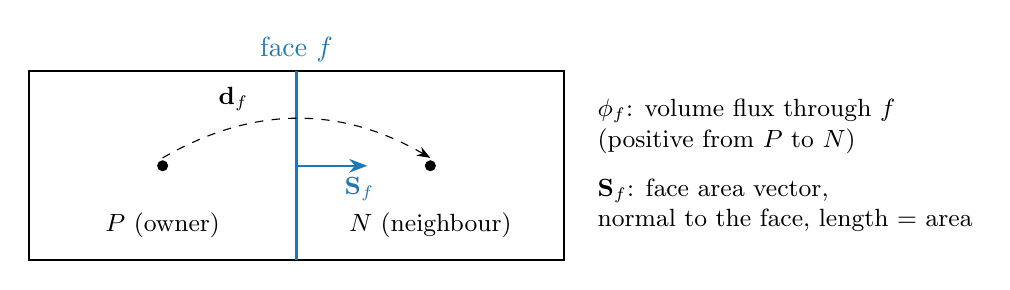
\begin{tikzpicture}[scale=1.0, >=Stealth]
  \draw[thick] (0,0) rectangle (3.4,2.4);
  \draw[thick] (3.4,0) rectangle (6.8,2.4);
  \fill (1.7,1.2) circle (2pt);
  \fill (5.1,1.2) circle (2pt);
  \node[font=\small] at (1.7,0.45) {$P$ (owner)};
  \node[font=\small] at (5.1,0.45) {$N$ (neighbour)};
  \draw[very thick, cfcoupled] (3.4,0) -- (3.4,2.4);
  \node[cfcoupled, above] at (3.4,2.4) {face $f$};
  \draw[->, thick, cfcoupled] (3.4,1.2) -- (4.3,1.2);
  \node[cfcoupled, font=\small] at (4.2,0.9) {$\vect{S}_f$};
  \draw[->, dashed] (1.7,1.3) to[bend left=30] (5.1,1.3);
  \node[font=\small] at (2.6,2.05) {$\vect d_f$};
  \node[font=\small, align=left, anchor=west] at (7.1,1.7)
    {$\phi_f$: volume flux through $f$\\ (positive from $P$ to $N$)};
  \node[font=\small, align=left, anchor=west] at (7.1,0.7)
    {$\vect S_f$: face area vector,\\ normal to the face, length = area};
\end{tikzpicture}
\caption{Two finite-volume cells sharing one face. Every balance in the
solver is a sum of face contributions like this one.}
\label{fig:fv}
\end{figure}

\begin{bblock}{finite volumes and faces}
\bbwhat The domain is split into cells; each conservation law becomes ``sum
of what flows through the faces of a cell $=$ sources in the cell''. Values
live at cell centres, fluxes live on faces.
\bbwhy Face fluxes shared by two cells are counted once as outflow of one
cell and once as inflow of the other, so mass is conserved exactly at the
discrete level, whatever the mesh looks like. This is what makes the
method robust on the unstructured \code{snappyHexMesh} meshes of real cars.
\bbwithout Every quantity that coupledFoam builds, from the matrix to the
Rhie--Chow flux, is a loop over faces. Nothing in this document works
without this picture.
\end{bblock}

After discretisation the equations of all cells together form a big system
of algebraic equations, one set of four equations per cell. Because each
cell only talks to its face neighbours, most entries of the corresponding
matrix are zero: the matrix is \emph{sparse}. OpenFOAM stores such a matrix
in its ``LDU'' format: a diagonal entry per cell and one ``upper'' and one
``lower'' entry per internal face.

\subsection{Residuals: how far from the answer?}\label{sec:residual}

A steady solver cannot compute the answer in one go, because the equations
are \emph{nonlinear}: the velocity convects itself, so the coefficients of
the equations depend on the solution. It iterates instead: guess, improve,
improve again. After every iteration one plugs the current fields into the
discrete equations and measures how badly they are violated. That
imbalance, cell by cell, is the \emph{residual}. At the exact discrete
solution it is zero.

coupledFoam summarises the residual in one number $R$: the size of the
imbalance of all four equations in all cells, normalised in the same way
OpenFOAM normalises its residuals, and divided by its value in the first
iteration. $R=10^{-6}$ therefore means ``the imbalance is a millionth of
what it was at the start''. For comparison with \code{simpleFoam}, the log
additionally prints $r_U$ and $r_p$, computed exactly like the ``Initial
residual'' that \code{simpleFoam} prints for $U$ and $p$
(D-016)\pro{Residual norms}.

\begin{pitfall}{residuals of different solvers are not directly comparable}
  $R$ of coupledFoam and the initial residuals of \code{simpleFoam} are
  normalised differently. A residual plot with both solvers shows the
  \emph{trend} of each, not which solver is ``more converged''. That is why
  all timing comparisons in this project use a solver-independent
  criterion: the force coefficients (or the pressure drop) must stop
  changing (Section~\ref{sec:protocol}).
\end{pitfall}

% =============================================================================
\section{The standard approach: SIMPLE and simpleFoam}\label{sec:simple}
% =============================================================================

\subsection{Guess and correct}

The workhorse of OpenFOAM for steady incompressible flow is
\code{simpleFoam}, based on the SIMPLE algorithm of Patankar and
Spalding~\cite{Patankar1972} or its variant SIMPLEC~\cite{VanDoormaal1984}.
It is \emph{segregated}: it never solves for velocity and pressure at the
same time. One SIMPLE iteration does the following
(Figure~\ref{fig:loops}, left):
\begin{enumerate}
\item Take the current pressure as if it were correct, and solve the three
  momentum equations for a new velocity.
\item This velocity generally violates continuity. Derive, from the
  continuity equation and a simplified form of the momentum equations, a
  \emph{pressure equation} (a Poisson-like equation) and solve it.
\item Correct the face fluxes and the velocity with the new pressure
  gradient, so that the fluxes conserve mass.
\item Blend the new values with the old ones (under-relaxation), solve the
  turbulence equations, and start again.
\end{enumerate}

\begin{figure}[tbp]
\centering
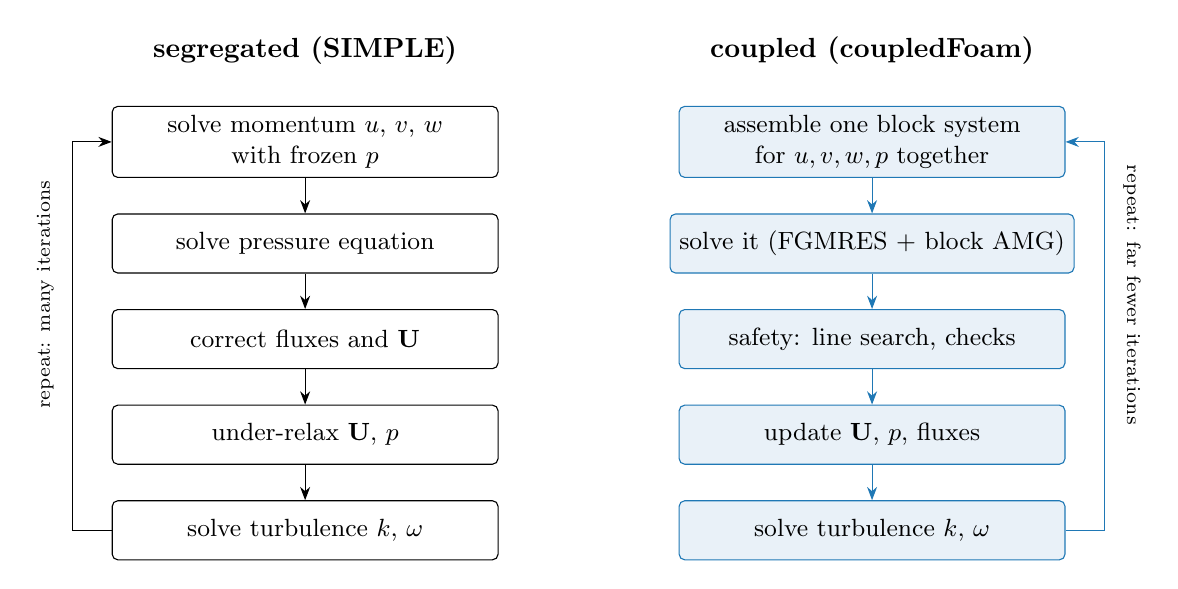
\begin{tikzpicture}[
  box/.style={draw, rounded corners=2pt, align=center, font=\small,
    minimum width=4.9cm, minimum height=0.75cm, fill=white},
  cbox/.style={box, fill=cfcoupled!10, draw=cfcoupled},
  >=Stealth, node distance=4.5mm]
  % segregated
  \node[font=\bfseries] (sT) at (0,0.2) {segregated (SIMPLE)};
  \node[box, below=4mm of sT] (s1) {solve momentum $u$, $v$, $w$\\ with frozen $p$};
  \node[box, below=of s1] (s2) {solve pressure equation};
  \node[box, below=of s2] (s3) {correct fluxes and $\Uv$};
  \node[box, below=of s3] (s4) {under-relax $\Uv$, $p$};
  \node[box, below=of s4] (s5) {solve turbulence $k$, $\omega$};
  \foreach \a/\b in {s1/s2,s2/s3,s3/s4,s4/s5} \draw[->] (\a) -- (\b);
  \draw[->] (s5.west) -- ++(-0.5,0) |- (s1.west);
  \node[font=\scriptsize, align=center, rotate=90] at (-3.3,-2.9)
    {repeat: many iterations};
  % coupled
  \node[font=\bfseries] (cT) at (7.2,0.2) {coupled (coupledFoam)};
  \node[cbox, below=4mm of cT] (c1) {assemble one block system\\ for $u,v,w,p$ together};
  \node[cbox, below=of c1] (c2) {solve it (FGMRES + block AMG)};
  \node[cbox, below=of c2] (c3) {safety: line search, checks};
  \node[cbox, below=of c3] (c4) {update $\Uv$, $p$, fluxes};
  \node[cbox, below=of c4] (c5) {solve turbulence $k$, $\omega$};
  \foreach \a/\b in {c1/c2,c2/c3,c3/c4,c4/c5} \draw[->, cfcoupled] (\a) -- (\b);
  \draw[->, cfcoupled] (c5.east) -- ++(0.5,0) |- (c1.east);
  \node[font=\scriptsize, align=center, rotate=-90] at (10.5,-2.9)
    {repeat: far fewer iterations};
\end{tikzpicture}
\caption{One outer iteration of the segregated SIMPLE algorithm (left) and
of the coupled solver (right). In SIMPLE, velocity and pressure take turns;
in coupledFoam they are solved together, and each iteration is more
expensive but achieves much more.}
\label{fig:loops}
\end{figure}

\subsection{Why SIMPLE needs under-relaxation}

In step 2 the pressure equation is derived from a \emph{simplified}
momentum equation: the influence of the neighbouring velocities is
neglected (SIMPLE) or approximated (SIMPLEC). The correction it produces is
therefore too large or pointed in a slightly wrong direction. Applied at
full strength it overshoots, the next iteration overshoots back, and the
run oscillates or diverges. The cure is \emph{under-relaxation}: accept
only a fraction of the change (for example 0.3 for pressure and 0.7 for
velocity in classical SIMPLE; SIMPLEC allows larger factors). The price is
that every iteration makes only a fraction of the progress it could make.

\begin{intuition}{two people at one shower}
  Imagine two people adjusting the same shower: one controls the hot tap
  (velocity), the other the cold tap (pressure). They take turns, and each
  only feels the water temperature after the other has already turned his
  tap. If both turn boldly, the temperature swings back and forth. If both
  turn only a little each time (under-relaxation), the temperature settles,
  but it takes many rounds. A coupled solver is one person with both hands
  on both taps.
\end{intuition}

\subsection{Why it takes so many iterations}

In the segregated loop, information between pressure and velocity is
exchanged only once per iteration, and only in relaxed doses. On a fine
mesh, a pressure disturbance also has to travel across many cells, and the
pressure equation is solved to a loose tolerance in each iteration. All
this makes each iteration cheap but the number of iterations large, and it
grows with the size of the mesh.

A concrete example from the test suite: on the lid-driven cavity at $Re=100$
(test T0, Section~\ref{sec:t0}), \code{simpleFoam} (SIMPLEC) needed
\cfnum{TZeroReOneZeroZeroNativeIterations} iterations to reach its residual
tolerance, while coupledFoam needed \cfnum{TZeroReOneZeroZeroIterations}.
(The two residuals are normalised differently, so this is an illustration of
the order of magnitude, not a race; see Section~\ref{sec:residual}.)

\begin{whyitmatters}{relaxation factors are case-specific}
  Users of \code{simpleFoam} usually spend time choosing relaxation
  factors: too small and the run crawls, too large and it diverges. The
  benchmark in this project therefore compares against two native settings:
  the tutorial's own, and a tuned SIMPLEC setting with factors 1.0 for $p$
  and 0.9 for $\Uv$, $k$, $\omega$ (Section~\ref{sec:protocol}).
  coupledFoam has no relaxation factors; its step size is controlled
  automatically by the pseudo-time step and the line search
  (Sections~\ref{sec:ptc} and~\ref{sec:ls}).
\end{whyitmatters}

% =============================================================================
\section{The coupled idea}\label{sec:coupled}
% =============================================================================

\subsection{Solve everything together}

A \emph{coupled} solver discretises the three momentum equations and the
continuity equation into \emph{one} linear system and solves for $u$, $v$,
$w$ and $p$ in all cells simultaneously. There is no pressure equation
derived from a simplified momentum equation, and hence no need to
under-relax the pressure: the pressure--velocity interaction is represented
exactly (for the current linearisation) inside the matrix. This approach
goes back to Vanka~\cite{Vanka1986} and was developed for unstructured
finite volumes by Darwish, Sraj and Moukalled~\cite{Darwish2007,Darwish2009}
and brought to OpenFOAM by Mangani, Buchmayr and
Darwish~\cite{Mangani2014a,Mangani2014b}. coupledFoam is a new,
independent implementation of this idea for OpenFOAM v2606.

\subsection{The \texorpdfstring{$4\times4$}{4x4} block structure}\label{sec:blocks44}

Because every cell has four unknowns $(u,v,w,p)$, the matrix is naturally
organised in small $4\times4$ \emph{blocks}: one block on the diagonal for
each cell (how the cell's four equations depend on its own four unknowns)
and one block for each face (how they depend on the neighbour's four
unknowns). Figure~\ref{fig:block} shows what is inside a block.

\begin{figure}[tbp]
\centering
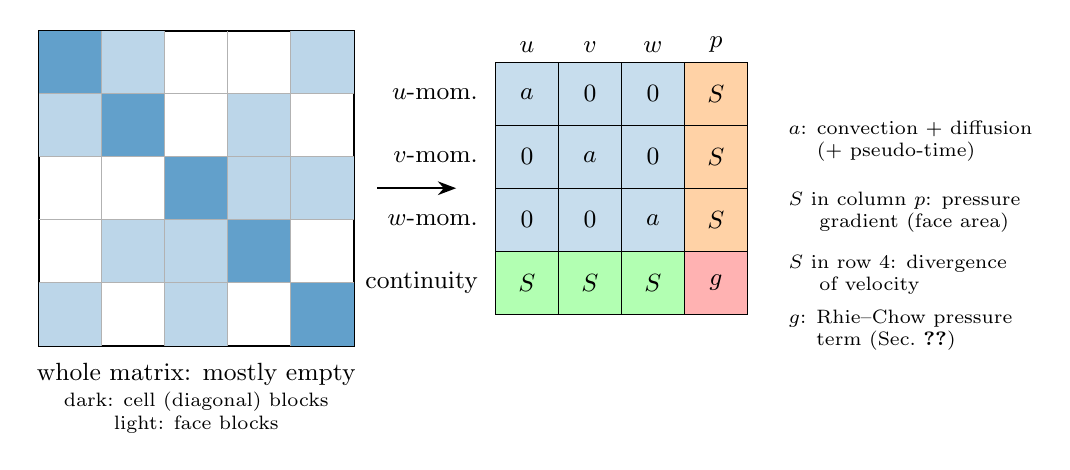
\begin{tikzpicture}[>=Stealth, font=\small]
  % big sparse matrix sketch
  \begin{scope}
    \draw[thick] (0,0) rectangle (4,4);
    \foreach \i in {0,...,4} {
      \fill[cfcoupled!70] (\i*0.8,4-\i*0.8-0.8) rectangle ++(0.8,0.8);
    }
    % face blocks (r,c) and (c,r): the pattern is symmetric
    \foreach \r/\c in {0/1,1/0,0/4,4/0,1/3,3/1,2/3,3/2,2/4,4/2} {
      \fill[cfcoupled!30] (\c*0.8,4-\r*0.8-0.8) rectangle ++(0.8,0.8);
    }
    \foreach \i in {1,...,4} {
      \draw[gray!60] (\i*0.8,0) -- (\i*0.8,4);
      \draw[gray!60] (0,\i*0.8) -- (4,\i*0.8);
    }
    \node[below] at (2,-0.1) {whole matrix: mostly empty};
    \node[align=center, font=\scriptsize] at (2,-0.85)
      {dark: cell (diagonal) blocks\\ light: face blocks};
  \end{scope}
  \draw[->, thick] (4.3,2.0) -- (5.3,2.0);
  % one block
  \begin{scope}[shift={(5.8,0.4)}]
    \def\s{0.8}
    \foreach \r in {0,...,3} \foreach \c in {0,...,3} {
      \draw (\c*\s, 3*\s-\r*\s) rectangle ++(\s,\s);
    }
    \fill[cfcoupled!25] (0,0.8) rectangle (2.4,3.2);
    \fill[orange!35] (2.4,0.8) rectangle (3.2,3.2);
    \fill[green!30] (0,0) rectangle (2.4,0.8);
    \fill[red!30] (2.4,0) rectangle (3.2,0.8);
    \foreach \r in {0,...,3} \foreach \c in {0,...,3} {
      \draw (\c*\s, 3*\s-\r*\s) rectangle ++(\s,\s);
    }
    \node at (0.4,2.8) {$a$}; \node at (1.2,2.0) {$a$}; \node at (2.0,1.2) {$a$};
    \node at (1.2,2.8) {$0$}; \node at (2.0,2.8) {$0$};
    \node at (0.4,2.0) {$0$}; \node at (2.0,2.0) {$0$};
    \node at (0.4,1.2) {$0$}; \node at (1.2,1.2) {$0$};
    \foreach \y in {2.8,2.0,1.2} \node at (2.8,\y) {$S$};
    \foreach \x in {0.4,1.2,2.0} \node at (\x,0.4) {$S$};
    \node at (2.8,0.4) {$g$};
    \node[anchor=east] at (-0.1,2.8) {$u$-mom.};
    \node[anchor=east] at (-0.1,2.0) {$v$-mom.};
    \node[anchor=east] at (-0.1,1.2) {$w$-mom.};
    \node[anchor=east] at (-0.1,0.4) {continuity};
    \node[above] at (0.4,3.2) {$u$}; \node[above] at (1.2,3.2) {$v$};
    \node[above] at (2.0,3.2) {$w$}; \node[above] at (2.8,3.2) {$p$};
  \end{scope}
  \node[align=left, anchor=west, font=\scriptsize] at (9.4,2.6)
    {$a$: convection + diffusion\\ \phantom{$a$: }(+ pseudo-time)};
  \node[align=left, anchor=west, font=\scriptsize] at (9.4,1.7)
    {$S$ in column $p$: pressure\\ \phantom{$S$: }gradient (face area)};
  \node[align=left, anchor=west, font=\scriptsize] at (9.4,0.9)
    {$S$ in row 4: divergence\\ \phantom{$S$: }of velocity};
  \node[align=left, anchor=west, font=\scriptsize] at (9.4,0.2)
    {$g$: Rhie--Chow pressure\\ \phantom{$g$: }term (Sec.~\ref{sec:rc})};
\end{tikzpicture}
\caption{Left: the coupled matrix is sparse; each small square is a
$4\times4$ block. Right: what a block contains. Rows 1--3 are the momentum
equations, row 4 is continuity; columns are the unknowns $u,v,w,p$. The
pressure column of the momentum rows (orange) and the velocity part of the
continuity row (green) are mirror images: the pressure gradient and the
velocity divergence are ``transposes'' of each other. The bottom-right entry
(red) exists only because of the Rhie--Chow interpolation. (In rotating MRF
zones the momentum part of the diagonal block also gets off-diagonal
entries, Section~\ref{sec:turb}.)}
\label{fig:block}
\end{figure}

Two things about this structure are worth remembering.

First, the bottom-right entry $g$ (``pressure--pressure'') would be
\emph{zero} in a naive discretisation, because the continuity equation does
not contain the pressure. A matrix with a zero block on the diagonal is
called a \emph{saddle-point} system; it is notoriously hard for iterative
solvers. The Rhie--Chow interpolation (Section~\ref{sec:rc}) is what fills
this entry and stabilises the system.

Second, each block holds 16 numbers, where a segregated solver stores one
number per cell and per face for each of its scalar equations. That is the
memory price of coupling; Section~\ref{sec:precision} explains how
coupledFoam reduces it by storing the blocks in single precision.

\subsection{Outer and inner iterations}

Even though velocity and pressure are solved together, coupledFoam still
iterates, because the equations are nonlinear. There are two nested loops,
and it helps to keep them apart:
\begin{itemize}
\item The \textbf{outer iteration} (also called nonlinear iteration): build
  the linear system from the current fields (convection uses the flux of
  the previous iteration), solve it, update the fields, update turbulence.
  This is the loop of Figure~\ref{fig:loops}, and the ``iterations'' in the
  log are outer iterations.
\item The \textbf{inner iteration} (linear solve): inside each outer
  iteration, the big linear system itself is solved iteratively, by a
  Krylov method with a multigrid preconditioner
  (Sections~\ref{sec:krylov}--\ref{sec:smoothers}). These are the ``linear
  iterations'' in the log.
\end{itemize}

\subsection{The trade-off, and the only fair comparison}\label{sec:fair}

A coupled outer iteration does much more than a SIMPLE iteration, so far
fewer of them are needed. But each one is more expensive: every coupling
between two cells is a $4\times4$ block of 16 numbers instead of the single
coefficients of SIMPLE's scalar equations, the system is harder to solve
than those separate scalar systems, and it needs more memory. Whether the coupled
solver is \emph{faster} in the end is therefore not obvious, and it can
depend on the case.

\begin{whyitmatters}{wall-clock time and CPU-hours, not iterations}
  An iteration count says nothing about the waiting time or the machine
  time used. A solver that needs 50 iterations of one minute each is
  slower than one that needs 2000 iterations of one second each. The
  project's explicit requirement (D-025) is therefore: the fastest solver
  wins, measured as
  \begin{itemize}
  \item \textbf{wall-clock time} to a converged answer (the waiting time),
    and
  \item \textbf{CPU-hours} to a converged answer (the computing time paid
    for: the CPU time of all ranks added up),
  \end{itemize}
  with the \emph{same} convergence criterion for both solvers. Iteration
  counts are shown only for completeness.
\end{whyitmatters}

\subsection{A map of one outer iteration}\label{sec:map}

Here is what coupledFoam does in every outer iteration, in plain words. Each
step points to the building block that explains it.
\begin{enumerate}
\item Decide, for every cell, how large a pseudo-time step it may take
  (Section~\ref{sec:ptc}).
\item Assemble the momentum rows, including the convection scheme via
  deferred correction (Section~\ref{sec:dc}) and the boundary conditions
  (Section~\ref{sec:bc}); limit the time step in cells where the step would
  change too much.
\item Assemble the continuity row with the Rhie--Chow flux
  (Section~\ref{sec:rc}); fix the pressure level in closed domains
  (Section~\ref{sec:pref}).
\item Compute the residual in double precision, store the matrix in single
  precision (Section~\ref{sec:precision}).
\item Solve the linear system for the \emph{change} of the fields with
  FGMRES and block multigrid (Sections~\ref{sec:krylov}--\ref{sec:smoothers}),
  to a tolerance chosen by Eisenstat--Walker (Section~\ref{sec:ew}).
\item Check the proposed change: line search, cut the CFL number and
  repeat if the step is too wild or the solve failed (Section~\ref{sec:ls}).
\item Apply the change (optionally accelerated by Anderson mixing,
  Section~\ref{sec:anderson}), update the face fluxes, check that nothing
  exploded, and roll back if it did (Section~\ref{sec:sentinel}).
\item Update the problem-cell sets (Section~\ref{sec:remediation}), solve
  the turbulence model (Section~\ref{sec:turb}), adapt the CFL number, write
  results and restart data (Section~\ref{sec:restart}), test for
  convergence.
\end{enumerate}

% =============================================================================
\section{The building blocks}\label{sec:blocks}
% =============================================================================

This section takes the solver apart. The order follows the map above:
first how the equations are built, then how the nonlinear iteration is kept
safe, then how the linear system is solved, and finally how single
precision is made to work.

% -----------------------------------------------------------------------------
\subsection{Boundary conditions and parallel interfaces}\label{sec:bc}

Every OpenFOAM boundary condition can express the boundary value as a
linear function of the adjacent cell value: ``boundary value $=$ (some
factor) $\times$ (cell value) $+$ (some constant)''. For a fixed value the
factor is zero; for zero gradient the factor is one and the constant zero.
OpenFOAM computes these two coefficients for every patch type anyway.
coupledFoam uses exactly these native coefficients to put every boundary
condition \emph{implicitly} into the block matrix (D-002). That is why
\code{fixedValue}, \code{zeroGradient}, \code{slip}, \code{symmetry},
\code{inletOutlet}, \code{totalPressure} and conditions derived from them
work without special code. For \code{inletOutlet} and \code{totalPressure},
the part that depends on the current flow direction or dynamic head is
taken from the previous outer iteration. Wall functions act, as usual,
through $\nu_t$ on the wall face.

When a case runs in parallel, the mesh is split into pieces
(\code{decomposePar}); the cut faces become \emph{processor} patches.
In coupledFoam these are treated fully implicitly: the matrix entries
across the cut are stored like any other face block and the neighbour
values are exchanged during every matrix--vector product. Periodic
(\code{cyclic}) and \code{cyclicAMI} patches are, in this version, coupled
\emph{explicitly}: the neighbour value from the previous outer iteration is
used as a known source. That works, but converges more slowly across such
patches; implicit coupling there is planned for Phase~2.

% -----------------------------------------------------------------------------
\subsection{Convection schemes and deferred correction}\label{sec:dc}

Convection (the flow carrying momentum along) needs the velocity on the
faces, but the unknowns live at cell centres. The simplest choice,
\emph{upwind}, takes the value of the upstream cell. It is very robust,
because it gives the matrix a strong diagonal, but it smears the solution
(numerical diffusion). Higher-order schemes such as \code{linearUpwind}
extrapolate from the upstream cell with its gradient; they are much more
accurate but make the matrix less well behaved.

coupledFoam uses the standard trick of \emph{deferred
correction}~\cite{Khosla1974,Ferziger2002}: the matrix always contains the
robust upwind operator, and the difference between the chosen scheme (from
\code{fvSchemes}, key \code{div(phi,U)}) and upwind is added as a known
source computed from the current fields. At convergence the source is exact,
so the converged solution is that of the chosen high-order scheme. A per-cell
blending factor $\beta$ between 0 (pure upwind) and 1 (full scheme) allows
switching the correction off locally.

\begin{bblock}{deferred correction and the upwind start-up}
\bbwhat Matrix $=$ upwind; right-hand side $=$ $\beta\times$(high-order
minus upwind), evaluated with the current fields.
\bbwhy It keeps the linear system easy to solve while delivering the
accuracy of the high-order scheme at convergence. For fresh runs, the first
50 iterations (or until $R<10^{-2}$) use pure upwind ($\beta=0$
everywhere), because the initial fields from \code{potentialFoam} are far
from the answer and a high-order correction would only add noise. Cells
with bad mesh quality or misbehaving values keep $\beta=0$
(Section~\ref{sec:remediation}).
\bbwithout Putting the high-order scheme directly into the matrix makes it
much harder for the smoother and the Krylov solver; dropping the correction
altogether gives an inaccurate, overly diffusive answer.
\end{bblock}

\begin{pitfall}{deferred correction at very large time steps}
  The correction is ``one step behind'', and the pseudo-time term
  (Section~\ref{sec:ptc}) is what damps this lag. As the CFL number becomes
  very large, that damping disappears. A simple analysis in the
  professional paper\pro{Deferred correction at high CFL} shows the iteration is still stable in
  idealised conditions, but with a small margin for high cell P\'eclet
  numbers. An inaccurate inner linear solve can use up that margin. This is
  part of the smoother story of Section~\ref{sec:smoothers}.
\end{pitfall}

% -----------------------------------------------------------------------------
\subsection{Rhie--Chow interpolation and the checkerboard problem}\label{sec:rc}

On a mesh where velocity and pressure are stored at the same place (cell
centres, as in OpenFOAM), a naive discretisation has a famous blind spot.
Consider the pressure along a row of cells alternating between high and low:
$100, 0, 100, 0, \dots$ (Figure~\ref{fig:checker}). The pressure gradient
in a cell is computed from the face values, which are averages of the two
neighbouring cells, so every face value is 50 and the gradient in every
cell is zero. The momentum equations do not feel this wildly oscillating
pressure at all, and nothing in the equations removes it. The resulting
solutions show a ``checkerboard'' pattern in the pressure.

\begin{figure}[tbp]
\centering
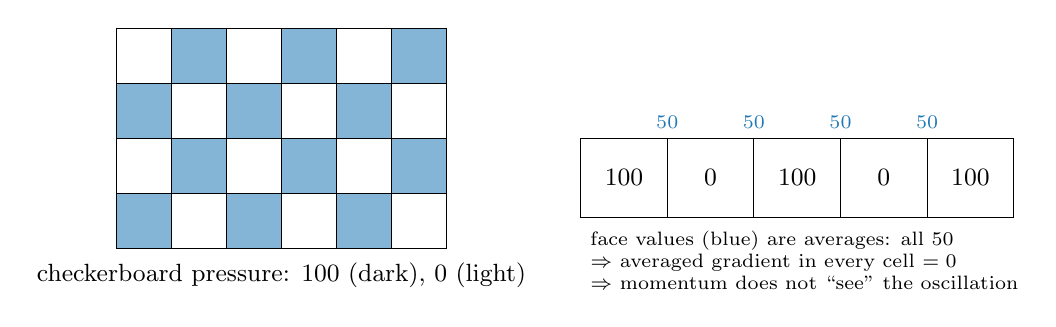
\begin{tikzpicture}[font=\small]
  \foreach \i in {0,...,5} \foreach \j in {0,...,3} {
    \pgfmathparse{mod(\i+\j,2)==0 ? "cfcoupled!55" : "white"}
    \edef\col{\pgfmathresult}
    \fill[\col] (\i*0.7,\j*0.7) rectangle ++(0.7,0.7);
    \draw (\i*0.7,\j*0.7) rectangle ++(0.7,0.7);
  }
  \node[below] at (2.1,-0.05) {checkerboard pressure: 100 (dark), 0 (light)};
  \begin{scope}[shift={(5.9,0.4)}]
    \foreach \i/\v in {0/100,1/0,2/100,3/0,4/100} {
      \draw (\i*1.1,0) rectangle ++(1.1,1.0);
      \node at (\i*1.1+0.55,0.5) {$\v$};
    }
    \foreach \i in {1,...,4} \node[cfcoupled, above] at (\i*1.1,1.0) {\scriptsize 50};
    \node[align=left, anchor=west, font=\scriptsize] at (0,-0.55)
      {face values (blue) are averages: all 50\\ $\Rightarrow$ averaged gradient in every cell $=0$\\
       $\Rightarrow$ momentum does not ``see'' the oscillation};
  \end{scope}
\end{tikzpicture}
\caption{The checkerboard problem. With cell-centred storage and averaged
face values, an alternating pressure field produces zero pressure force in
every cell. The Rhie--Chow term compares the direct difference across each
face ($100-0$) with the averaged gradient ($0$) and damps the mismatch.}
\label{fig:checker}
\end{figure}

Rhie and Chow~\cite{RhieChow1983} fixed this in the definition of the face
flux. The flux through a face is the interpolated velocity dotted with the
face area, \emph{plus} a correction proportional to
\begin{equation*}
  \underbrace{(p_N-p_P)\text{ measured directly across the face}}_{\text{sees the checkerboard}}
  \;-\;
  \underbrace{\text{average of the two cell pressure gradients}}_{\text{blind to it}} .
\end{equation*}
For a smooth pressure field the two terms are almost equal and the
correction is tiny; for a checkerboard they differ strongly, and the
correction creates a flux that drives the oscillation away. The size of the
correction is set by a coefficient $D=V/\bar a$ (cell volume over the
average momentum diagonal), which has the meaning ``how easily does the
velocity in this cell respond to a pressure difference''.

In coupledFoam the direct-difference part is implicit and appears in the
matrix as the pressure--pressure entry $g$ of Figure~\ref{fig:block}; the
averaged-gradient part is explicit. The continuity row \emph{is} the sum of
these Rhie--Chow fluxes over the faces of the cell, and after the solve the
new face fluxes are computed with \emph{exactly} the same face formula
(D-003)\pro{Continuity row and Rhie--Chow interpolation}. As a result, the mass imbalance of the fluxes that
coupledFoam writes out is exactly the continuity part of its residual, and
it vanishes as the solver converges.

\begin{bblock}{Rhie--Chow interpolation}
\bbwhat A correction of the face flux that compares the pressure difference
across a face with the interpolated cell pressure gradients.
\bbwhy It suppresses the checkerboard pressure mode and fills the empty
pressure--pressure block of the coupled system, turning an unsolvable
saddle point into a system that multigrid can handle.
\bbwithout Oscillating, meaningless pressure fields, and a linear system
with zeros on part of its diagonal that standard smoothers cannot even
start on.
\end{bblock}

On boundaries the Rhie--Chow term is only used where the pressure is fixed
(e.g.\ an outlet); on walls and velocity inlets it is switched off, since
it would otherwise create an artificial flux through the wall (D-013).

\begin{pitfall}{the pseudo-time step is inside $D$}
  $D=V/\bar a$ includes the pseudo-time term of the next section. The
  converged solution therefore depends slightly on the final local time
  step through the Rhie--Chow term, in the same way a SIMPLE solution
  depends slightly on its relaxation factor. At the large CFL numbers
  reached at convergence the effect is small, and the cavity comparison
  with \code{simpleFoam} (Section~\ref{sec:t0}) bounds it for that case.
\end{pitfall}

% -----------------------------------------------------------------------------
\subsection{Pseudo-transient continuation and the local CFL number}\label{sec:ptc}

The steady problem is solved as if it were a time-dependent problem that
is marched towards its steady state, but with a \emph{fake} (``pseudo'')
time step that is chosen for speed and robustness, not for accuracy. This
is called pseudo-transient continuation (PTC)~\cite{Kelley1998}.

Technically, every momentum equation gets an extra term $V/\Delta t$ on its
diagonal. A large diagonal makes the linear system easier to solve and
makes each step smaller and more cautious. Crucially, the solver computes
the \emph{change} of the fields in each iteration (``increment form'',
Section~\ref{sec:precision}), with the current fields as the ``old time''
values. The pseudo-time term then only enters the matrix, never the
residual: it controls \emph{how} the solver walks, but not \emph{where} it
ends up. The converged steady solution is the same whatever time steps were
used (up to the small Rhie--Chow effect noted above).

\begin{intuition}{walking down a foggy mountain}
  A walker descends into a valley in fog. Small steps are safe but slow;
  big steps are fast but risk a fall off a cliff. PTC is a rule for choosing
  the step length: start with small steps, and each time the ground has
  clearly gone downhill (the residual dropped), lengthen the stride. If a
  step looks dangerous, shorten it again. The valley floor (the steady
  solution) does not depend on the path taken.
\end{intuition}

\paragraph{Local time steps and the CFL number.}
The time step is not the same everywhere. Each cell gets its own $\Delta t$
from a \emph{CFL number}: roughly, the number of cells a fluid parcel would
cross in one time step. A small cell with fast flow gets a small $\Delta t$,
a large cell in slow flow a large one, so that all cells progress at a
similar ``speed'' towards the steady state. A diffusive limit is included
for regions where viscosity dominates. The global CFL number starts at 5
and is adapted automatically between 1 and 500 (defaults).

\paragraph{How the CFL number is adapted.}
The default strategy (``mRDM''~\cite{Ceze2011,Ceze2013AIAA}) looks at the
residual: if it went down, the CFL number is multiplied by the ratio of the
old to the new residual, at most by 1.5 per iteration; if it went up, the
CFL number is kept. The CFL number is \emph{reduced} only by the safety
mechanisms (line search, failed linear solves, rollbacks), and after every
reduction it is held for 10 iterations before it may grow again. Two
alternative strategies (EXP: fixed growth factor; SER~\cite{MulderVanLeer1985}:
proportional to the residual ratio, may also decrease) are selectable.

\paragraph{Solution-limited local time step.}
Even with a moderate global CFL number, a few cells (say, at a sharp edge)
may want to change much faster than the rest. Before the time step is
applied, coupledFoam estimates the change each cell would undergo; if it
exceeds half of the reference velocity, that cell's time step alone is
reduced. The global CFL can stay aggressive while individual trouble spots
are throttled.

\begin{bblock}{pseudo-transient continuation (PTC)}
\bbwhat A fake time step per cell, $V/\Delta t$ on the diagonal, steered by
an adaptive CFL number.
\bbwhy It is the coupled solver's replacement for under-relaxation: it
makes early iterations cautious and late iterations bold, automatically. It
also improves the linear system (larger diagonal) exactly when the flow is
still far from converged.
\bbwithout Solving the full steady coupled problem from a poor initial guess
in one Newton-like jump usually diverges. With a fixed small time step it
would be robust but as slow as a transient simulation.
\end{bblock}

\begin{whyitmatters}{reading the CFL column in the log}
  In a healthy run the CFL number climbs steadily towards its maximum and
  stays there. A CFL number that keeps dropping back, or never gets
  above a few tens, indicates that the solver is repeatedly running into
  trouble: look at the line-search factor, the cut counter and the
  remediation set sizes in the same log line.
\end{whyitmatters}

% -----------------------------------------------------------------------------
\subsection{Line search and physicality checks}\label{sec:ls}

The linear solve proposes a change $\delta\Uv$, $\delta p$ for every cell.
Before it is applied, coupledFoam asks: \emph{is this change physically
reasonable?} The rule~\cite{Ceze2013AIAA} is simple: no cell's velocity may
change by more than 30\,\% of a reference velocity $U_{\mathrm{ref}}$ (the
largest velocity in the domain at the first iteration), and no cell's
pressure by more than half the reference dynamic pressure
$p_{\mathrm{ref}}=\tfrac12U_{\mathrm{ref}}^2$. If the proposed change is too
large somewhere, the \emph{whole} change is scaled down by a factor
$\omega\le1$ (the line-search factor) until the rule holds.

If $\omega$ would have to be smaller than 0.1, the step is considered bad:
the CFL number is halved and the step is recomputed from the same fields,
up to three times. If it is still bad, the step is taken with $\omega=0.1$,
and the cells that caused the problem are marked for special treatment
(Section~\ref{sec:remediation}).

A linear solve that failed (did not reduce its residual or produced
non-finite numbers) is treated the same way: CFL cut and repeat (D-020,
D-029). After three consecutive failed linear solves the run stops with a
diagnostic output rather than carrying on with garbage.

\begin{bblock}{line search}
\bbwhat A factor $\omega\in(0,1]$ that shortens the proposed update so that
no cell changes by more than a fixed fraction of the reference velocity or
pressure.
\bbwhy The linear system is only a local approximation of the nonlinear
problem; far from convergence its answer can be wildly wrong in a few
cells. The line search keeps such a step from wrecking the fields.
\bbwithout One bad step in a single cell (e.g.\ at a sharp corner) could
create huge velocities, negative turbulence quantities, and a diverged run.
\end{bblock}

\begin{pitfall}{a failed solve must not be applied at all}
  During development a linear solve near the single-precision floor
  diverged, and the original rule ``after the cuts, accept the step with
  $\omega=0.1$'' applied 10\,\% of a garbage increment to an already
  converged solution and destroyed it (D-020). Since then a failed solve is
  never applied, and the Krylov solvers return their best iterate rather
  than their last one.
\end{pitfall}

\begin{whyitmatters}{what $\omega$ in the log indicates}
  $\omega=1$ means the full step was taken. Values well below one in the
  early iterations are normal. Persistent small $\omega$ late in the run
  means some region keeps producing large changes; the dynamic remediation
  set size (next section) gives the number of cells involved.
\end{whyitmatters}

% -----------------------------------------------------------------------------
\subsection{Remediation: special treatment for problem cells}\label{sec:remediation}

Real meshes of real cars contain a few bad cells: highly non-orthogonal,
skewed, stretched, or next to a much larger neighbour. And during a run,
some cells may temporarily misbehave. coupledFoam handles both with
\emph{cell sets} that get gentler numerics locally, instead of making the
whole simulation more cautious.

\begin{description}
\item[Static set (chosen in advance).] Built once before the first
  iteration, in four categories that can each be switched on or off and
  tuned in the case files (D-066):
  \emph{meshQuality} (faces too non-orthogonal or skewed, a large volume
  jump to a neighbour, or very stretched cells), \emph{badMesh} (severe
  defects such as a neighbour more than 50 times larger, or cells whose
  faces do not close), \emph{processor} (cells at the boundaries between
  the parts of a parallel run) and \emph{wall} (optionally, cells next to
  chosen walls). The defective cells of the first two categories get pure
  upwind convection, a stronger limiter on the non-orthogonal correction,
  a limited pressure gradient in the Rhie--Chow term, and half the time
  step. The processor and wall cells are chosen by where they are, not
  because they are bad; they only get half the time step and keep the
  accurate convection scheme. Giving a dozen well-shaped cells on the
  motorbike body the full treatment changed the lift by 18\,\% (D-061).
\item[Dynamic set (bad behaviour).] Updated every iteration. A cell is
  added if its velocity exceeds four times the reference, its pressure
  exceeds 15 times the reference (D-044), it differs strongly from its
  neighbours, any
  value is not a finite number, or the line search or the rollback
  (Section~\ref{sec:sentinel}) points at it. The cell and its direct
  neighbours then get pure upwind, a tenth of the time step, and a clip on
  how far the update may move them away from their neighbours' mean. A cell
  leaves the set after 20 quiet iterations. A warning appears if the sets
  cover more than 1\,\% of the mesh.
\item[Zonal factors (optional).] Cell zones or patches (with a number of
  cell layers around them) can be named in which the time step and the
  high-order blending are reduced, e.g.\ around a wheel. Off by
  default (D-027).
\end{description}

\begin{intuition}{local speed limits}
  Rather than lowering the speed limit on the whole motorway because of one
  construction site, a local limit is posted at the construction site.
  Remediation is exactly that: local time step and scheme reductions where
  they are needed, full speed everywhere else.
\end{intuition}

\begin{whyitmatters}{what the remediation sets mean for accuracy}
  Pure upwind in a handful of cells changes the solution only locally and
  slightly. The test criteria require the static set to stay at or below
  1\,\% of the cells on the motorBike meshes (T4), and an empty dynamic set
  at convergence on the airfoil (T3). If a large fraction of the cells of
  a case ends up in the sets, that is a sign to improve the mesh.
\end{whyitmatters}

% -----------------------------------------------------------------------------
\subsection{Sentinel and rollback}\label{sec:sentinel}

Before every field update, coupledFoam keeps a copy of the fields. After
the update (and again after the turbulence update), a ``sentinel'' checks
three things: are all values finite numbers, is the largest velocity below
10 times the reference, and is the largest pressure below 50 times the
reference? If not, the copy is restored (a \emph{rollback}), the CFL number
is cut to a quarter, and the offending cells go into the dynamic set. After
five consecutive rollbacks the run stops, writes the last valid fields into
a time directory \code{<iteration>\_lastValid} together with a field that
marks the offending cells, prints their positions, and exits with an error.
A time directory containing \code{nan} or \code{inf} is never written.

\begin{whyitmatters}{when a run stops}
  If coupledFoam stops with a sentinel error, open the \code{\_lastValid}
  time directory in ParaView and look at the \code{sentinelFlag} field: it
  shows where the trouble started, usually at a mesh defect or a
  boundary-condition problem.
\end{whyitmatters}

% -----------------------------------------------------------------------------
\subsection{Restart}\label{sec:restart}

Whenever results are written, coupledFoam writes the normal OpenFOAM fields
and, last, a small dictionary \code{coupledState} with everything the
iteration needs to continue exactly where it stopped: iteration number, CFL
number, residual history values, reference values, the dynamic set, the
rollback counters and more (D-017). It is written under a temporary name and
renamed at the end, so its presence guarantees that the time directory is
complete. On restart, the face fluxes are recomputed from the stored
velocity and pressure with the stored Rhie--Chow coefficient, and the
difference to the stored fluxes is logged as a consistency check. The
restart test (T-restart) requires that a run split in two reaches the same
answer as a continuous run. The optional Anderson history
(Section~\ref{sec:anderson}) is not part of the restart state (D-026): a
restarted run begins with an empty history.

% -----------------------------------------------------------------------------
\subsection{Krylov solvers: GMRES, FGMRES and BiCGStab}\label{sec:krylov}

Now to the inner loop: solving the big linear system $\mathsf A\,\vect x=\vect b$
once per outer iteration. For millions of cells a direct solution
(Gaussian elimination) is out of the question in memory and time. Iterative
\emph{Krylov} methods~\cite{Saad2003} are used instead.

\begin{intuition}{building the answer from repeated experiments}
  A Krylov method only needs one operation: ``multiply a vector by the
  matrix''. It starts with the current error (the residual), multiplies it
  by the matrix, multiplies the result again, and so on. Each product shows
  how the system ``responds'' to a certain pattern. From these responses it
  builds a combination that best explains the right-hand side. A
  comparison is the tuning of a sound system: a few test signals are played, the response of
  the room is recorded, and they are combined into the correction that best
  cancels the echo.
\end{intuition}

\begin{description}
\item[GMRES] (Generalised Minimal RESidual) keeps all the directions it has
  generated and picks, at every step, the combination with the smallest
  residual. It never gets worse, but the memory grows with every step, so
  it is \emph{restarted} after $m$ steps (default $m=10$; $m=6$ above 40
  million cells to save memory).
\item[FGMRES] (Flexible GMRES~\cite{Saad1993}) is GMRES that additionally
  stores the preconditioned directions. This costs twice the memory but
  allows the preconditioner to be slightly different every time it is
  applied, which is the case for the K-cycle multigrid
  (Section~\ref{sec:amg}). FGMRES is the default in coupledFoam, and the
  K-cycle is refused at start-up with any other Krylov solver.
\item[BiCGStab] (BiConjugate Gradient Stabilised) needs only a few vectors
  regardless of the number of steps, but its residual does not decrease
  monotonically and it can break down. coupledFoam's version restarts
  after a breakdown and returns the best iterate it has seen.
\end{description}

All inner products and norms inside these solvers are accumulated in double
precision, even though the vectors are stored in single precision
(Section~\ref{sec:precision}).

\begin{bblock}{Krylov solver}
\bbwhat An iterative method that improves the solution of
$\mathsf A\vect x=\vect b$ using only matrix--vector products and
combinations of vectors.
\bbwhy It is the only affordable way to solve linear systems with tens of
millions of unknowns, and it parallelises well.
\bbwithout Direct solvers would need far more memory than the machine has
for any realistic mesh.
\end{bblock}

% -----------------------------------------------------------------------------
\subsection{Preconditioning}\label{sec:precond}

On its own, a Krylov method converges slowly on the coupled system: the
matrix mixes scales from single cells to the whole domain, and a handful of
matrix--vector products cannot capture that. A \emph{preconditioner} $\mathsf M$
is a cheap, approximate inverse of $\mathsf A$. Instead of the original
system, the Krylov method solves one in which $\mathsf A$ is combined with
$\mathsf M^{-1}$; if $\mathsf M$ is a good approximation, this combined
system is close to the identity and is solved in a few steps.

\begin{intuition}{glasses for the solver}
  The Krylov method is a good reader with bad eyes. The preconditioner is a
  pair of glasses: it does not do the reading, but it makes the text sharp
  enough that reading is fast. Better glasses (a stronger preconditioner)
  cost more to make, so there is a sweet spot.
\end{intuition}

coupledFoam offers two preconditioners: \code{blockDiagonal} (invert only
the $4\times4$ diagonal block of each cell; cheap and weak; used in the
benchmark to measure how much the multigrid is worth) and \code{blockGAMG},
the block algebraic multigrid described next (the default).

% -----------------------------------------------------------------------------
\subsection{Algebraic multigrid}\label{sec:amg}

\paragraph{The key observation.} Simple iterative ``smoothers'' such as
Gauss--Seidel (Section~\ref{sec:smoothers}) update each cell from its
neighbours. They remove \emph{jagged} errors (errors that change sign from
cell to cell) very quickly, because those are local. But \emph{smooth}
errors, spread over hundreds of cells, are reduced only very slowly:
information travels one cell per sweep.

\paragraph{The key trick.} A smooth error on a fine mesh looks jagged on a
much coarser mesh. So: smooth a little on the fine mesh, then transfer the
remaining (smooth) error problem to a coarser mesh, where it is cheap to
reduce, and recursively to even coarser meshes; then interpolate the
correction back and smooth again. That is \emph{multigrid}.

\begin{intuition}{fixing a picture at several zoom levels}
  The colour balance of a large photo is not repaired pixel by pixel: the
  overall tone is fixed on a thumbnail, then the regional shading at medium
  size, then the fine details at full size. Each level
  corrects the errors it can see best.
\end{intuition}

\paragraph{Algebraic and additive-correction.} OpenFOAM's \code{GAMG} and
coupledFoam's \code{blockGAMG} build the coarse ``meshes'' purely from the
matrix and the geometry of the faces, without a second mesh file:
neighbouring cells are glued together into coarse cells
(\emph{agglomeration}), using OpenFOAM's own \code{faceAreaPair}
agglomeration. In the additive-correction
approach~\cite{Hutchinson1986,Weiss1999}, the equation of a coarse cell is
simply the sum of the equations of its fine cells, and the coarse
correction is added unchanged to all fine cells it contains. coupledFoam
does this with $4\times4$ blocks; the sums are accumulated in double
precision and the result is stored in single precision. With
\code{mergeLevels 2}, two pairwise agglomeration steps are merged into one
level, so each level has roughly a quarter of the cells of the one above.

\begin{figure}[tbp]
\centering
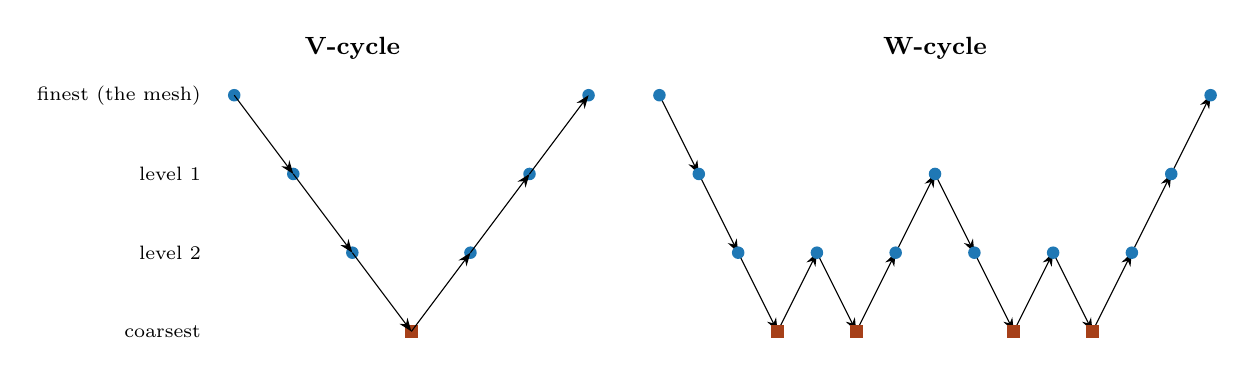
\begin{tikzpicture}[>=Stealth, font=\small,
  lev/.style={circle, fill=cfcoupled, inner sep=1.6pt},
  crs/.style={rectangle, fill=cfpit, inner sep=2.4pt}]
  % V-cycle
  \begin{scope}
    \node at (1.5,0.6) {\textbf{V-cycle}};
    \foreach \x/\y in {0/0,0.75/-1,1.5/-2} \node[lev] (v\x) at (\x,\y) {};
    \node[crs] at (2.25,-3) {};
    \foreach \x/\y in {3/-2,3.75/-1,4.5/0} \node[lev] at (\x,\y) {};
    \draw[->] (0,0) -- (0.75,-1); \draw[->] (0.75,-1) -- (1.5,-2);
    \draw[->] (1.5,-2) -- (2.25,-3); \draw[->] (2.25,-3) -- (3,-2);
    \draw[->] (3,-2) -- (3.75,-1); \draw[->] (3.75,-1) -- (4.5,0);
  \end{scope}
  % W-cycle
  \begin{scope}[shift={(5.4,0)}]
    \node at (3.5,0.6) {\textbf{W-cycle}};
    \coordinate (a) at (0,0); \coordinate (b) at (0.5,-1);
    \coordinate (c) at (1.0,-2); \coordinate (d) at (1.5,-3);
    \coordinate (e) at (2.0,-2); \coordinate (f) at (2.5,-3);
    \coordinate (g) at (3.0,-2); \coordinate (h) at (3.5,-1);
    \coordinate (i) at (4.0,-2); \coordinate (j) at (4.5,-3);
    \coordinate (k) at (5.0,-2); \coordinate (l) at (5.5,-3);
    \coordinate (m) at (6.0,-2); \coordinate (n) at (6.5,-1);
    \coordinate (o) at (7.0,0);
    \draw[->] (a)--(b); \draw[->] (b)--(c); \draw[->] (c)--(d); \draw[->] (d)--(e);
    \draw[->] (e)--(f); \draw[->] (f)--(g); \draw[->] (g)--(h); \draw[->] (h)--(i);
    \draw[->] (i)--(j); \draw[->] (j)--(k); \draw[->] (k)--(l); \draw[->] (l)--(m);
    \draw[->] (m)--(n); \draw[->] (n)--(o);
    \foreach \p in {a,b,c,e,g,h,i,k,m,n,o} \node[lev] at (\p) {};
    \foreach \p in {d,f,j,l} \node[crs] at (\p) {};
  \end{scope}
  % labels
  \foreach \y/\t in {0/finest (the mesh),-1/level 1,-2/level 2,-3/coarsest} {
    \node[anchor=east, font=\scriptsize] at (-0.3,\y) {\t};
  }
\end{tikzpicture}
\caption{Multigrid cycles over four levels. Going down: smooth, then pass
the remaining residual to the coarser level. Going up: add the coarse
correction, smooth again. Blue dots: smoothing; orange squares:
coarsest-level solve. The V-cycle visits each coarse level once; the
W-cycle visits coarse levels repeatedly, which is stronger but more
expensive. The F-cycle lies in between; the K-cycle decides at every level
and every visit whether a second, W-like visit is worth it.}
\label{fig:vcycle}
\end{figure}

\paragraph{Cycle types.} How often the coarse levels are visited is the
\emph{cycle type} (Figure~\ref{fig:vcycle}):
\begin{description}
\item[V] once per level: cheapest.
\item[W] twice per level, recursively: strongest and most expensive.
\item[F] in between: one extra visit per level.
\item[K] (Notay and Vassilevski~\cite{NotayVassilevski2008}, the basis of
  the AGMG solver~\cite{Notay2010}; default): at each coarse level, the
  correction is treated as a mini-Krylov step; if the first visit reduced
  the coarse residual well (to a quarter or better), it stops there
  (V-like); otherwise it makes a second visit and optimally combines the
  two (W-like). It thus adapts per level and per application.
\end{description}
Additive-correction multigrid has a comparatively weak coarse-level
correction, which is why a plain V-cycle does not scale optimally with it,
and why the adaptive K-cycle was designed as the default. The measurements
on systems dumped from T1--T4 later showed the V-cycle with a damped ILU(0)
smoother to be the more robust choice on the project's meshes, and it is
the default since D-043; the K-cycle remains available. Because the K-cycle is not
exactly the same operation every time it is applied, it needs the flexible
Krylov solver FGMRES.

\paragraph{What cycles cost.} If each level has $r$ times fewer cells than
the one above, the work of one cycle, measured in units of ``one sweep on
the finest mesh'', is (derived in the professional paper\pro{Block additive-correction AMG}):
\begin{center}\small
\begin{tabular}{lrrrr}
\toprule
coarsening ratio $r$ & 2 & 3 & 4 & 8\\
\midrule
V & 2.00 & 1.50 & 1.33 & 1.14\\
F & 4.00 & 2.25 & 1.78 & 1.31\\
W & $\infty$ & 3.00 & 2.00 & 1.33\\
\bottomrule
\end{tabular}
\end{center}
With plain pairwise agglomeration ($r=2$) a W-cycle would cost more with
every additional level. The solver therefore enforces a rule: for W- and
K-cycles every level must have at least three times fewer cells than the
one above; if not, it merges more agglomeration steps (up to four) and
tries again, and stops with an error if the rule still fails. It also
checks that the total size of all coarse matrices stays below 1.5 times the
fine matrix (``operator complexity'').

\paragraph{The coarsest level.} At the bottom of the hierarchy the system is
small. If it has at most 64 cells on one rank, it is solved exactly by a
dense LU factorisation in double precision; otherwise by a few BiCGStab
iterations. The choice is automatic and printed in the log.

\begin{bblock}{algebraic multigrid (block-GAMG)}
\bbwhat A hierarchy of ever coarser versions of the matrix, built by gluing
cells together, with smoothing on each level and corrections passed
between levels.
\bbwhy It reduces errors of all sizes at a cost proportional to the number
of cells. It is what makes the solver usable on meshes with millions of
cells.
\bbwithout With a simple preconditioner (block diagonal), the number of
Krylov iterations grows strongly with mesh size; configuration D of the
benchmark measures exactly this (Section~\ref{sec:protocol}).
\end{bblock}

\paragraph{Cycle-efficiency controller (autoTune).} The solver measures
how well the multigrid cycle works: on the first application in each
linear solve it checks by how much one cycle reduces the residual (the
ratio $\rho$; small is good). Every 50 outer iterations it looks at the
median $\rho$. If the cycle is weak ($\rho>0.7$ in two consecutive windows)
it adds post-smoothing sweeps (up to 4) and, for V and F cycles, promotes
the cycle type (V$\to$F$\to$W, only if the coarsening rule allows); if the
cycle is very effective ($\rho<0.3$) it removes sweeps again. Changes happen
only between linear solves and are logged as events. The K-cycle is not
promoted further, since it adapts internally.

% -----------------------------------------------------------------------------
\subsection{Smoothers: why Gauss--Seidel failed and ILU(0) worked}\label{sec:smoothers}

The smoother is the local workhorse of each multigrid level. coupledFoam
has two:
\begin{description}
\item[Block Gauss--Seidel.] Go through the cells one by one; for each cell,
  solve its own $4\times4$ block exactly, using the latest values of the
  neighbours. Cheap and simple.
\item[Block ILU(0)] (incomplete LU factorisation without fill-in, in
  OpenFOAM's ``DILU'' form, D-015). Build an approximate factorisation of
  the whole matrix that keeps the original sparsity pattern and only
  modifies the diagonal blocks, then apply it in one forward and one
  backward sweep. More expensive to set up, but it transports information
  along the whole sweep direction and treats the coupling between cells
  much more faithfully.
\end{description}

\paragraph{A learning story (D-028).} During development, the cavity at
$Re=1000$ with the \code{linearUpwind} scheme refused to converge with
the original configuration (BiCGStab, block multigrid, block Gauss--Seidel
smoother): as soon as the upwind start-up ended and deferred correction
was switched on, the CFL number oscillated, the line search kept cutting
it, and the residual stagnated far above the target. With pure upwind the
same configuration converged. The obvious suspect was deferred correction
at large time steps, and an analysis (Section~\ref{sec:dc}, pitfall box)
showed that the theoretical stability margin is indeed small.

The decisive experiment was different: \emph{keep everything the same and
only change the smoother to block ILU(0)}. The same discretisation then
reached the maximum CFL number without a single cut and converged to
$R<10^{-8}$ quickly, with a fraction of the Krylov iterations and of the
solve time. The real culprit was the \emph{quality of the inner solve}:
the $4\times4$ point smoother is weak on the saddle-point structure of the
coupled system, the resulting poor increments were what made the outer
iteration oscillate, and deferred correction merely had too little margin
to absorb them. The measured details are in D-028 and in the professional
paper\pro{Deferred correction at high CFL}.

\begin{whyitmatters}{what this story teaches}
  \begin{itemize}
  \item Symptoms in the outer iteration (oscillating CFL, stagnating
    residual) can be caused by the inner linear solver. Before changing
    the discretisation, check whether the linear solves reach their
    tolerance.
  \item The accuracy of the inner solve and the robustness of the outer
    iteration have to be designed together. This is why coupledFoam has
    the Eisenstat--Walker tolerance (Section~\ref{sec:ew}), stronger
    cycles, and the treatment of failed solves.
  \end{itemize}
\end{whyitmatters}

\paragraph{Current status of the default.} The formal decision on the
default smoother is made by a dedicated benchmark on the backward-facing
step (T2, gate B2 of the specification: ILU(0) must bring at least 15\,\%
wall-clock gain). Until that is run, the test cases still name
\code{blockGaussSeidel}; the recommended settings for the F1 case
(Section~\ref{sec:f1}) already use \code{blockILU0}.

% -----------------------------------------------------------------------------
\subsection{Eisenstat--Walker: do not over-solve}\label{sec:ew}

How accurately should the linear system be solved in each outer iteration?
Early on, the matrix itself is only a rough approximation of the nonlinear
problem (it was built from fields that are still far from the answer).
Solving it to ten digits is wasted effort: the next outer iteration builds
a different matrix anyway. Late in the run, when the outer iteration
converges fast, a sloppy linear solve would slow it down.

The Eisenstat--Walker rule~\cite{EisenstatWalker1996,Knoll2004} sets the
linear tolerance $\eta_n$ (the factor by which the linear residual must be
reduced) from the progress of the outer iteration: roughly $\eta_n\approx
0.9\,(R_n/R_{n-1})^2$. When the outer residual drops quickly, $\eta_n$
becomes small (solve more accurately); when it stagnates, $\eta_n$ stays
large (solve loosely). It is kept between $10^{-3}$ and $0.5$, is $0.5$ in
the first iteration and during the upwind start-up, and at least one
Krylov iteration is always made.

\begin{intuition}{measuring with the right ruler}
  A board sawn roughly to length is not measured with a micrometer;
  millimetre precision is needed only for the final cut.
  Eisenstat--Walker picks the measuring precision of each inner solve to
  match how close the outer iteration is to the answer.
\end{intuition}

\begin{pitfall}{a zero increment freezes the solver}
  If the linear solver's absolute tolerance is reached before the outer
  target, the solver may decide to do zero iterations, the increment is
  zero, and the outer iteration stops moving. This happened on the cavity
  (D-022). Hence the rule ``at least one Krylov iteration'', and the
  requirement that the absolute linear tolerance lie below the outer
  target.
\end{pitfall}

% -----------------------------------------------------------------------------
\subsection{Anderson acceleration (optional)}\label{sec:anderson}

Anderson acceleration~\cite{Anderson1965,WalkerNi2011} looks at the last
few outer updates (default four) and asks: is there a combination of them
that would have predicted the current one better? If the updates follow a
pattern (for example, they keep zig-zagging), it extrapolates along that
pattern and takes a larger, better-aimed step. The extrapolated state must
pass the same sentinel checks; the history is cleared after every CFL cut,
every change of the remediation sets and every rollback.

It is \emph{off by default}, because it needs to store the recent history:
about 320 bytes per cell for four steps, which matters at tens of millions
of cells. The benchmark measures whether it pays off on T1 and T3
(Figure~\ref{fig:anderson}).

% -----------------------------------------------------------------------------
\subsection{Processor agglomeration: gathering coarse levels}\label{sec:procagg}

In a parallel run each rank owns a piece of the mesh. On the fine levels
each rank has plenty of work, but a few levels down each rank owns only a
handful of coarse cells, and the time is dominated by waiting for messages
from other ranks (\emph{latency}), not by arithmetic. coupledFoam therefore
gathers coarse levels onto fewer ranks: a level with fewer than 5000 cells
per rank is moved onto a quarter of the ranks, and a level with fewer than
5000 cells in total onto one rank (D-030). The finest level is never
gathered.

\begin{intuition}{do not hold a ten-person meeting about three items}
  If ten people each have one small item to decide, calling a meeting where
  everyone waits for everyone else costs more than letting one person
  collect the items and decide alone. Skipping the coarse levels altogether
  is not an option: they carry the large-scale correction and cost less
  than 5\,\% of the cycle work.
\end{intuition}

% -----------------------------------------------------------------------------
\subsection{Float versus double: the precision design}\label{sec:precision}

Computers store real numbers in \emph{floating point}: double precision
(``double'', 8 bytes, about 16 significant digits) or single precision
(``float'', 4 bytes, about 7 digits). OpenFOAM normally works entirely in
double.

\paragraph{Why float at all?} Sparse linear algebra is limited by
\emph{memory bandwidth}: the processor spends most of its time waiting for
matrix entries to arrive from memory, not computing with them. A float
matrix is half the size, so it can be streamed through the processor in
roughly half the time. The coupled matrix
needs 16 numbers per cell for the diagonal block and 32 per internal face
for the two off-diagonal blocks; on a hexahedral mesh with about three
internal faces per cell that is about 448 bytes per cell in float, half the
double-precision figure. Memory size matters just as much: the budget for
the largest target mesh (45 million cells) is set out in the professional
paper\pro{Storage and precision}.

\paragraph{Why not float everywhere?} Seven digits are not enough to add up
millions of numbers accurately, and not enough to reach the residual levels
a converged steady solution needs. So coupledFoam separates two roles
(D-001, D-012):
\begin{itemize}
\item \textbf{Stored in float} (\code{blockScalar}): the block matrix and all
  Krylov and multigrid vectors, i.e.\ the big, bandwidth-hungry data.
\item \textbf{Computed in double} (\code{reduceScalar}): every sum, dot
  product and norm (accumulated in double, reduced across ranks in double),
  the Galerkin sums of the coarse levels, the small dense matrices of
  GMRES, and above all \emph{the residual $\vect b-\mathsf A\vect x$}, which is
  computed from the double-precision assembly before the matrix is rounded
  to float.
\end{itemize}

\paragraph{Why this works: the increment form.} In each outer iteration the
solver does not solve for the new fields, but for the \emph{change}
$\delta\vect x$: $\mathsf A_{\text{float}}\,\delta\vect x\approx\vect r$, with
the residual $\vect r$ computed in double. The float solve only has to get
the change roughly right; the next iteration measures the remaining error
exactly again, in double, and corrects it. The final accuracy is therefore
set by the double-precision residual, not by the float solve. This is the
classical idea of mixed-precision iterative
refinement~\cite{Baboulin2009,Carson2018}, built into the outer iteration.

\begin{intuition}{a cheap tape measure and a precise reference}
  A machine part is adjusted with a cheap tape measure (the float solve)
  and checked after each adjustment against a precise gauge (the double
  residual). The cheap tape is good enough to tell which way and roughly how
  far to adjust; the precise gauge guarantees that the work does not stop
  until the part is exactly right.
\end{intuition}

\begin{pitfall}{why OpenFOAM's own mixed-precision build did not help}
  The specification asked for OpenFOAM's \code{SPDP} build. It turned out
  that in OpenFOAM v2606 this build does the opposite of what is needed:
  it stores the \emph{fields} in float and \emph{solves} in double (D-001).
  coupledFoam therefore runs on a normal double-precision OpenFOAM and
  defines its own float and double types for the block data. The native
  \code{simpleFoam} reference thus uses the same double-precision fields.
\end{pitfall}

\begin{pitfall}{adding many small numbers in float}
  Summing $10^8$ copies of $10^{-4}$ in float gives a visibly wrong result,
  because each small addition to a large running sum is rounded away. The
  unit test \code{Test-doubleReduce} demonstrates this and checks that the
  double accumulator is exact (D-004). Every reduction in the solver
  therefore goes through the double-precision layer.
\end{pitfall}

Other safety measures of the precision design: the $4\times4$ block
inversions are done in double with a guard against zero pivots, and any
value too large for float ($|v|>10^{30}$) is clamped and counted during the
narrowing; a non-zero count is a warning in the log and a failure in the
tests.

\begin{bblock}{mixed precision}
\bbwhat Store the big matrix and solver vectors in float; compute residuals,
sums and reductions in double.
\bbwhy Halves the memory traffic and matrix memory of the most expensive
part of the solver, without losing final accuracy.
\bbwithout All-double: twice the matrix memory and more time per linear
iteration. All-float: the solver would stall at a residual level far above
what a converged steady solution needs, and sums over large meshes would be
wrong.
\end{bblock}

% -----------------------------------------------------------------------------
\subsection{Fixing the pressure level in closed domains}\label{sec:pref}

In a closed domain (no boundary fixes the pressure, e.g.\ the cavity), only
pressure \emph{differences} matter: adding a constant to $p$ everywhere
changes nothing. The linear system then has a ``free direction'' that has
to be pinned down. OpenFOAM's usual weak reference only nudges one cell. In
double precision that is enough, but once the right-hand side is rounded to
float the float Krylov solve starts drifting along the free direction, and
the run failed on the cavity (D-021). coupledFoam therefore \emph{replaces}
the continuity equation of the reference cell by ``$p$ in this cell equals
the reference value''. This is exact, because in a closed incompressible
domain the continuity equations of all cells add up to zero, so one of them
is redundant. For open domains with a fixed-pressure outlet, such as an
external car simulation, this does not apply.

% -----------------------------------------------------------------------------
\subsection{Turbulence, MRF and the rest}\label{sec:turb}

\paragraph{Turbulence.} The turbulence model is \emph{not} part of the
coupled block. After each coupled update, coupledFoam calls the unmodified
OpenFOAM turbulence model once (\code{turbulence->correct()}), with its
usual solvers and relaxation factors for $k$ and $\omega$. Afterwards $k$
and $\omega$ are kept above small minimum values and $\nu_t$ is capped at
$10^8$ times the molecular viscosity (D-040; the number of capped cells is
logged). Any OpenFOAM incompressible RANS model works; the tests use
$k$-$\omega$ SST~\cite{Menter1994} and GEKO~\cite{Menter2025GEKO}.

\paragraph{MRF (rotating zones).} Multiple-reference-frame zones, as used
for rotating wheels, add a rotation term to the momentum equations. In
\code{simpleFoam} this term is explicit; coupledFoam puts it into the
$3\times3$ momentum part of the diagonal block, i.e.\ implicitly (D-006),
extracted from OpenFOAM's own MRF operator so that any number of zones is
handled. As in \code{simpleFoam}, the flux is stored relative to the
rotating frame inside MRF zones (D-014).

\paragraph{Non-orthogonal meshes.} On skewed, non-orthogonal meshes the
diffusion terms and the Rhie--Chow pressure term need a correction. It is
applied explicitly with a limiter (default 0.5, and 0.2 on faces of
static-remediation cells), in the same spirit as OpenFOAM's
\code{limited corrected} scheme.

% =============================================================================
\section{The test cases}\label{sec:tests}
% =============================================================================

\subsection{Primer: how to read the results}\label{sec:primer}

\paragraph{How to read a convergence plot.}
Convergence plots (Figure~\ref{fig:readconv}) show a residual against the
iteration number with a \emph{logarithmic} vertical axis: each grid line is
a factor of ten. On such an axis, steady exponential convergence is a
straight line going down; the steeper, the faster.
\begin{itemize}
\item A \emph{straight falling line} is healthy convergence.
\item A curve that \emph{steepens} towards the end (bends downwards) is the
  typical signature of a solver that gets more efficient as it approaches
  the solution, as Newton-like methods do.
\item A \emph{flat} line (plateau) means stagnation; a \emph{saw-tooth} or
  noise band means the iteration is oscillating.
\item Spikes that recover quickly are often a CFL cut or a rollback;
  compare with the CFL panel.
\end{itemize}
Remember that the residual levels of different solvers are normalised
differently (Section~\ref{sec:residual}); compare shapes, not heights.

\begin{figure}[tbp]
\centering
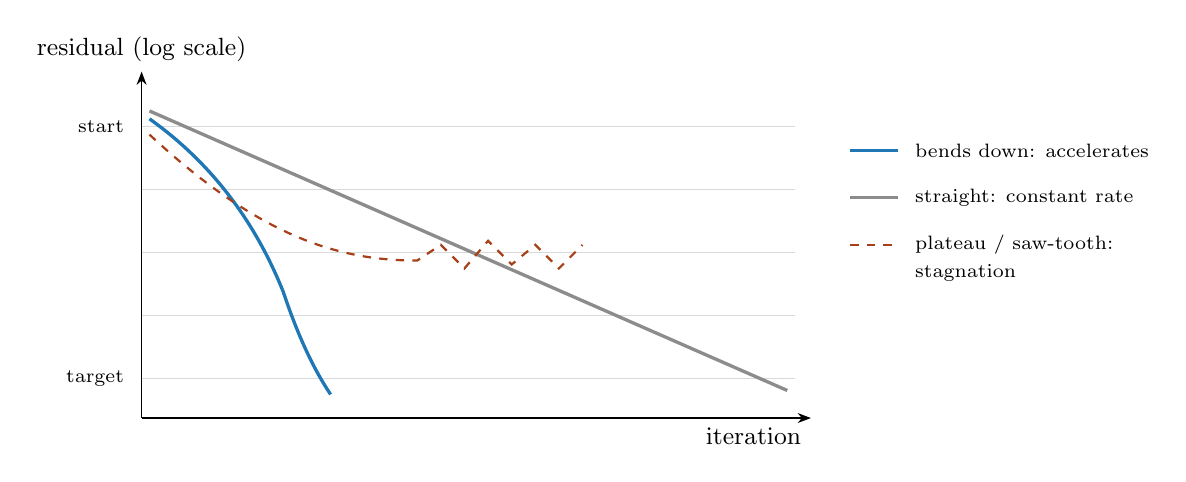
\begin{tikzpicture}[>=Stealth, font=\small]
  \draw[->] (0,0) -- (8.5,0) node[below left] {iteration};
  \draw[->] (0,0) -- (0,4.4) node[above] {residual (log scale)};
  \foreach \y in {0.5,1.3,2.1,2.9,3.7} \draw[gray!30] (0,\y) -- (8.3,\y);
  \node[anchor=east, font=\scriptsize, align=right] at (-0.1,3.7) {start};
  \node[anchor=east, font=\scriptsize, align=right] at (-0.1,0.5) {target};
  % coupled-like curve
  \draw[very thick, cfcoupled] (0.1,3.8) .. controls (0.8,3.3) and (1.4,2.6) .. (1.8,1.6)
     .. controls (2.0,1.0) and (2.2,0.6) .. (2.4,0.3);
  % straight line
  \draw[very thick, cfnative] (0.1,3.9) -- (8.2,0.35);
  % stagnating
  \draw[thick, cfpit, dashed] (0.1,3.6) .. controls (1.5,2.3) and (2.5,2.0) .. (3.5,2.0)
     -- (3.8,2.2) -- (4.1,1.9) -- (4.4,2.25) -- (4.7,1.95) -- (5.0,2.2) -- (5.3,1.9) -- (5.6,2.2);
  % legend
  \begin{scope}[shift={(9.0,3.4)}, font=\scriptsize]
    \draw[very thick, cfcoupled] (0,0) -- (0.6,0);
    \node[anchor=west] at (0.7,0) {bends down: accelerates};
    \draw[very thick, cfnative] (0,-0.6) -- (0.6,-0.6);
    \node[anchor=west] at (0.7,-0.6) {straight: constant rate};
    \draw[thick, cfpit, dashed] (0,-1.2) -- (0.6,-1.2);
    \node[anchor=west] at (0.7,-1.2) {plateau / saw-tooth:};
    \node[anchor=west] at (0.7,-1.55) {stagnation};
  \end{scope}
\end{tikzpicture}
\caption{Illustrative sketch (not data) of three typical residual histories
on a logarithmic axis.}
\label{fig:readconv}
\end{figure}

\paragraph{What are $C_d$ and $C_l$?}
The force the air exerts on a body is split into \emph{drag} $F_D$ (along
the free-stream direction) and \emph{lift} $F_L$ (perpendicular to it; for a
race car the interesting part is negative lift, i.e.\ downforce). They are
made dimensionless with the dynamic pressure of the free stream and a
reference area $A$:
\begin{equation*}
  C_d = \frac{F_D}{\tfrac12\rho U_\infty^2 A},\qquad
  C_l = \frac{F_L}{\tfrac12\rho U_\infty^2 A}.
\end{equation*}
In OpenFOAM they are computed by the \code{forceCoeffs} function object.
In a steady RANS run they settle to constant values as the solver
converges; the benchmark uses exactly this settling as its convergence
criterion (Section~\ref{sec:protocol}).

\paragraph{Relative $L_2$ difference.} To compare two profiles (say, the
velocity along a line from coupledFoam and from \code{simpleFoam}), one
takes the root of the sum of squared differences at all points, divided by
the root of the sum of squared reference values. A value of $10^{-3}$ means
the curves differ by about a tenth of a per cent of their typical size; a
value of $10^{-6}$ means they are identical for all practical purposes.

\paragraph{What does ``pass'' mean?} Every test has pass criteria fixed
in the specification before any result was known, and they may only be
tightened, never relaxed. The main criterion is always a comparison with
\code{simpleFoam} on the \emph{identical} mesh, schemes and boundary
conditions: both solvers solve the same discrete equations, so their
converged answers should agree closely. Agreement with experiments is
reported where available but is a property of the turbulence model and the
mesh, not of the solver.

\subsection{Test protocol}\label{sec:testprotocol}

Unless stated otherwise, every case is run on 1 and on 4 parallel ranks, and
both must pass, with integral quantities agreeing between rank counts to
$10^{-4}$ relative. Development runs trap floating-point exceptions (a
division by zero or an invalid operation aborts the run); any trap is a
failure. Below the case tests sit unit tests of the individual components
(block inversion, block matrix product against OpenFOAM's own, double
reductions, the multigrid on a model problem, FGMRES with a deliberately
changing preconditioner). Table~\ref{tab:tests} lists all test records
produced so far.

\cftable{tests}{Test results.}{tab:tests}

\paragraph{How to read Table~\ref{tab:tests}.} One row per test record
(\code{\_np1}, \code{\_np4}: run on 1 or 4 ranks). ``pass'' is the verdict
of the test's own criteria; ``iterations'' and ``final R'' refer to the
outer iteration of coupledFoam; ``wall'' is the elapsed time of the run on
a \emph{shared} development machine and is not a benchmark result;
``key metric'' shows the most important measured quantity of the test,
e.g.\ \code{l2rel\_u} (relative $L_2$ difference of the $u$ profile against
\code{simpleFoam}) or \code{crossRankRelDiff} (difference between the 1- and
4-rank solutions).

\subsection{T0: lid-driven cavity}\label{sec:t0}

\paragraph{What it is.} A square box filled with fluid whose top wall (the
lid) slides sideways; the fluid is dragged along and forms a large rotating
vortex, with small counter-rotating vortices in the corners. Laminar, 2D,
$128\times128$ cells, at Reynolds numbers 100 and 1000, with the
\code{linearUpwind} scheme. It is the classical first test of any
incompressible solver; reference data by Ghia et al.~\cite{Ghia1982}.

\paragraph{What it tests.} The core of the solver: the block assembly,
Rhie--Chow, the closed-domain pressure reference, the precision design, and
whether a float linear solver can reach a residual of $10^{-8}$.
Pass: $R<10^{-8}$ within 300 iterations, centreline profiles within
$10^{-3}$ relative $L_2$ of \code{simpleFoam}, no floating-point trap, no
clamped coefficients.

\paragraph{Result at $Re=100$.} coupledFoam converged to $R<10^{-8}$ in
\cfnum{TZeroReOneZeroZeroIterations} outer iterations; \code{simpleFoam}
needed \cfnum{TZeroReOneZeroZeroNativeIterations} iterations to its own
tolerance of $10^{-8}$. The centreline profiles agree to a relative $L_2$
difference of \cfsci{TZeroReOneZeroZeroLTwou} in $u$ and
\cfsci{TZeroReOneZeroZeroLTwov} in $v$, far below the threshold of
$10^{-3}$. Two solvers that solve the same discrete equations have arrived
at the same answer.

\cffigure{T0_Re100_profiles}{T0, lid-driven cavity at $Re=100$: centreline
profiles $u(y)$ and $v(x)$, coupledFoam against simpleFoam.}{fig:t0profiles}

\paragraph{How to read Figure~\ref{fig:t0profiles}.} Left: the horizontal
velocity $u$ (divided by the lid speed) along the vertical line through the
centre of the box, plotted against height. Near the top it approaches the
lid speed; lower down it is negative, which is the return flow of the
vortex. Right: the vertical velocity $v$ along the horizontal centreline.
\code{simpleFoam} is drawn as a thick line, coupledFoam as a thin dashed
line on top of it. \emph{Good} means: the two lines are indistinguishable.

\cffigure{T0_Re100_np1_history}{T0, $Re=100$, one rank: combined residual $R$
of coupledFoam and native initial residuals of simpleFoam (left); CFL number
and line-search factor $\omega$ (right).}{fig:t0history}

\paragraph{How to read Figure~\ref{fig:t0history}.} Left: residuals against
iteration on a log axis; coupledFoam's $R$ together with the $p$ and $U_x$
initial residuals of \code{simpleFoam}. The \emph{shapes} matter: the
coupled residual falls steeply within few iterations, the native ones
decrease slowly over far more iterations. Right: the CFL number (log axis) ramps up from its start
value to the maximum, and the line-search factor $\omega$ (right axis,
between 0 and 1) shows whether full steps were taken. A smooth CFL ramp and
$\omega$ at one are the picture of an untroubled run.

\cffigure{T0_Re1000_profiles}{T0, lid-driven cavity at $Re=1000$: centreline
profiles, coupledFoam against simpleFoam.}{fig:t0profilesRe1000}

\cffigure{T0_Re1000_np1_history}{T0, $Re=1000$, one rank: residuals (left);
CFL number and line-search factor $\omega$ (right).}{fig:t0historyRe1000}

\paragraph{$Re=1000$} is the harder variant: the vortex is stronger, the
corner vortices are larger and the convection scheme matters more. This is
the case of the smoother story (Section~\ref{sec:smoothers}).
Figures~\ref{fig:t0profilesRe1000} and~\ref{fig:t0historyRe1000} are read in
the same way as those for $Re=100$; the measured values are listed in
Table~\ref{tab:tests}.

\subsection{T1--T5: from 2D turbulence to 3D vehicles}\label{sec:t1t5}

\begin{description}
\item[T1, pitzDaily (SST).] The OpenFOAM tutorial of a 2D channel with a
  backward-facing step and a contraction, about 12\,k cells, turbulent. It
  tests turbulence coupling and inlet/outlet boundary conditions. Pass:
  $R<10^{-6}$ within 400 iterations; pressure drop from inlet to outlet
  within 1\,\% of \code{simpleFoam}; the CFL number at least 100 without
  cuts after iteration 100; no rollbacks. \emph{Why this matters:} the
  pressure drop is the simplest integral engineering quantity, and the CFL
  criterion checks that the solver runs at full speed once past the
  start-up.
\item[T2, backward-facing step (SST).] A 2D channel whose floor steps down;
  the flow separates at the step and reattaches further downstream.
  Experimental reference: Driver and Seegmiller~\cite{Driver1985}. Pass: the
  reattachment length (where the wall shear stress on the lower wall changes
  sign) within 2\,\% of \code{simpleFoam}, and at least two times fewer
  outer iterations to a residual of $10^{-5}$ (the iteration definition for
  the two solvers is fixed in D-024). \emph{Why this matters:}
  separation and reattachment are the phenomena that dominate the wake and
  diffuser of a car.
\item[T3, airFoil2D (SST and GEKO).] The 2D airfoil tutorial. Pass: $C_l$
  and $C_d$ within 0.5\,\% of \code{simpleFoam}, for each turbulence model,
  with identical settings; empty dynamic remediation set at convergence.
  \emph{Why this matters:} lift and drag of a wing profile, which is
  what front and rear wings are.
\item[T4, motorBike.] The OpenFOAM motorbike-with-rider tutorial meshed with
  \code{snappyHexMesh}: a coarse mesh of about 350\,k cells (T4a) and a
  finer mesh (T4b, retargeted to 1--2\,M cells, D-031), run in parallel.
  Pass: the averaged $C_d$ and $C_l$ have settled and agree with
  \code{simpleFoam} (2\,\% for $C_d$; averaged criterion for the oscillating
  wake, D-042); static remediation set at most 1\,\% of the cells; no
  rollbacks. \emph{Why this matters:} this is the first case with a
  complex 3D geometry and an automatically generated mesh with real
  bad cells, the closest test to a car.
\item[T5, Ahmed body, $25^\circ$ slant.] A simplified car body with a slanted
  rear, the standard automotive bluff-body benchmark~\cite{Ahmed1984}; half
  model, 5--8\,M cells, $U_\infty=\SI{40}{m/s}$, SST with wall functions.
  Pass: as T4 (averaged criterion, D-042); the comparison with the
  experimental $C_d=0.285$ ($\pm10$\,\%) is for information only.
  \emph{Why this matters:} it is the size class and flow type of a
  vehicle simulation: separation on the slant, a wake, ground effect.
  \emph{Status:} deferred. The project owner decided not to run T5 in the
  present test campaign (D-063); the case is kept for a later campaign,
  and this document contains no T5 results.
\end{description}

Three further tests check specific features:
\begin{description}
\item[T-restart.] T1 and T3 are split at iteration 150 and restarted: the
  iteration count must match the continuous run within two iterations, the
  final quantities within $10^{-5}$, and the recomputed fluxes must match
  the stored ones.
\item[T-fpe.] A deliberately brutal start of T1: zero initial velocity, no
  potential-flow initialisation, start CFL 200, no upwind start-up. The
  solver must not crash; rollbacks are allowed; it must recover and
  converge. \emph{Why this matters:} this is the test of the safety net
  (line search, remediation, sentinel).
\item[T-mrf.] The \code{mixerVessel2D} tutorial with a rotating MRF zone;
  torque compared with \code{simpleFoam}. Informational only, because the
  specification gave no threshold (D-009).
\end{description}

\cftable{validation}{Validation, T1--T4: integral quantities (pressure drop,
reattachment length, $C_l$, $C_d$, torque) of coupledFoam and simpleFoam and
their relative differences.}{tab:validation}

\paragraph{How to read Table~\ref{tab:validation}.} One row per case and
quantity: the value from coupledFoam, the value from \code{simpleFoam} on the
same mesh, their relative difference, the tolerance of the test, and the
verdict. \emph{Good} means: the relative difference is well below the
tolerance. A difference close to the tolerance on a case with many
remediated cells would point to the local upwinding of
Section~\ref{sec:remediation}. The wake behind the motorbike (rows marked
\textsuperscript{\dag}) never settles, not even in
\code{simpleFoam}, so for T4 the table compares averages over a window of
the last iterations of each run, the same window length for both solvers
(400 iterations on the motorbike, D-068), shown as mean $\pm$ standard
deviation. There, ``converged'' means that the averages of the two halves
of that window differ by at most 1\,\% or by 0.005, whichever is larger
(D-042 and its addenda). Their tolerances are
correspondingly coarser (2\,\% for $C_d$, and an absolute 0.01 for the small
$C_l$), a change the project owner approved for exactly these cases.
Two numbers can agree by luck, so the averaged flow fields of the two
solvers are also subtracted cell by cell. The column ``field RMS dU / dp''
gives the typical size of that difference, relative to the free-stream
speed and to the free-stream dynamic pressure. The proposed pass limit is
2\,\%.

\paragraph{Watching the forces settle.} Figures~\ref{fig:ovWing}
and~\ref{fig:ovMotorbike} show how the drag ($C_d$, left) and lift ($C_l$,
right) develop while each solver runs, for the wing and the motorbike.
Orange is \code{simpleFoam}, blue is coupledFoam, and the
horizontal axis is the time on the clock, so the two solvers are compared
fairly: a curve that settles further left belongs to the faster solver.
The thin line, or for long runs a light band spanning the minimum and
maximum of each group of iterations, is the value after every iteration;
where one run is much shorter, a second row zooms on its time range. The
dashed line is
its running average over the averaging window, and the dotted horizontal
line the final average that enters Table~\ref{tab:validation}. Two
dotted lines at the same height mean the solvers agree. Every quantity of
every run, iteration by iteration, is in the appendix
(Section~\ref{app:histories}).

\cffigure{loads_overview_wing}{Wing (T3 airfoil, SST and GEKO): drag and
lift over wall-clock time, simpleFoam (orange) and coupledFoam
(blue).}{fig:ovWing}
\cffigure{loads_overview_motorbike}{Motorbike (T4a coarse, T4b fine): drag
and lift over wall-clock time.}{fig:ovMotorbike}

\cffigure{remediation_history}{Size of the dynamic remediation set over the
iterations, one panel per run.}{fig:remediation}

\cftable{remediation_categories}{Remediation cells per category and test
run.}{tab:remcat}

\paragraph{How to read Table~\ref{tab:remcat}.} One row per test run: the
number of pre-selected cells in each category (where the run records
them), their total and share of the mesh, and the largest and the final
size of the dynamic set. A static share above about 1\,\% points to a mesh
that needs attention; a dynamic set that is not empty at the end means
some cells were still misbehaving when the run stopped.

\paragraph{How to read Figure~\ref{fig:remediation}.} The number of cells in
the dynamic remediation set against the iteration. Typical and healthy: a
peak during the early, violent iterations, then decay to (nearly) zero as
the flow settles. A set that stays large, or grows late in the run, points
at a persistent local problem (mesh or boundary condition).

\clearpage
\subsection{Looking at the flow: pictures of the two solutions}\label{sec:flowpics}

Numbers such as a drag coefficient can agree by luck, when two errors
cancel. The honest check is to look at the whole flow. This section shows
the solutions of both solvers side by side and, as a third picture, their
difference. Everything is computed from the result files of the runs by
\code{bench/plot\_fields2d.py} (2D cases) and \code{bench/render\_fields.py}
(3D cases, rendered with ParaView).\pro{Flow fields}

\paragraph{How to read the field pictures.} Each figure has three panels.
The first two show the same quantity for coupledFoam and for
\code{simpleFoam}, with the \emph{same} colour scale, so equal colours mean
equal values. The white lines in the velocity pictures are streamlines:
lines that follow the flow direction, so vortices appear as closed loops.
The third panel is the difference coupledFoam minus \code{simpleFoam}; its
colour scale is centred on zero: white means ``no difference'', red means
coupledFoam is higher, blue means it is lower. The numbers on its
colour bar matter: the scale is chosen from the data, so even tiny differences
look colourful. The title gives the RMS (a typical size) and the maximum of
the difference. All values are made dimensionless: the velocity divided by
a reference speed $U_{ref}$ (the lid speed, the inlet speed or the
free-stream speed), the pressure as the pressure coefficient
$C_p=(p-p_0)/(\tfrac12U_{ref}^2)$, where $C_p=1$ is the pressure at a
stagnation point and negative values are suction. \emph{Good} means: the
first two panels look identical and the difference is small compared with
one.

\paragraph{T0, the cavity.} The big vortex fills the box; the difference
between the solvers is about \cfnum{FldTZeroReOneZeroZeroURms} of the lid
speed on average, i.e.\ invisible. The only coloured spots in the difference
panel are the two upper corners, where the sliding lid meets the fixed
walls. There the flow is forced to jump from lid speed to zero, the pressure
becomes very large, and every solver is least accurate.

\cffigure{fields_T0_Re100_U}{T0, $Re=100$: speed with streamlines,
coupledFoam (left), simpleFoam (middle), difference (right).}{fig:fldTzeroU}
\cffigure{fields_T0_Re100_p}{T0, $Re=100$: pressure coefficient and
difference.}{fig:fldTzeroP}
\cffigure{fields_T0_Re1000_U}{T0, $Re=1000$: speed with streamlines and
difference.}{fig:fldTzerothousandU}
\cffigure{fields_T0_Re1000_p}{T0, $Re=1000$: pressure coefficient and
difference.}{fig:fldTzerothousandP}

\clearpage
\paragraph{T1, pitzDaily.} Long, flat pictures, so the three panels are
stacked: coupledFoam on top, \code{simpleFoam} in the middle, the difference
at the bottom. The dark region behind the step is the recirculation zone,
where the flow turns around (closed streamlines). The difference is about
\cfnum{FldTOneURms} of the inlet speed on average.

\paragraph{How to read the profile pictures.} Figure~\ref{fig:prTone} cuts
the channel at several positions behind the step (labelled by their
distance in step heights, $x/h$). At each position the horizontal velocity
is drawn as a curve starting from the thin vertical line: the further the
curve bulges to the right, the faster the flow at that height; a bulge to
the left of the line is backflow. Thick orange is \code{simpleFoam}, dashed
blue is coupledFoam. \emph{Good} means: only one curve is visible.

\cffigure{fields_T1_U}{T1 pitzDaily: speed with streamlines, coupledFoam
(top), simpleFoam (middle), difference (bottom).}{fig:fldToneU}
\cffigure{fields_T1_p}{T1 pitzDaily: pressure coefficient and
difference.}{fig:fldToneP}
\cffigure{profiles_T1}{T1 pitzDaily: velocity profiles behind the
step.}{fig:prTone}

\clearpage
\paragraph{T2, backward-facing step.} The flow detaches at the corner of
the step, forms a long, flat recirculation bubble and reattaches further
downstream. The largest difference between the solvers is in the thin
shear layer that leaves the step corner, where the velocity changes very
quickly over a short distance. The lower picture of
Figure~\ref{fig:prTtwo} shows the skin friction $C_f$ on the floor: positive
where the flow near the floor moves downstream, negative inside the bubble.
Where it crosses zero after the step, the flow reattaches: that point is
the ``reattachment length'' of the test. Both curves cross at the same
place. (The narrow orange spike near $x/h\approx1.4$ exists only in the
\code{simpleFoam} run, which never reached its residual target.)

\cffigure{fields_T2_U}{T2 backward-facing step: speed with streamlines,
coupledFoam (top), simpleFoam (middle), difference (bottom).}{fig:fldTtwoU}
\cffigure{fields_T2_p}{T2 backward-facing step: pressure coefficient and
difference.}{fig:fldTtwoP}
\cffigure{profiles_T2}{T2: velocity profiles (top) and skin friction on the
floor (bottom).}{fig:prTtwo}

\clearpage
\paragraph{T3, the airfoil: where the pictures show a problem.} Here the
pictures are more useful than the table. With the GEKO turbulence model the
flow around the airfoil looks the same in both solvers, but the surface
pressure (Figure~\ref{fig:prTthreegeko}) differs near the front of the upper
side: coupledFoam produces a higher suction peak. The upper curve is the
suction side (it carries the lift), so a difference there means a
difference in lift, and this is the lift difference that fails the test in
Table~\ref{tab:validation}. With the SST model the coupledFoam run did not
converge: above the airfoil it shows a region of large vortices that the
\code{simpleFoam} solution does not have, and the difference panel is
coloured almost everywhere. These pictures show the current state of the
test records, not a solved problem.

\paragraph{How to read the airfoil pressure plot.} The horizontal axis runs
along the chord from the nose ($x/c=0$) to the tail ($x/c=1$). The vertical
axis is $-C_p$, drawn upside down on purpose, so that suction points up.
The upper curve is the upper (suction) side, the lower curve the lower
(pressure) side; the area between them is proportional to the lift.

\cffigure{fields_T3_GEKO_U}{T3 airfoil, GEKO: speed with streamlines around
the airfoil, coupledFoam (top), simpleFoam (middle), difference
(bottom).}{fig:fldTthreegekoU}
\cffigure{fields_T3_GEKO_p}{T3 airfoil, GEKO: pressure coefficient and
difference.}{fig:fldTthreegekoP}
\cffigure{profiles_T3_GEKO}{T3 airfoil, GEKO: surface pressure along the
chord.}{fig:prTthreegeko}
\cffigure{fields_T3_kOmegaSST_U}{T3 airfoil, SST: speed with streamlines;
the coupledFoam run did not converge.}{fig:fldTthreesstU}
\cffigure{profiles_T3_kOmegaSST}{T3 airfoil, SST: surface pressure along
the chord.}{fig:prTthreesst}

\clearpage
\paragraph{T4: 3D pictures.} For the motorbike the pictures are rendered
with ParaView. The first picture shows the body with the surface mesh drawn
on it: every small polygon is the face of one cell touching the body, which
shows where the mesh generator placed fine and coarse cells. The slice
pictures cut the flow with two flat planes, a vertical one through the
middle of the body (side view) and a horizontal one at 20\,\% of the body
height (top view); the body itself is drawn in grey. The left column is
\code{simpleFoam}, the right column coupledFoam; a grey panel saying
``results pending'' means that run has not finished yet, and the picture
fills in automatically when the report is regenerated. The colour ranges
are fixed (speed from 0 to 1.3 times the free-stream speed, $C_p$ from
$-1.5$ to 1), so pictures of different runs can be compared directly. The
dark band behind the body is the wake, the slow region the body leaves
behind. (The Ahmed body T5 is not run in the present campaign, by decision
of the project owner, D-063.)

\paragraph{How to read the difference pictures.} Two pictures of the same
wake look alike to the eye even when the velocities differ by several per
cent, so the decisive comparison subtracts one solution from the other. The
wake of the motorbike keeps moving from iteration to iteration, even in
\code{simpleFoam}; both solvers therefore average their fields over the
same long window of iterations (the window of the force averages), and the
utility \code{coupledFieldCompare} subtracts the averaged fields cell by
cell: coupledFoam minus \code{simpleFoam}. Two quantities are shown, both
without units: the difference of the streamwise velocity divided by the
free-stream speed, $\Delta u_x/U_\infty$, and the difference of the pressure
coefficient, $\Delta C_p$ (pressure difference divided by the free-stream
dynamic pressure $\tfrac12U_\infty^2$). The colour scale is centred on zero
and the same in every picture: white means ``no difference'', red means
coupledFoam is higher, blue means it is lower, and the darkest colours mean
a difference of 20\,\% of $U_\infty$ (or of the dynamic pressure) or more.
Typical patterns: a red band next to a blue band behind the body means the
wake of one solver is slightly shifted or shorter; a red--blue pair on the
body surface marks a place where the flow separates at a slightly different
position, which changes the drag. \emph{Good} means: mostly white, with
coloured regions confined to the thin shear layers of the wake, where the
averages of two oscillating solutions converge slowest. The typical size of
these differences over the whole domain is the ``field RMS'' column of
Table~\ref{tab:validation}.\pro{Flow fields}

\cffigure{render_T4a_geometry}{T4a motorbike (coarse mesh): body surface
mesh.}{fig:rTfouraGeo}
\cffigure{render_T4a_slice_U}{T4a: speed on the vertical mid-plane (top)
and the horizontal plane (bottom), simpleFoam (left) and coupledFoam
(right).\cfrenderflag{TFoura}}{fig:rTfouraU}
\cffigure{render_T4a_surface_Cp}{T4a: pressure coefficient on the
body.\cfrenderflag{TFoura}}{fig:rTfouraCp}
\cffigure{render_T4a_delta_slices}{T4a: difference of the averaged fields,
coupledFoam minus simpleFoam: streamwise velocity (top) and pressure
coefficient (bottom) on the vertical plane (left) and the horizontal plane
(right). White: no difference; red: coupledFoam higher; blue: coupledFoam
lower.\cfrenderflag{TFoura}}{fig:rTfouraDelta}
\cffigure{render_T4a_delta_surface}{T4a: difference of the averaged surface
pressure coefficient on the body, coupledFoam minus
simpleFoam.\cfrenderflag{TFoura}}{fig:rTfouraDeltaS}
\clearpage
\IfFileExists{figures/render_T4b_delta_slices.png}{%
\cffigure{render_T4b_geometry}{T4b motorbike (fine mesh): body surface
mesh.}{fig:rTfourbGeo}
\cffigure{render_T4b_slice_U}{T4b: speed on the vertical mid-plane (top)
and the horizontal plane (bottom), simpleFoam (left) and coupledFoam
(right).\cfrenderflag{TFourb}}{fig:rTfourbU}
\cffigure{render_T4b_slice_p}{T4b: pressure coefficient on the two
planes.\cfrenderflag{TFourb}}{fig:rTfourbP}
\cffigure{render_T4b_surface_Cp}{T4b: pressure coefficient on the body:
red is high pressure (the flow runs into the surface), blue is
suction.\cfrenderflag{TFourb}}{fig:rTfourbCp}
\cffigure{render_T4b_delta_slices}{T4b: difference of the averaged fields,
coupledFoam minus simpleFoam, on both planes.\cfrenderflag{TFourb}}{fig:rTfourbDelta}
\cffigure{render_T4b_delta_surface}{T4b: difference of the averaged surface
pressure coefficient on the body.\cfrenderflag{TFourb}}{fig:rTfourbDeltaS}
\clearpage}{%
\paragraph{T4b.} The fine motorbike mesh is run only after the coarse one
has been accepted (D-063); its pictures are added when the report is
regenerated after that run.}
\clearpage

% =============================================================================
\section{Performance: is it faster?}\label{sec:perf}
% =============================================================================

\subsection{The benchmark protocol in plain words}\label{sec:protocol}

\paragraph{Contestants.} For each case (T1, T2, T3 with SST and with GEKO,
T4a, T4b), with identical mesh, decomposition, schemes, turbulence model
and boundary conditions:
\begin{description}
\item[A] \code{simpleFoam} with the tutorial's own settings (for pitzDaily
  and the backward-facing step the tutorial already uses SIMPLEC, D-025);
\item[B] \code{simpleFoam} SIMPLEC with relaxation factors 1.0 for $p$ and
  0.9 for $\Uv$, $k$, $\omega$: the tuned native baseline;
\item[C] coupledFoam with default settings (since D-043: V-cycle multigrid
  with a damped ILU(0) smoother);
\item[D] coupledFoam with the simple block-diagonal preconditioner instead
  of multigrid (shows what the multigrid is worth);
\item[H] coupledFoam with the K-cycle instead of the V-cycle on T1--T3 and
  the coarse motorbike (shows what the cycle choice is worth); H-tune adds
  the automatic cycle controller on T1 and T2. A configuration E with a
  fixed V-cycle was planned as well; since D-043 it is identical to C and
  is no longer run (D-068). The ``E-'' variants change one setting of C
  each.
\end{description}
Not every case gets every contestant in the present campaign (D-063): most
runs are on the light cases T1--T3, the coarse motorbike T4a gets the full
set, the fine T4b only a few runs after T4a has been accepted, and the Ahmed
body T5 is not run at all (deferred by the project owner).
In addition, T1 and T3-SST are run with a fixed linear tolerance instead of
Eisenstat--Walker (labelled F in the figures) and with Anderson acceleration
(G).

\paragraph{Finish line.} Each solver's own stopping rule is switched off and
a fixed number of iterations is run. Afterwards the harness finds, for all
solvers in the same way, the first iteration at which the force
coefficients have settled: over the last 100 iterations, $C_d$ and $C_l$
vary by at most 0.2\,\% of their mean (for T1 and T2, the pressure drop).
This is the ``convergence iteration''. For the motorbike (T4), whose
forces never settle, it is instead the first iteration at which their
average over a window of 400 iterations drifts by at most 1\,\% or 0.005,
whichever is larger (D-042 and its addenda). The window is the same for
both solvers (D-068). An earlier version took half of each run's own
length as the window; since \code{simpleFoam} was given far more
iterations than coupledFoam, its window was longer, and it could not be
declared converged before the end of that longer window. That version
made the native solver look slower than it is, and it is reported only as
a sensitivity value.

\paragraph{Stopwatch.} Every rank runs under \code{/usr/bin/time}, which
records the wall-clock time and the CPU time. The totals of the whole run
are scaled to the convergence iteration using the solver's own time log
(D-025). CPU time is summed over ranks and reported in CPU-hours. Peak
memory is the maximum resident memory of each rank. Where a run starts
from a \code{potentialFoam} solution (every coupledFoam run, and the
tutorial configuration A of \code{simpleFoam} on the motorbike), that
preparation is counted too. On T1--T3 each configuration is run three
times and the median is reported; on the motorbike each is run once
(12-hour budget, D-059).

\paragraph{Machine.} 16 physical cores, 94\,GB of memory visible to WSL; MPI
ranks bound to physical cores; the motorbike runs use 10 ranks (D-031), the
scaling test up to 16 (D-059); benchmarks run when no other solver is
running, and the machine load before each run is recorded (D-007).

\begin{whyitmatters}{why this protocol is fair}
  Both solvers are stopped by the same, physically meaningful criterion
  (the forces do not change any more), not by their incomparable residuals;
  both get the same hardware and the same mesh; and the native solver gets
  its best of two settings. A speed-up measured this way is the time
  actually saved in practice.
\end{whyitmatters}

\subsection{How to read speed-ups}

The speed-up is
\begin{equation*}
  \text{speed-up}=\frac{\text{time of the better native configuration (A or B)}}
                      {\text{time of coupledFoam (C)}} ,
\end{equation*}
computed once with wall-clock time and once with CPU-hours. A value above
one means coupledFoam is faster; 2.0 means it needs half the time; a value
below one means it is slower. The two can differ: if one solver scales
worse in parallel, it may still finish sooner in wall time but consume
more CPU-hours, or vice versa.

\begin{table}[tbp]
\centering\small
\caption{Speed-up of coupledFoam against the better native configuration,
from the benchmark (values $>1$: coupledFoam faster). Generated numbers;
``pending'' where the benchmark has not been run yet.}
\label{tab:speedups}
\begin{tabular}{lcc}
\toprule
case & speed-up (wall-clock) & speed-up (CPU-hours)\\
\midrule
T1 pitzDaily & \cfnum{SpeedupWallTOne} & \cfnum{SpeedupCpuTOne}\\
T2 backward-facing step & \cfnum{SpeedupWallTTwo} & \cfnum{SpeedupCpuTTwo}\\
T3 airfoil, SST & \cfnum{SpeedupWallTThreeSST} & \cfnum{SpeedupCpuTThreeSST}\\
T3 airfoil, GEKO & \cfnum{SpeedupWallTThreeGEKO} & \cfnum{SpeedupCpuTThreeGEKO}\\
T4a motorBike, coarse & \cfnum{SpeedupWallTFoura} & \cfnum{SpeedupCpuTFoura}\\
T4b motorBike, fine & \cfnum{SpeedupWallTFourb} & \cfnum{SpeedupCpuTFourb}\\
T5 Ahmed body & \multicolumn{2}{c}{deferred (D-063)}\\
\bottomrule
\end{tabular}
\end{table}

Table~\ref{tab:speedups} extracts the speed-ups; the full executive summary
with absolute times and the memory ratio is Table~\ref{tab:summary}.

\paragraph{Convergence point chosen by the user.} An automatic criterion is
only a rule of thumb. For the wing and the motorbike the user
may inspect the load histories in the appendix and name an earlier iteration
$N$ from which the run is considered converged (\texttt{report/user\_%
convergence.json}, D-060). Wall time and CPU-hours are then counted up to $N$,
and $C_d$ and $C_l$ are averaged from $N$ to the end of the run. The stop
criteria of the runs themselves are unchanged, so a user iteration can only
move the convergence point earlier. Table~\ref{tab:convchoice} shows the
automatic point next to the user's; in the load histories the automatic point
is dash-dotted and the user's point solid.

\cftable{convergence_choice}{Convergence point of the force cases: automatic
and user choice (D-060).}{tab:convchoice}

\cftable{executive_summary}{Executive summary: time to convergence (identical
window criterion), best native configuration against coupledFoam, as
wall-clock time and CPU-hours.}{tab:summary}

\paragraph{How to read Table~\ref{tab:summary}.} Per case: the wall time and
CPU-hours of the best native configuration and of coupledFoam, the two
speed-ups, and the memory ratio (coupledFoam's peak memory divided by the
native one; a value above one means coupledFoam needs more memory, which is
expected because of the $4\times4$ blocks).

\subsection{The benchmark figures}

\cffigure{bench_wall}{Wall-clock time to convergence (median of the
repeats: three on T1--T3, one on the motorbike) per case and
configuration.}{fig:benchwall}

\cffigure{bench_cpu}{CPU time to convergence (CPU-hours summed over ranks,
median of the repeats).}{fig:benchcpu}

\paragraph{How to read Figures~\ref{fig:benchwall} and~\ref{fig:benchcpu}.}
One group of bars per case, one bar per configuration (legend). The
vertical axis is \emph{logarithmic}: equal distances mean equal
\emph{factors}, so a bar one grid step lower is ten times faster. Compare
the coupledFoam bar (C) with the lower of the two \code{simpleFoam} bars
(A, B). Bar D shows the cost of dropping the multigrid, H the effect of
the K-cycle instead of the default V-cycle.

\cffigure{bench_iters}{Outer iterations to convergence. Shown for
completeness; the decisive metrics are those of Figures~\ref{fig:benchwall}
and~\ref{fig:benchcpu}.}{fig:benchiters}

\paragraph{Figure~\ref{fig:benchiters}} shows iteration counts. coupledFoam
is expected to need far fewer; that alone proves nothing
(Section~\ref{sec:fair}). The ratio of the iteration ratio to the time
ratio gives how much more expensive a coupled iteration is.

\cffigure{bench_breakdown}{coupledFoam time per outer iteration split into
assembly, linear solve and turbulence.}{fig:breakdown}

\paragraph{How to read Figure~\ref{fig:breakdown}.} For each case, one bar
of coupledFoam's average time per outer iteration, split into building the
system (assembly), solving it (linear solve) and the turbulence update. In
a coupled solver the linear solve normally dominates; if assembly or
turbulence were dominant, optimising the multigrid would not help much.

\cffigure{bench_memory}{Peak memory, sum of the per-rank maximum RSS.}{fig:memory}

\paragraph{Memory (Figure~\ref{fig:memory}).} The sum over all ranks of
each rank's peak memory. coupledFoam stores $4\times4$ blocks and the
multigrid hierarchy, so it needs more memory than \code{simpleFoam}; the
float storage (Section~\ref{sec:precision}) halves the matrix part of that
overhead. For planning a large case, the ratio between the bars is the
number to scale with.

\cffigure{scaling}{Strong scaling on T4a (1 to 16 ranks): time per iteration and parallel
efficiency of coupledFoam and simpleFoam. Pass: the parallel efficiency of
coupledFoam at the largest rank count is at least 80\,\% of that of
simpleFoam.}{fig:scaling}

\paragraph{Scaling (Figure~\ref{fig:scaling}).} \emph{Strong scaling}
means: the same mesh, more ranks. Left: time per iteration against the
number of ranks, both on log axes; ideal scaling is a straight line
falling with slope $-1$ (twice the ranks, half the time). Right:
\emph{parallel efficiency}
\begin{equation*}
  E(n)=\frac{t(n_0)\,n_0}{t(n)\,n},
\end{equation*}
with $t(n)$ the time per iteration on $n$ ranks and $n_0$ the smallest
rank count; $E=1$ is perfect, $E=0.5$ means half of the added cores are
wasted on communication and waiting. The scaling test runs on the coarse
motorbike T4a with 1, 2, 4, 8, 12 and 16 ranks on physical cores (D-059;
the specification planned the finer T4b), with the pass threshold
unchanged. Multigrid solvers typically lose
some efficiency on coarse levels; processor agglomeration
(Section~\ref{sec:procagg}) is the countermeasure.

\cftable{gamg_levels}{Block-GAMG hierarchy per case: levels, cells and ranks
per level, coarsening ratios, operator complexity, coarsest-level
solver.}{tab:gamglevels}

\paragraph{How to read Table~\ref{tab:gamglevels}.} For each run: how many
multigrid levels were built, the \code{mergeLevels} value finally used
(larger than 2 means the coarsening rule forced more aggressive
coarsening), the operator complexity $C_{\mathrm{op}}$ (total size of all
level matrices relative to the finest; must be at most 1.5), and the number
of cells on each level. Dividing consecutive cell counts gives the
coarsening ratios of Section~\ref{sec:amg}.

\cffigure{cycle_comparison}{Unit test (not a benchmark): Krylov iterations
and solve time of the V-, F-, W- and K-cycles on the block-Poisson system
of the cavity mesh.}{fig:cycles}

\paragraph{Cycles (Figure~\ref{fig:cycles}).} Krylov iterations (left) and
solve time (right) per cycle type. A stronger cycle needs fewer Krylov
iterations but each is more expensive; the time panel decides.

\cffigure{eta_rho_history}{Eisenstat--Walker forcing term $\eta_n$ and
preconditioner efficiency $\rho$ with the controller events, one row per
run.}{fig:etarho}

\paragraph{Controller histories (Figure~\ref{fig:etarho}).} Left: the linear
tolerance $\eta_n$ chosen by Eisenstat--Walker, on a log axis. It is typically
0.5 during the start-up and falling as the outer iteration speeds up.
Right: the measured cycle efficiency $\rho$ (lower is better); dotted
vertical lines mark changes made by the autoTune controller.

\cffigure{anderson}{Anderson acceleration on and off (T1, T3-SST): outer
iterations and wall time.}{fig:anderson}

\paragraph{Anderson (Figure~\ref{fig:anderson}).} Pairs of bars, off and on,
for iterations (left) and wall time (right). Anderson is worth its memory
only if the right panel shows a clear gain.

\clearpage
\subsection{Speed on the test cases: time, not iterations}\label{sec:speedtests}

The benchmark above is the careful measurement. The test runs give a first
look already now: single runs on a shared machine (one core on T0--T3, 10
cores on the motorbike), so the numbers are indicative only.\pro{Speed-up measured on the test runs} Both
solvers are timed up to the same criterion (the residual target of the
test, or the settled average forces on the motorbike), but the two
residuals are normalised differently (Section~\ref{sec:residual}), so the picture to
trust is the one with \emph{time} on the horizontal axis.

\cffigure{speed_residual_wall}{Residual against wall-clock time, both
solvers on the same axes.}{fig:speedres}

\paragraph{How to read Figure~\ref{fig:speedres}.} One small plot per case.
The vertical axis is the residual (``how wrong is the current answer''), on
a log scale: each grid step down means ten times smaller. The horizontal
axis is the time on the clock since the start. Blue is coupledFoam, orange
\code{simpleFoam} (solid: pressure, dashed: velocity). The solver whose
curve reaches the bottom further \emph{left} is the faster one. The heights of the two curves at the same moment
are not comparable, only how quickly each one falls.

\cffigure{speed_time_to_conv}{Wall-clock time and CPU-hours to convergence
with the speed-up factors.}{fig:speedconv}

\paragraph{How to read Figure~\ref{fig:speedconv}.} Left: seconds on the
clock until each solver was done; right: the same as CPU-hours, i.e.\ the
computing time of all cores added up (the unit billed on a cluster).
For the serial runs the two panels look alike; for the motorbike on 10
cores the CPU-hours are about ten times the wall-clock hours. The number
above each pair is the speed-up: \code{simpleFoam} time divided by
coupledFoam time. On the cavity at $Re=100$ coupledFoam was
\cfnum{SpeedWallTZeroReOneZeroZero} times faster, on T1
\cfnum{SpeedWallTOne} times (\cfnum{SpeedWallCfTOne}\,s instead of
\cfnum{SpeedWallSfTOne}\,s). A hatched bar means that run never reached its
criterion; the bar is then the whole run, and a speed-up written as
``$\geq$'' is a lower bound (T2: \code{simpleFoam} had not converged after
\cfnum{SpeedItersSfTTwo} iterations). ``not conv.'' marks a case where
coupledFoam did not reach its criterion either. \cfnum{SpeedNotConvNote}

\paragraph{The motorbike against the stored reference.} On the motorbike
the benchmark runs only a few configurations, so its speed-up comes from
the test run of coupledFoam and the stored \code{simpleFoam} reference of
the same mesh (Table~\ref{tab:wakespeed}). Both are judged with the same
averaging window. The table also says openly what makes this comparison
less than ideal: the reference uses one native setting only (the
tutorial's), it may not have started from a \code{potentialFoam}
solution, and the load of the machine during the reference run was not
recorded. The table also gives the speed-up that an earlier version of the
averaging rule produced (a longer window for the longer run); it is shown
only to make clear how much the result depends on that choice, and it is
not a result. The measured outcome with the common window:
\cfnum{WakeSpeedNote}\pro{Speed-up measured on the test runs}

\cftable{wake_speedup}{Motorbike speed-up from the test records against
the stored simpleFoam references.}{tab:wakespeed}

\cffigure{speed_iteration_cost}{What one outer iteration costs.}{fig:speediter}

\paragraph{How to read Figure~\ref{fig:speediter}.} Left: what a coupledFoam
iteration spends its time on, as shares of one bar. Dark blue, solving the
big coupled system, dominates in most cases (\cfnum{SpeedSolveShareTTwo}\,\%
on T2); this is why so much of this project is about the linear solver.
Right: the time of one iteration of each solver (log scale) and how many
times more expensive a coupled iteration is (\cfnum{SpeedIterCostRatioTTwo}
times on T2).

\cffigure{speed_tradeoff}{The trade-off: fewer but more expensive
iterations.}{fig:speedtrade}

\paragraph{How to read Figure~\ref{fig:speedtrade}.} Every case appears
twice: an orange dot for \code{simpleFoam} and a blue square for coupledFoam,
joined by an arrow. Right means more iterations, up means more time. The
thin diagonal lines are ``same cost per iteration'' lines: moving along one
changes only the number of iterations. The arrows point far to the left
(coupledFoam needs many fewer iterations) and jump to a higher diagonal
(each iteration is more expensive). Whether the solver wins is simply
whether the arrow ends lower than it started: pointing down-left is a win,
pointing up is a loss. This is the fair comparison of
Section~\ref{sec:fair} in one picture.

\subsection{Numbers in the format of other solvers' reports}\label{sec:metrics}

Vendors and research groups describe the performance of their solvers with
a small set of standard numbers (Section~\ref{sec:compare}). The same
numbers are computed here from the existing runs, so that coupledFoam can
be placed next to such reports:\pro{Metrics for comparison with other solvers}
\begin{itemize}
\item \emph{cost per cell}: CPU-seconds per outer iteration per million
  cells, or its inverse, the number of cell updates per CPU-second
  (Table~\ref{tab:metcost}); this removes the mesh size from the time;
\item \emph{memory per million cells} (same table), the number used to
  plan the hardware for a large case; on small meshes it is dominated by
  the fixed memory of every OpenFOAM process and is meaningless;
\item \emph{residual reduction}: after how many iterations and seconds the
  residual has dropped by a factor of 100, 1000 and 10\,000
  (Table~\ref{tab:metres});
\item \emph{parallel efficiency} per number of cores
  (Table~\ref{tab:metscal});
\item \emph{mesh dependence}: whether the number of iterations to
  convergence grows when the mesh is refined (Table~\ref{tab:metgrid}).
\end{itemize}
Such numbers are only comparable between solvers when the cases, meshes,
hardware and convergence criteria are the same, which is never the case for
published vendor figures; they indicate orders of magnitude, not a ranking.

\cftable{metrics_cost}{Cost and memory per million cells.}{tab:metcost}
\cftable{metrics_residual}{Residual reduction: iterations and wall-clock
time.}{tab:metres}
\cftable{metrics_scaling}{Strong scaling: time per iteration and parallel
efficiency.}{tab:metscal}
\cftable{metrics_grid}{Mesh dependence on the motorbike (T4a against
T4b).}{tab:metgrid}

\clearpage
\subsection{Full single precision: faster, but still the right answer?}\label{sec:sp}

\paragraph{What single precision means.} Section~\ref{sec:precision}
explained that coupledFoam already keeps its big block matrix in 4-byte
floats (about seven significant digits) while everything else stays in
8-byte doubles (about sixteen digits). OpenFOAM can also be compiled so
that \emph{everything} is a float: every field, every mesh coordinate, every
matrix of \code{simpleFoam} and of the turbulence equations, and every file
written. This is called a single-precision (SP) build. The project built
one next to the normal double-precision (DP) build, with exactly the same
compiler settings, and compares the two (D-062).\pro{Single precision}

\paragraph{Where the speed comes from.} A CFD solver spends most of its
time moving numbers between memory and processor, not calculating with
them. Half the bytes per number means roughly half the memory traffic, and
also half the memory and half the size of the result files. For
coupledFoam the gain is smaller than for \code{simpleFoam}, because the
most expensive part, the linear solve of the block matrix, is already in
float; what gets faster is building the matrix, the turbulence update and
writing results. The specification expects about 15--20\,\% less
wall-clock time for coupledFoam.

\paragraph{The risks.} Two things can go wrong.
\begin{description}
\item[The rounding floor.] Seven digits mean that a change smaller than
  about one millionth of a value disappears when it is added to that value.
  The residual of an SP run therefore stops falling at a higher level than
  in DP: the run is not wrong, it simply cannot get more precise. The SP
  settings account for this by asking for a residual of $10^{-5}$ instead of
  $10^{-6}$, and the forces remain the real test of convergence.
  Sums over millions of cells, such as the total drag force, are always
  added up in double, even in the SP build, because a float running sum
  would lose the small contributions.
\item[The origin shift.] A float coordinate of 10\,m is stored only to about
  a thousandth of a millimetre. The solver constantly subtracts coordinates
  of neighbouring cells, and for the thin cells next to a car body these
  differences are tiny, so the lost digits matter. Before an SP run the
  mesh is therefore moved so that its centre sits at the origin, where the
  coordinates are small and the digits are spent on the differences. Every
  point given in the case files must move with it: the centre about which
  the moments are computed, probe locations and sampling lines. Forgetting
  one of them gives moments that look plausible but are wrong. After the
  move, OpenFOAM's mesh check must report nothing that it does not also
  report in DP; otherwise the case is marked as not suitable for SP.
\end{description}

\paragraph{How to read the results.} Table~\ref{tab:spperf} compares time,
CPU-hours and memory of the same case in both precisions; a ratio DP/SP
above one means SP is faster or smaller. Table~\ref{tab:spbreak} shows
which part of a coupledFoam iteration became faster.
Figure~\ref{fig:spfloor} shows the rounding floor: the dashed SP residual
flattens out earlier than the solid DP one. Table~\ref{tab:spverdict} gives
the verdict per case: ``SP usable'' when the drag (or the pressure drop,
or the reattachment length) differs by less than 0.5\,\% from DP and the
mesh check passed. \cfnum{SpStatus}

\cftable{sp_performance}{Single against double precision: wall-clock time,
CPU-hours and peak memory of both solvers.}{tab:spperf}
\cftable{sp_breakdown}{coupledFoam time per iteration by component, DP and
SP.}{tab:spbreak}
\cffigure{sp_convergence_floor}{The rounding floor: residual of coupledFoam
in double (solid) and single precision (dashed).}{fig:spfloor}
\cftable{sp_verdict}{Single-precision verdict per case.}{tab:spverdict}

% =============================================================================
\section{What this means for the F1 half-car}\label{sec:f1}
% =============================================================================

The project's readiness check (\code{F1\_READINESS.md}) went through the
F1 half-car case (the most recent stage, run with \code{simpleFoam} and
$k$-$\omega$ SST) feature by feature. In plain language:

\begin{center}\small
\begin{tabular}{>{\raggedright\arraybackslash}p{0.38\linewidth}
                >{\raggedright\arraybackslash}p{0.55\linewidth}}
\toprule
feature of the F1 case & status in coupledFoam\\
\midrule
inlet (fixed velocity), outlet (\code{inletOutlet} velocity, fixed pressure)
  & supported through the generic boundary treatment (Section~\ref{sec:bc})\\
\code{slip} tunnel walls
  & supported; on the review list to double-check\\
no-slip car and driver, moving road, rotating wheel walls
  & supported\\
symmetry plane, processor patches
  & supported (symmetry: zero flux; processor: fully implicit)\\
MRF zones for the wheels, rear zone with \code{nonRotatingPatches}
  & MRF implicit (Section~\ref{sec:turb}); \code{nonRotatingPatches} to be
    verified before the first F1 run\\
$k$-$\omega$ SST
  & supported, segregated after each coupled step\\
\code{bounded Gauss linearUpwind limited} for \code{div(phi,U)}
  & supported through deferred correction (Section~\ref{sec:dc})\\
open domain with fixed-pressure outlet
  & good: no pressure reference needed (Section~\ref{sec:pref})\\
no \code{cyclicAMI}, no mesh changes during the run
  & fine; coupledFoam does not support topology changes at run time\\
force function objects
  & work; \code{solverInfo} shows empty entries for the block solve (the
    coupledFoam log line and summary file carry that information)\\
\bottomrule
\end{tabular}
\end{center}

\paragraph{Switching the case over.} The readiness file contains a drop-in
\code{fvSolution} block. What its main entries mean, in terms of this
document:
\begin{itemize}
\item \code{solver blockFGMRES; preconditioner blockGAMG;}: the Krylov
  solver and multigrid of Sections~\ref{sec:krylov}--\ref{sec:amg}.
\item \code{adaptiveRelTol yes;}: Eisenstat--Walker (Section~\ref{sec:ew}).
\item \code{cycleType K;} with the comment ``use V until the K-cycle fix
  lands'': see the open items below.
\item \code{smoother blockILU0;}: the smoother of the learning story
  (Section~\ref{sec:smoothers}).
\item \code{autoTune yes;}: the cycle-efficiency controller.
\item The \code{coupled} dictionary with \code{potentialInit yes}: start
  from a \code{potentialFoam} solution; the \code{convergence} entries set
  a residual target and the force-window criterion (100 iterations,
  0.2\,\%). By default the run stops when \emph{either} criterion is met
  (D-005).
\item The turbulence solvers for $k$ and $\omega$ stay as they are.
\end{itemize}

\paragraph{What to watch in the log.} coupledFoam prints one line per
outer iteration starting with \code{CF|}, containing the CFL number, the
line-search factor $\omega$, the number of CFL cuts, $R$, $r_U$, $r_p$,
the Eisenstat--Walker tolerance, linear iterations and residual, the times
for assembly, solve and turbulence, the sizes of the remediation sets, the
rollback count and the number of clamped values. For a first F1 run, the
useful questions are: does the CFL number climb and stay high
(Section~\ref{sec:ptc})? Is $\omega$ mostly one (Section~\ref{sec:ls})? Do
the remediation sets stay small (Section~\ref{sec:remediation})? Do the
linear solves reach their tolerance (Section~\ref{sec:smoothers})? And,
finally, do the force coefficients settle? At the end, a JSON summary with
iterations, wall and CPU time and peak memory is written.

\paragraph{Open items before a production F1 run.} The readiness check
lists, at the time of writing: the verification of the \code{slip}
linearisation and of MRF \code{nonRotatingPatches}; an open issue in
parallel runs with the K-cycle that is being investigated (hence the
comment to use the V-cycle until it is fixed); the formal smoother decision
on T2; and the validation on T3 and T4. The results of T3 and T4 and of the
benchmark in this document (Sections~\ref{sec:t1t5} and~\ref{sec:perf}) are
exactly the evidence those items require.

\begin{whyitmatters}{what to expect on the F1 case}
  The motorbike cases T4a and T4b are the closest to the F1 half-car in the
  present campaign (the Ahmed body T5 is deferred, D-063): complex
  3D geometry, \code{snappyHexMesh} meshes with bad cells, separated wakes,
  and parallel runs. Their rows in Tables~\ref{tab:speedups}
  and~\ref{tab:summary} and the memory figure are the best available
  predictor of what coupledFoam will do on the F1 case. The F1 case adds
  rotating MRF wheels and a moving ground, which T-mrf covers only
  informally.
\end{whyitmatters}

% Comparison with commercial and other open-source solvers (bd128a7)
% =============================================================================
%  solver_comparison_tutorial.tex
%  Section of the TUTORIAL paper (paper_tutorial.tex, \input by the lead):
%  "How coupledFoam compares to commercial and other open-source solvers".
%
%  Needs the tutorial preamble (booktabs, longtable, array, tcolorbox boxes
%  intuition / whyitmatters / pitfall, \cfnum, \code, natbib). Measured
%  coupledFoam numbers come only from the generated macros (\cfnum{...});
%  no measured number is typed by hand. Vendor facts carry a citation; what
%  is not publicly documented is marked \cmpnpd.
%  Bibliography keys of this section are prefixed cmp- (references.bib).
% =============================================================================

% --- local helpers (guarded, so the file can be \input more than once) ------
\providecommand{\cmpnpd}{\textit{(n.p.d.)}}
\providecommand{\cmphead}[1]{\multicolumn{6}{l}{\rule{0pt}{2.6ex}\textbf{#1}}\\*[1pt]}
\makeatletter
\@ifundefined{cmpf1box}{%
  \newtcolorbox{cmpf1box}[1]{cfbase, colback=cfwhybg, colframe=cfwhy,
    title={#1}}}{}
\makeatother

% =============================================================================
\section{How coupledFoam compares to commercial and other open-source solvers}
\label{sec:compare}
% =============================================================================

Users of Simcenter STAR-CCM+ or Ansys Fluent have met coupled solvers
before: both products offer one, and so does ENGYS HELYX,
which many motorsport teams use on top of an OpenFOAM-derived code base.
This section puts coupledFoam next to them. For every aspect it says what
coupledFoam does the same, what it does differently, \emph{why}, and when
that should make it better or worse.

\begin{pitfall}{what can and cannot be known about commercial solvers}
  The commercial codes are closed. Their user guides and theory guides
  describe the \emph{method} and the \emph{user settings} (for example the
  default Courant number), but rarely the internals (which smoother runs on
  which level, which operations run in single precision, how a rotating
  zone enters the matrix). Everything below is taken from vendor
  documentation, vendor blog posts or peer-reviewed papers, and each
  statement carries its source. Where a detail is not publicly documented,
  the table says \cmpnpd{} (``not publicly documented''), and the text says
  what typical practice suggests; nothing is filled in by guessing. Vendor
  speed-up claims are the vendors' own measurements, on their own cases,
  against their own baselines. They are quoted as claims, not as verified
  facts.
\end{pitfall}

% -----------------------------------------------------------------------------
\subsection{Four pairs of terms}\label{sec:cmp-words}

\paragraph{Segregated versus coupled.} A \emph{segregated} solver solves
one equation at a time: first momentum with the old pressure, then a
pressure(-correction) equation, then turbulence, and repeats
(Section~\ref{sec:simple}). A \emph{coupled} solver puts momentum and
continuity into one linear system and solves for velocity and pressure
together (Section~\ref{sec:coupled}). In every solver discussed here,
``coupled'' means \emph{velocity and pressure} (and energy, where it
applies). Turbulence is solved separately, after the flow update, in all of
them, commercial ones included.

\paragraph{Pressure-based versus density-based.} These are two historical
families of coupled solvers. A \emph{pressure-based} solver takes pressure
as the unknown that enforces mass conservation; it was born for
incompressible flow and extended to compressible flow. coupledFoam, the
Fluent pressure-based coupled solver~\cite{cmp-ChenPrzekwas2010,cmp-Fluent12TG}
and HELYX-Coupled's pressure-based solver~\cite{cmp-HelyxCoupled} belong
here. A \emph{density-based} solver was born for compressible, high-speed
flow: it solves the conservation laws of mass, momentum and energy as one
vector of equations. At low speed the sound waves are much faster than the
flow and such a solver would crawl, so it uses \emph{low-Mach
preconditioning}, which rescales the pseudo-time behaviour so that sound
and flow travel at comparable speeds~\cite{cmp-WeissSmith1995,Weiss1999}.
Siemens describes the STAR-CCM+ Coupled Flow solver as a density-based
solver with Weiss--Smith preconditioning, used also for constant-density
flow~\cite{cmp-StarCoupledDoc,cmp-StarCoupledGPU2023}.

\begin{intuition}{two ways to the same valley}
  Pressure-based and density-based solvers solve the same physics and,
  when converged on the same mesh with equivalent schemes, should give
  practically the same answer. They differ in the route: how the
  equations are written for the iteration, and what keeps pressure and
  velocity from decoupling. For a steady incompressible car simulation
  both routes are established industrial practice.
\end{intuition}

\paragraph{Pseudo-transient versus relaxed.} A steady answer can be
approached in two ways. \emph{Under-relaxation} (SIMPLE) accepts only a
fixed fraction of each change. \emph{Pseudo-transient continuation}
marches in a fake time towards the steady state, with a time step set by a
Courant (CFL) number (Section~\ref{sec:ptc}). Mathematically, a pseudo-time
term acts like an \emph{implicit} relaxation whose strength adapts to the
local flow; Fluent's documentation calls its pseudo-time method ``a form of
implicit under-relaxation''~\cite{cmp-FluentPseudoTime}. All coupled
solvers here use some form of pseudo-time; several add an explicit
relaxation on top.

\paragraph{Algebraic multigrid (AMG) and its smoother.} All the solvers
solve their large linear systems with algebraic multigrid
(Section~\ref{sec:amg}). For a coupled solver the AMG must handle small
blocks per cell instead of single numbers (``block'' or ``coupled'' AMG),
and the \emph{smoother} (the cheap local iteration on each level) matters a
lot: Fluent's documentation recommends Gauss--Seidel for scalar,
segregated systems and ILU for block-coupled systems~\cite{cmp-Fluent12UG},
which is the same lesson coupledFoam learnt the hard way
(Section~\ref{sec:smoothers}).

% -----------------------------------------------------------------------------
\subsection{The solvers in one paragraph each}\label{sec:cmp-who}

\begin{description}
\item[coupledFoam] (this project). Steady, incompressible RANS; pressure-based,
  fully implicit $u$--$v$--$w$--$p$ coupling with a $4\times4$ block per
  cell, solved in increment form with pseudo-transient continuation, a
  physicality line search, remediation sets and rollback; FGMRES with its
  own block AMG in mixed precision. An add-on to a stock OpenFOAM v2606,
  GPL-licensed, and young: its open problems are listed openly in the
  project files and in Section~\ref{sec:limits}.
\item[Simcenter STAR-CCM+, Coupled Flow.] Density-based coupled solver with
  Weiss--Smith preconditioned Roe flux, implicit pseudo-time marching
  controlled by a Courant number, AMG linear solver; since version 2020.1
  an automatic CFL control is the default for steady runs, optionally with
  a line search on the explicit relaxation~\cite{cmp-StarCoupledDoc,
  cmp-StarAutoCFL2020,cmp-StarEffortless2020}. Siemens names vehicle
  external aerodynamics as a typical application and has shipped a
  GPU-native version since release 2306~\cite{cmp-StarCoupledGPU2023}.
\item[Simcenter STAR-CCM+, Segregated Flow.] The SIMPLE-type alternative
  in the same product, with SIMPLEC available since release 2302, where
  the pressure under-relaxation is 1 and, according to Siemens, the
  velocity under-relaxation can often be raised to 1
  too~\cite{cmp-StarSIMPLEC2023}. It is the common choice for
  incompressible external aerodynamics in STAR-CCM+ (typical practice; the
  vendor does not publish a ``recommended for F1'' statement).
\item[Ansys Fluent, pressure-based coupled.] Solves momentum and the
  pressure-based continuity equation together, with implicit pressure
  gradient and implicit face mass flux including the Rhie--Chow pressure
  dissipation, in $\delta$-form, with a coupled AMG~\cite{cmp-Fluent12TG,
  cmp-ChenPrzekwas2010}. Steady runs are controlled by a ``flow Courant
  number'' (default 200) and explicit relaxation factors for momentum and
  pressure (default 0.75)~\cite{cmp-Fluent12UG}; a separate pseudo-time
  method with automatic global time step is available, and a local
  pseudo-time-step method for this solver appears in recent (beta)
  documentation~\cite{cmp-FluentPseudoTime,cmp-FluentLocalPseudo}. Fluent
  also has a density-based coupled solver, mainly for compressible flow.
\item[ENGYS HELYX-Coupled.] An add-on to the OpenFOAM-derived HELYX
  product: a fully implicit, pressure-based, block-coupled solver for
  incompressible and compressible flow (plus a density-based one),
  local time stepping with a per-cell CFL target, and an optional
  end-to-end single-precision (FP32) mode~\cite{cmp-HelyxCoupled,
  cmp-HelyxTechniques}. ENGYS states that seven of ten F1 teams use HELYX
  and all of them use HELYX-Coupled~\cite{cmp-HelyxCoupled} (vendor claim).
  Linear solver and discretisation internals are not public.
\item[foam-extend \code{pUCoupledFoam}.] The open-source academic
  predecessor closest to coupledFoam: a steady incompressible
  $4\times4$ $\Uv$--$p$ block solver in foam-extend with Rhie--Chow
  interpolation, implicit velocity relaxation (e.g.\ 0.85--0.995, none on
  pressure) and segregated turbulence~\cite{cmp-Jareteg2014,cmp-Jareteg2015};
  its block-selective AMG (classical AMG on a ``primary'' matrix, best with
  the pressure equation) and its parallel version are by Uroi\'c and
  Jasak~\cite{Uroic2018,Uroic2021}. The OpenFOAM coupled solver of Mangani,
  Buchmayr and Darwish~\cite{Mangani2014a,Mangani2014b} is the other
  well-documented line of work.
\item[OpenFOAM \code{simpleFoam}.] The segregated SIMPLE/SIMPLEC baseline
  in current use for the F1 cases~\cite{Patankar1972,VanDoormaal1984,OpenFOAMv2606}, and the
  reference every coupledFoam test is measured against.
\end{description}

% -----------------------------------------------------------------------------
\subsection{The big table}\label{sec:cmp-table}

Table~\ref{tab:cmp} compares the five solvers aspect by aspect.
\cmpnpd{} means ``not publicly documented''. A number without a citation in
the coupledFoam column is a coupledFoam default and can be found in the
sections of this document that are referenced in the text below. After the
table, every group of rows is explained in plain words.

{\scriptsize
\setlength{\tabcolsep}{2.5pt}
\setlength{\LTcapwidth}{\linewidth}
\renewcommand{\arraystretch}{1.15}
\begin{longtable}{>{\raggedright\arraybackslash}p{0.125\linewidth}
                  >{\raggedright\arraybackslash}p{0.165\linewidth}
                  >{\raggedright\arraybackslash}p{0.165\linewidth}
                  >{\raggedright\arraybackslash}p{0.165\linewidth}
                  >{\raggedright\arraybackslash}p{0.155\linewidth}
                  >{\raggedright\arraybackslash}p{0.155\linewidth}}
\caption{coupledFoam next to industrial and open-source solvers for steady
incompressible RANS. \cmpnpd: not publicly documented. Sources: STAR-CCM+
\cite{cmp-StarCoupledDoc,cmp-StarAutoCFL2020,cmp-StarEffortless2020,
cmp-StarCoupledGPU2023,cmp-VolupeCoupled}; Fluent
\cite{cmp-Fluent12UG,cmp-Fluent12TG,cmp-FluentPseudoTime,
cmp-ChenPrzekwas2010}; HELYX \cite{cmp-HelyxCoupled,cmp-HelyxTechniques};
simpleFoam \cite{OpenFOAMv2606}; coupledFoam: this document.}
\label{tab:cmp}\\
\toprule
aspect & coupledFoam & STAR-CCM+ Coupled Flow & Fluent pressure-based coupled
  & HELYX-Coupled (pressure-based) & OpenFOAM simpleFoam\\
\midrule
\endfirsthead
\multicolumn{6}{l}{\small\textit{Table~\ref{tab:cmp}, continued}}\\
\toprule
aspect & coupledFoam & STAR-CCM+ Coupled Flow & Fluent pressure-based coupled
  & HELYX-Coupled (pressure-based) & OpenFOAM simpleFoam\\
\midrule
\endhead
\midrule
\multicolumn{6}{r}{\small\textit{continued on the next page}}\\
\endfoot
\bottomrule
\endlastfoot
%
\cmphead{A. What is solved together}
coupling family
  & pressure-based, fully implicit
  & density-based with low-Mach (Weiss--Smith) preconditioning, also for
    constant density
  & pressure-based, fully implicit
  & pressure-based, fully implicit (a density-based variant also exists)
  & pressure-based, segregated (SIMPLE / SIMPLEC)\\
unknowns in one system
  & $u,v,w,p$: one $4\times4$ block per cell
  & continuity, momentum, energy (and species) as one vector
  & momentum + pressure-based continuity
  & momentum + pressure (``block-coupled'')
  & none: $U$ components, then $p$, one after the other\\
form of the unknown
  & increment $\delta\vect x$ with residual in double
  & pseudo-time increment \cmpnpd{} in detail
  & $\delta$-form (documented)
  & \cmpnpd
  & the new values (with relaxation)\\
pressure--velocity link on the faces
  & Rhie--Chow, implicit $p$--$p$ block; fluxes recomputed with the same
    formula; tensorial variant being added
  & preconditioned Roe flux-difference dissipation (not Rhie--Chow)
  & Rhie--Chow type, implicit in the face mass flux
  & \cmpnpd{} (Rhie--Chow type expected for a pressure-based FV code)
  & Rhie--Chow type momentum interpolation (\code{rAU}, \code{consistent}
    for SIMPLEC)\\
%
\cmphead{B. The steady iteration}
path to steady state
  & pseudo-transient continuation, local time step per cell
  & implicit pseudo-time, Courant number; automatic CFL default for
    steady since 2020.1
  & ``flow Courant number'' (default 200); optional pseudo-time method
    (automatic global step, local step in beta)
  & local time stepping with a per-cell CFL target
  & relaxation only (no pseudo-time)\\
CFL / step control
  & adaptive CFL 1--500 (start 5), grows with residual drop, cut by the
    safety checks; per-cell limiter
  & automatic (algorithm \cmpnpd); expert driver as older alternative
  & fixed user value, or automatic pseudo time step (length/velocity
    scales, factor)
  & automatic per cell (algorithm \cmpnpd)
  & n/a\\
explicit relaxation / line search
  & none on $\Uv,p$; physicality line search $\omega\le1$
    (30\,\% of $U_\text{ref}$)
  & explicit relaxation, constant or adapted by line search
  & explicit relaxation 0.75 default (0.5 for high order, 0.25 for very
    skewed meshes suggested)
  & \cmpnpd
  & typical $p$ 0.3 / $U$ 0.7 (SIMPLE); up to 1 / 0.9 (SIMPLEC)\\
start-up help
  & \code{potentialFoam} start, first-order start-up phase
  & grid-sequencing initialisation
  & hybrid / FMG initialisation (Fluent option; details \cmpnpd)
  & \cmpnpd
  & \code{potentialFoam}, user tricks (upwind first)\\
%
\cmphead{C. The linear solver}
Krylov method
  & FGMRES(30), BiCGStab option
  & \cmpnpd{} (AMG as solver; Krylov acceleration option \cmpnpd)
  & AMG as solver (Krylov acceleration \cmpnpd{} for default)
  & \cmpnpd
  & PCG/PBiCGStab or GAMG as solver, per equation\\
inner tolerance
  & adaptive (Eisenstat--Walker, 0.5 to $10^{-3}$)
  & user convergence tolerance per AMG solve (default \cmpnpd)
  & user termination criterion per AMG solve
  & \cmpnpd
  & fixed \code{relTol}/\code{tolerance} per equation\\
AMG type
  & own block additive-correction AMG, $4\times4$ blocks, pair
    agglomeration on matrix weights
  & AMG (details \cmpnpd)
  & coupled AMG, additive correction (Hutchinson--Raithby), Galerkin
    coarse operator, groups of 2--4 strongest neighbours
  & \cmpnpd
  & scalar GAMG (face-area pair agglomeration) for $p$\\
cycle and smoother
  & V cycle (F, W, K available); damped block ILU(0), relaxation 0.5
  & Gauss--Seidel relaxation documented for AMG in general; coupled
    details \cmpnpd
  & F cycle default for the coupled flow system; ILU smoother default for
    coupled systems (Gauss--Seidel for scalar)
  & \cmpnpd
  & GAMG V-type cycle with Gauss--Seidel or DIC smoother (user choice)\\
precision
  & matrix and Krylov vectors in float; residual, sums, fields in double
  & mixed- and double-precision builds; what runs in single \cmpnpd
  & single- and double-precision modes
  & FP32 end-to-end option, vendor claims about 40\,\% shorter runtimes
  & double (the SPDP build stores fields in float)\\
%
\cmphead{D. Turbulence and robustness}
turbulence
  & segregated: native OpenFOAM model once per outer iteration
  & separate turbulence solvers with own relaxation (typical; coupling
    \cmpnpd)
  & segregated, after the coupled solve (documented)
  & segregated \cmpnpd{} (typical)
  & segregated, relaxed\\
bad cells
  & static set (mesh quality) and dynamic set (behaviour): local upwind,
    smaller local time step, clipping
  & limiters and automatic CFL; per-cell treatment \cmpnpd
  & lower explicit relaxation for skewed meshes; per-cell treatment
    \cmpnpd
  & vendor: ``more permissive with poor quality grids'' than segregated
  & limited / bounded schemes, non-orthogonal limiter, global relaxation\\
failure handling
  & sentinel check, rollback to the last good state, CFL cut, abort
    with \code{\_lastValid} fields
  & \cmpnpd{} (line search on explicit relaxation)
  & \cmpnpd
  & \cmpnpd
  & none (a diverged run is simply lost)\\
oscillation damping
  & optional Anderson acceleration; selective frequency damping being
    added (off by default)
  & \cmpnpd
  & \cmpnpd
  & \cmpnpd
  & none\\
convergence monitoring
  & one \code{CF|} log line per iteration, JSON diagnostics (levels 0--3),
    force-window mean and RMS, stationary-mean stop rule
  & residual and report monitors, stopping criteria (GUI)
  & residual and report monitors, convergence conditions (GUI)
  & residuals, function objects \cmpnpd{} in detail
  & initial residuals, function objects (\code{forceCoeffs},
    \code{solverInfo})\\
%
\cmphead{E. Physics and features}
MRF / rotating wheels
  & MRF, rotation term implicit in the $3\times3$ block
  & supported; implicitness \cmpnpd
  & supported; implicitness \cmpnpd
  & MRF and ``generalised reference frames'' supported
  & MRF, rotation term explicit source\\
sliding and AMI interfaces
  & \code{cyclic}, \code{cyclicAMI} coupled explicitly (lagged)
  & supported \cmpnpd{} in detail
  & supported \cmpnpd{} in detail
  & supported \cmpnpd{} in detail
  & \code{cyclicAMI} implicit inside the linear solver\\
parallel
  & MPI; processor interfaces implicit; coarse-level gathering; tested up
    to 10 ranks so far
  & proven on thousands of cores; GPU-native since 2306
  & proven on thousands of cores
  & vendor: 250\,M cells on about 1000 cores in about 30 minutes
  & proven on thousands of cores\\
transient
  & no (steady only)
  & yes (dual time stepping)
  & yes (coupled or PISO)
  & yes (RANS, URANS, DES, LES)
  & no; \code{pimpleFoam} is the transient sibling\\
compressible
  & no
  & yes, all speeds
  & yes (pressure-based and density-based)
  & yes, up to about Mach 1.5 (pressure-based)
  & no; \code{rhoSimpleFoam} is the sibling\\
%
\cmphead{F. Practicalities}
typical speed
  & measured here against simpleFoam on the test cases, with the same
    criterion for both (Section~\ref{sec:speedtests}); motorbike: see
    Table~\ref{tab:wakespeed}
  & vendor: automatic CFL 2.4$\times$ faster than before on a vehicle case
  & documented: convergence ``significantly improves'' vs segregated;
    memory 1.5--2$\times$
  & vendor: 2--10$\times$ faster than segregated
  & baseline\\
maturity and validation
  & days to weeks old; own test suite T0--T5; open problems listed
  & decades of industrial use and validation
  & decades of industrial use and validation
  & industrial use; vendor names most F1 teams as users
  & very mature, huge user base\\
cost and licence
  & free, GPL-3.0
  & commercial licence
  & commercial licence
  & commercial add-on to an OpenFOAM-derived product
  & free, GPL-3.0\\
transparency
  & full source and every design decision (\code{DECISIONS.md})
  & closed; user guide and theory guide
  & closed; user guide and theory guide
  & closed for the coupled internals
  & full source\\
\end{longtable}
}

% -----------------------------------------------------------------------------
\subsection{Group by group: what is the same, what is different, and why}
\label{sec:cmp-why}

\subsubsection*{A1. Coupling family: pressure-based, like Fluent and HELYX}

\paragraph{Why this choice.} For incompressible flow the density is
constant, so the density-based route needs an artificial device (low-Mach
preconditioning or artificial compressibility~\cite{cmp-WeissSmith1995,
cmp-Economon2020}) to make pressure appear in the time-marching. The
pressure-based coupled formulation works with the incompressible equations
directly; it fits OpenFOAM, whose whole incompressible toolbox (boundary
conditions, turbulence models, MRF, function objects) is written in terms
of $\Uv$, $p$ and the face flux $\phi$. coupledFoam can therefore reuse all
of it unchanged. This is also the choice of Fluent's pressure-based coupled
solver, of HELYX-Coupled and of the academic OpenFOAM coupled solvers
\cite{Darwish2009,Mangani2014a,cmp-Jareteg2014}.

\paragraph{Better or worse, and when.} For steady incompressible car
aerodynamics neither family has a built-in accuracy advantage; the
converged answers depend on the mesh, the schemes and the turbulence model,
not on the solution route. A density-based solver handles compressible
flow naturally, which coupledFoam cannot do at all; for an F1 car at
racing speed (Mach well below 0.3) that does not matter. One practical
difference: STAR-CCM+'s coupled solver stabilises pressure through the
preconditioned Roe dissipation, coupledFoam through the Rhie--Chow term. Both
add a small, mesh-dependent smoothing of the pressure; with the same mesh,
differences should be small but not exactly zero. When the same case is
run in both, forces, not residuals, are the quantities to compare.

\subsubsection*{A2. Pressure--velocity link: Rhie--Chow, like Fluent and
simpleFoam}

\paragraph{Why this choice.} Rhie--Chow~\cite{RhieChow1983} is the
standard for cell-centred pressure-based codes. Fluent documents it
explicitly (``Rhie--Chow pressure dissipation'', implicit in the face mass
flux~\cite{cmp-Fluent12TG}), and simpleFoam's momentum interpolation is the
segregated form of the same idea. coupledFoam puts the direct pressure
difference implicitly into the matrix (Section~\ref{sec:rc}) and uses
\emph{exactly} the same face formula to compute the fluxes after the solve,
so the reported mass imbalance is the continuity residual itself.

\paragraph{Better or worse, and when.} Same idea as the commercial
pressure-based solvers; no advantage either way is expected. A known
weakness of the plain (scalar) Rhie--Chow coefficient is that it ignores
the directional structure of the momentum matrix, which matters in rotating
MRF zones and in stretched boundary-layer cells. A tensorial coefficient
(amendment C2 of the specification) is being added for exactly that reason.
Whether the commercial codes use a scalar or a tensorial coefficient is
\cmpnpd.

\subsubsection*{B1. The steady iteration: pseudo-time instead of
relaxation factors}

\paragraph{What is the same.} Every coupled solver in the table marches in
pseudo-time with a Courant number: STAR-CCM+ (automatic CFL since
2020.1)~\cite{cmp-StarEffortless2020}, Fluent (flow Courant number, optional
automatic pseudo-time step)~\cite{cmp-Fluent12UG,cmp-FluentPseudoTime},
HELYX-Coupled (local time step per cell aiming at an optimal
CFL)~\cite{cmp-HelyxTechniques}. coupledFoam does the same with a local time
step per cell and an adaptive global CFL (Section~\ref{sec:ptc}). The idea
that the CFL should grow as the residual falls is standard in the
literature~\cite{MulderVanLeer1985,Kelley1998,Ceze2013AIAA}.

\paragraph{What is different.} Fluent and STAR-CCM+ \emph{also} apply an
explicit relaxation to the coupled update (Fluent: 0.75 by default,
recommended lower for high-order schemes and skewed
meshes~\cite{cmp-Fluent12UG}; STAR-CCM+: constant or adapted by a line
search~\cite{cmp-StarAutoCFL2020}). coupledFoam has no fixed explicit
relaxation. It uses a \emph{physicality} line search instead: the full step
is taken unless some cell would change by more than a fixed fraction of the
reference velocity or pressure, and only then is the step shortened
(Section~\ref{sec:ls}). A decision record (D-051) explains why a stacked
relaxation was not adopted: the pseudo-time step already plays that role,
and the increment form is needed for the line search, the adaptive inner
tolerance and the rollback.

\paragraph{Why.} A fixed relaxation factor is a global brake: it slows
every cell because a few might misbehave. The line search brakes only when
a step is actually dangerous, and the remediation sets
(Section~\ref{sec:remediation}) brake only the cells that cause it. STAR-CCM+'s
2020 move to an automatic CFL with a line search on the relaxation
factor~\cite{cmp-StarAutoCFL2020} goes in the same direction: less hand
tuning, more automatic step control.

\paragraph{Better or worse, and when.} On clean meshes and well-behaved
flows the automatic step control should give fewer outer iterations than a
conservative fixed setting, without tuning by the user. Where the flow has a
physical tendency to oscillate (bluff-body wakes, massive separation), a
very large pseudo-time step removes the damping that a relaxed solver has,
and the iteration can fall into a \emph{limit cycle}. coupledFoam shows
exactly this on the separated airfoil T3 with $k$-$\omega$ SST, where
\code{simpleFoam} reaches a steady answer and coupledFoam does not
(Section~\ref{sec:limits}). The commercial solvers' answer to such cases is
typically a lower CFL or a lower relaxation set by the user; how their
automatic controllers behave in this situation is \cmpnpd. coupledFoam's
answer is being built: selective frequency damping~\cite{cmp-Akervik2006}
(damps the oscillation and vanishes at the steady state) as an option.

\begin{whyitmatters}{the ``Courant number'' is not the same number everywhere}
  A Fluent flow Courant number of 200, a STAR-CCM+ CFL of 100\,000 in a
  vendor example~\cite{cmp-StarAutoCFL2020} and a coupledFoam CFL of 500
  are not comparable. Each code defines its time step differently (global
  or local, convective or with viscous limits, density-based acoustic
  speed or flow speed), and each adds its own relaxation on top. Compare
  how the \emph{residual and the forces} behave, not the CFL values.
\end{whyitmatters}

\subsubsection*{C1. The linear solver: FGMRES and block AMG}

\paragraph{What is the same.} Everyone uses algebraic multigrid on the
coupled system, and the additive-correction type that coupledFoam uses
(coarse equations are sums of fine equations,
Section~\ref{sec:amg}) is the one Fluent documents for its coupled
AMG~\cite{cmp-Fluent12TG,Hutchinson1986,Weiss1999}. Like Fluent, coupledFoam
keeps the four equations of a cell together when it builds coarse levels,
groups cells with their strongest neighbours (coupledFoam: pair
agglomeration on matrix-based weights, D-039), and smooths with an ILU-type
method: Fluent's documentation names ILU as the default smoother for
coupled systems because it ``has better smoothing properties, especially
for block-coupled systems''~\cite{cmp-Fluent12TG,cmp-Fluent12UG}. The
coupledFoam project reached the same conclusion by measurement: block
Gauss--Seidel failed, block ILU(0) worked (Section~\ref{sec:smoothers}).

\paragraph{What is different.}
\begin{itemize}
\item coupledFoam wraps the AMG in a Krylov method (FGMRES with restart 30)
  and chooses the inner tolerance adaptively
  (Eisenstat--Walker~\cite{EisenstatWalker1996},
  Section~\ref{sec:ew}). Fluent and STAR-CCM+ let the user set a fixed AMG
  termination criterion; whether a Krylov accelerator runs by default in
  their coupled solvers is \cmpnpd.
\item coupledFoam's default cycle is V with a \emph{damped} ILU(0)
  smoother (factor 0.5, D-043). Fluent's default for the coupled flow
  system is the F cycle~\cite{cmp-Fluent12UG}. The V cycle was chosen by a
  measured grid of variants on systems dumped from T1--T4 (D-043); the
  damping was needed because the undamped ILU(0) overshoots on the rows of
  the coupled system that are far from diagonally dominant.
\item The foam-extend line of work uses a different AMG family, a
  \emph{selective} (classical) AMG that coarsens on a scalar ``primary''
  matrix, best taken from the pressure equation~\cite{Uroic2018,Uroic2021}.
  coupledFoam lists it as a Phase-2 preconditioner.
\end{itemize}

\paragraph{Better or worse, and when.} The commercial AMG
implementations have been tuned for decades on millions of customer cases;
coupledFoam's block AMG has been tuned on a handful of test meshes. On the
graded, high-aspect-ratio meshes of T1--T4 its settings had to be
re-tuned several times (D-038, D-039, D-043), and on the finer snappy mesh
T4b the solve still degrades at moderate CFL (Section~\ref{sec:limits}).
The linear solver is expected to be the component where a commercial code
is most clearly ahead in robustness today. Where coupledFoam can be ahead is
cost per linear iteration: hand-written, bandwidth-bound block kernels in
single precision (next item).

\subsubsection*{C2. Precision: float matrix, double residual}

\paragraph{What is the same.} Single precision is industrial practice:
Fluent and STAR-CCM+ both ship single-/mixed-precision and double-precision
executables, and HELYX-Coupled offers an end-to-end FP32 mode that ENGYS
says gives ``around 40\,\% shorter runtimes''~\cite{cmp-HelyxTechniques}.
The reason is the same in all codes: sparse linear algebra waits for
memory, and float halves the data (Section~\ref{sec:precision}).

\paragraph{What is different.} coupledFoam's split is explicit and
documented: the big matrix and the Krylov/multigrid vectors are float;
every residual, sum, norm and reduction, and all fields, are double
(D-001, D-012). Because the solver works in increment form, the final
accuracy is set by the double residual, not by the float solve (classical
mixed-precision iterative refinement~\cite{Baboulin2009,Carson2018}). Which
parts of the commercial codes' single-precision modes are single is
\cmpnpd.

\paragraph{Better or worse, and when.} Pure single precision can stall the
residual at a level set by round-off, which matters when deep convergence
or small force differences between two design variants are required. The
double-residual design avoids that floor at little cost. Against a
commercial double-precision run, coupledFoam should need less memory
bandwidth per linear iteration; against a commercial single-precision run,
it should reach deeper residuals. Neither statement has been measured
against a commercial code in this project.

\subsubsection*{D1. Turbulence: segregated everywhere}

\paragraph{What is the same.} All solvers in the table solve the
turbulence equations \emph{after} the coupled flow update, with their own
relaxation. For Fluent this is documented: the remaining equations are
solved ``in a decoupled fashion as in the segregated
algorithm''~\cite{cmp-Fluent12TG}; the same holds for its density-based
solver. For STAR-CCM+ the turbulence solvers appear as separate solver
objects with their own relaxation (typical practice; the detailed coupling
is \cmpnpd). foam-extend \code{pUCoupledFoam} calls
\code{turbulence->correct()} after the block solve~\cite{cmp-Jareteg2015},
exactly like coupledFoam, which uses the unmodified OpenFOAM models
(Section~\ref{sec:turb}).

\paragraph{Why.} Coupling $k$ and $\omega$ into the block would make it
$6\times6$, more than double the matrix memory, and tie the solver to one
turbulence model. Keeping them segregated lets any OpenFOAM RANS model run
unchanged, including the SST settings of an existing case.

\paragraph{Better or worse, and when.} The price is a lag: the flow step
sees the eddy viscosity of the previous iteration. On attached flows this
costs little. On strongly separated flows the lag is one suspect for
coupledFoam's T3 limit cycle (Section~\ref{sec:limits}); the commercial
codes face the same structure and, in practice, the same advice (lower
CFL or more turbulence relaxation on hard separated cases).

\subsubsection*{D2. Robustness: local treatment and rollback}

\paragraph{What is different.} This is where coupledFoam is most
distinctive. It combines
(i) a static set of bad-quality cells and a dynamic set of misbehaving
cells, both treated locally with first-order convection and a smaller
local time step (Section~\ref{sec:remediation}),
(ii) a physicality line search (Section~\ref{sec:ls}), and
(iii) a sentinel with rollback to the last good state, CFL cut, and, if
all fails, a clean stop that writes the last valid fields and marks the
offending cells (Section~\ref{sec:sentinel}). The commercial codes offer
limiters, automatic CFL, lower relaxation and (STAR-CCM+) a continuity
convergence accelerator~\cite{cmp-VolupeCoupled,cmp-Caraeni2013}; whether
they roll back or treat single cells specially is \cmpnpd.

\paragraph{Why.} Real \code{snappyHexMesh} meshes of a car always contain
a few bad cells. A global brake (lower relaxation or CFL everywhere) would
slow the whole run for the sake of a few hundred cells; local treatment
keeps full speed elsewhere. The rollback turns ``the run blew up at
3~a.m.'' into ``the run stepped back, slowed down, and continued'', or at
worst into a stop with a field that shows where the trouble started.

\paragraph{Better or worse, and when.} The remediation sets are an
accuracy trade: first-order convection in a marked cell is less accurate.
The thresholds were therefore chosen with care (D-044: the dynamic set must
not catch the physically correct suction peaks under a wing; D-047: the
static set is kept near 1\,\% of the cells on snappy meshes). The set
sizes are reported in the log. A commercial code that simply runs the whole mesh with a
lower relaxation may be less efficient but has no such local accuracy loss.

\subsubsection*{D3. Convergence monitoring}

\paragraph{What is different.} coupledFoam logs one line per outer
iteration with every control quantity (CFL, line-search factor, cuts,
residuals, inner tolerance, linear iterations, set sizes, rollbacks), and
optionally JSON diagnostics down to single multigrid levels. With force
coefficients it also reports the window mean and RMS, and it has an
optional stop rule on a stationary mean. The commercial codes offer
flexible residual and report monitors and stopping criteria in their GUI;
they expose far less of the solver's internal state.

\paragraph{Why it matters.} For wake-dominated cars the residuals of
\emph{no} steady solver fall to machine zero, and the forces keep swinging
slightly. The project therefore judges such cases by averaged forces over a
window (D-042), which is also what careful commercial users do. The
built-in window statistics remove a post-processing step. The window must
be the same for the two solvers being compared (D-068): a window that
scales with the length of each run favours the solver that is run for
fewer iterations.

\subsubsection*{E1. Rotating wheels (MRF) and sliding interfaces}

\paragraph{What is different.} coupledFoam puts the MRF rotation term into
the $3\times3$ momentum part of the block, i.e.\ implicitly, whereas
\code{simpleFoam} adds it as an explicit source (Section~\ref{sec:turb}).
The implicit form is the natural one for a coupled solver
\cite{Mangani2014b}; how Fluent and STAR-CCM+ treat it internally is
\cmpnpd. On the other hand, coupledFoam couples \code{cyclic} and
\code{cyclicAMI} patches \emph{explicitly} (lagged by one outer iteration),
where \code{simpleFoam} couples AMI implicitly inside its linear solvers.

\paragraph{Better or worse, and when.} Implicit MRF should help
convergence around fast-spinning wheels; this is only checked by an
informational test so far. Explicit AMI coupling slows convergence across
such interfaces; the current F1 setup (MRF wheels, no AMI) is not affected.
For steady runs with rotating meshes and AMI, \code{simpleFoam} or a
commercial code remains the safer choice until implicit AMI coupling
(Phase~2) exists.

\subsubsection*{E2. Scope: steady, incompressible, RANS only}

\paragraph{The honest difference.} The commercial solvers and HELYX-Coupled
cover transient, compressible, heat transfer, multiphase and scale-resolving
(DES/LES) flows in the same solver family. coupledFoam does exactly one
thing: steady incompressible RANS. Transient or DES runs remain with
\code{pimpleFoam} (or a commercial code). This narrow scope is deliberate:
it keeps the code small enough to be understood, tested and changed in a
short time.

\subsubsection*{F1. Speed, maturity, cost and transparency}

\paragraph{Speed: what has been measured.} Only against \code{simpleFoam},
on the project's test cases, on a shared machine
(Section~\ref{sec:speedtests}). Wall-clock speed-ups of the test runs so
far: about \cfnum{SpeedWallTZeroReOneZeroZero}$\times$ on the cavity at
$Re=100$, \cfnum{SpeedWallTOne}$\times$ on T1 and
\cfnum{SpeedWallTTwo}$\times$ on T2 (a lower bound, because
\code{simpleFoam} did not converge there). On the motorbike, with the
same averaging window for both solvers (D-068), the comparison with the
stored reference gives: \cfnum{WakeSpeedNote} (Table~\ref{tab:wakespeed},
with the conditions of the stored reference run). A time ratio below one
means that coupledFoam is slower. On T3 with SST coupledFoam can fall
into a limit cycle. The finer motorbike T4b is the case closest to a car
in the present campaign (the Ahmed body T5 is deferred, D-063), and its
result is the one to watch. The standard numbers of vendor reports (cost
and memory per million cells, residual reduction, parallel efficiency) are
given in Section~\ref{sec:metrics}.

\paragraph{Speed: what the vendors say.} HELYX: 2--10$\times$ faster than
segregated~\cite{cmp-HelyxCoupled}; STAR-CCM+: automatic CFL 2.4$\times$ faster
than its own previous coupled settings on a vehicle case, and SIMPLEC up
to about 40\,\% faster than SIMPLE in its segregated
solver~\cite{cmp-StarEffortless2020,cmp-StarSIMPLEC2023}; Fluent: coupled
convergence ``significantly improves'' over segregated at 1.5--2 times the
memory~\cite{cmp-Fluent12TG}. These numbers cannot be compared with each
other or with those of this project: different cases, baselines, hardware
and stopping criteria. What they do show is that the industry consensus
agrees with the premise of this project: for steady RANS, a well-built
coupled solver beats a segregated one in wall-clock time, at a memory
price.

\paragraph{Maturity.} This is the biggest difference and it favours the
commercial codes by far. STAR-CCM+ and Fluent have been validated for
decades on industrial cases, including motorsport; HELYX-Coupled is used
in F1 according to its vendor. coupledFoam is a research code with a test
suite of six case families and a list of open problems (the T3 limit
cycle, linear-solve degradation at moderate CFL on the fine snappy mesh,
run-to-run differences on several ranks).

\paragraph{Cost and transparency.} Here coupledFoam and \code{simpleFoam}
win: no licence cost, the full source, and, for coupledFoam, a written
record of every design decision with its evidence. When coupledFoam
behaves unexpectedly, the reason can be traced in the source and the
decision log; with a closed code the user depends on vendor support.

\begin{pitfall}{do not mix solvers in one comparison}
  When an F1 variant run in coupledFoam is compared with a baseline run in
  another code (or even in \code{simpleFoam} with different schemes), part
  of the difference comes from the solver's discretisation and
  stabilisation terms, not from the geometry change. Both variants belong
  in the same solver with the same settings, compared by averaged forces.
\end{pitfall}

% -----------------------------------------------------------------------------
\subsection{Other solvers}\label{sec:cmp-others}

\begin{description}
\item[SU2] (open source) solves incompressible flow with a
  density-based coupled approach (a generalised artificial compressibility
  with preconditioning) on vertex-based unstructured
  grids~\cite{cmp-Economon2020}. Mainly used in aerospace and for adjoint
  design optimisation; not a common choice for race-car aerodynamics.
\item[ICSFoam] (open source, OpenFOAM library) targets implicitly coupled,
  mainly density-based simulation of high-speed flows~\cite{Oliani2023}.
\item[The Mangani--Darwish coupled OpenFOAM solver] covers steady,
  rotating-frame and transient (ALE) incompressible
  flows~\cite{Mangani2014a,Mangani2014b,Mangani2017}; background in the
  textbook of Moukalled, Mangani and Darwish~\cite{cmp-Moukalled2016}.
\end{description}
Cadence (Numeca) Omnis, Code\_Saturne and others are not compared here,
because no solid public information on their coupled steady-state solvers
could be collected within this work.

% -----------------------------------------------------------------------------
\begin{cmpf1box}{What this means for the F1 cases}
\begin{itemize}
\item \textbf{Same family as the tools the teams use.} coupledFoam is a
  pressure-based, block-coupled, pseudo-transient solver, the same
  design family as Fluent's pressure-based coupled solver (which also uses
  a coupled AMG with an ILU smoother) and, as far as its public
  description goes (pressure-based, block-coupled, local pseudo-time
  step), HELYX-Coupled. It is not an exotic method, but a young
  implementation of a standard one.
\item \textbf{What should be better than simpleFoam.} Fewer outer
  iterations and no relaxation factors to tune. Whether this turns into
  shorter wall-clock times is measured case by case with the same
  criterion for both solvers (Section~\ref{sec:speedtests}); on the
  motorbike the measured result is given in Table~\ref{tab:wakespeed}. A
  wall-clock advantage on car-like cases is not established.
\item \textbf{What is not yet as good as a commercial code.} Robustness of
  the linear solver on large, stretched snappy meshes; strongly separated
  flows can limit-cycle (T3); memory is higher than \code{simpleFoam}'s;
  validation is limited to the project's test cases.
\item \textbf{What is gained over a commercial code.} An existing OpenFOAM
  case, with its mesh, boundary conditions, SST model and function
  objects, runs unchanged; the code is free and fully transparent; every
  run reports in its log what the solver is doing.
\item \textbf{Practical recommendation.} coupledFoam is suited to be run on
  the steady MRF half-car cases next to \code{simpleFoam}, with judgement
  by averaged forces over a common window and with the CFL number, the
  line-search factor and the remediation set sizes of the \code{CF|} line
  under observation (Section~\ref{sec:f1}). \code{simpleFoam} (or the
  commercial tool in use) remains the reference until T4b has passed.
\end{itemize}
\end{cmpf1box}


% =============================================================================
\section{Limitations}\label{sec:limits}
% =============================================================================

\begin{itemize}
\item \textbf{Memory.} A coupled solver needs more memory than a segregated
  one. The budget for the largest target mesh (45\,M cells) cannot be
  verified on the development machine (94\,GB); the largest test mesh of
  the present campaign is T4b.
\item \textbf{Periodic and AMI patches} are coupled explicitly (lagged
  values), which slows convergence across them; implicit coupling is
  planned for Phase~2.
\item \textbf{The pseudo-time step enters the Rhie--Chow term}, so the
  converged solution depends very slightly on the final time step, as a
  SIMPLE solution depends on its relaxation factor
  (Section~\ref{sec:rc}).
\item \textbf{Gradient limiting in bad cells} applies to the Rhie--Chow
  pressure gradient only; the gradient inside the convection scheme cannot
  be limited per cell (D-018). With the default settings, bad cells use
  pure upwind, so this gradient does not enter there.
\item \textbf{Some boundary conditions are linearised about the previous
  iteration} (\code{inletOutlet}, \code{totalPressure}); outflow through a
  fixed-value velocity face uses the prescribed value (D-019).
\item \textbf{MRF} is implemented implicitly but checked only by an
  informational test (D-009).
\item \textbf{The restart file is written atomically} only with the default
  (uncollated) file handler (D-017).
\item \textbf{Residuals} of coupledFoam and \code{simpleFoam} are not
  directly comparable; all speed comparisons use the force window.
\end{itemize}

\paragraph{Phase 2} (not in this version): a block-selective algebraic
multigrid~\cite{Uroic2018,Uroic2021} as an additional preconditioner,
adaptive mesh refinement during the run (the restart format already
reserves space for it), implicit cyclic and AMI coupling, GPU execution,
and the 45\,M-cell production run with a measured memory budget.

% =============================================================================
\section{Summary: the ideas in ten sentences}\label{sec:summary}
% =============================================================================

\begin{enumerate}
\item Pressure has no equation of its own; it is whatever makes the flow
  conserve mass.
\item \code{simpleFoam} handles this by letting velocity and pressure take
  turns, with under-relaxation, which is cheap per iteration but needs many
  iterations.
\item coupledFoam solves velocity and pressure together in one system of
  $4\times4$ blocks, which needs far fewer, but more expensive, iterations.
\item Only wall-clock time and CPU-hours to the same converged forces decide
  which is faster.
\item The Rhie--Chow interpolation prevents checkerboard pressure and makes
  the coupled system solvable.
\item A pseudo-time step per cell, steered by an adaptive CFL number,
  replaces under-relaxation and does not change the converged answer.
\item Line search, problem-cell sets and rollback keep single bad steps or
  bad cells from ruining a run.
\item The linear system is solved by FGMRES with a block algebraic
  multigrid, to a tolerance that follows the progress of the outer
  iteration.
\item The quality of the smoother decides whether the outer iteration runs
  smoothly: block ILU(0) succeeded where block Gauss--Seidel failed.
\item The big data are stored in float for speed, while every residual and
  sum is computed in double, so the final accuracy is that of double
  precision.
\end{enumerate}

% =============================================================================
\section*{Glossary}\label{sec:glossary}
\addcontentsline{toc}{section}{Glossary}
% =============================================================================

\begin{description}\small
\item[Agglomeration.] Gluing neighbouring cells into coarse cells to build
  the coarse levels of algebraic multigrid (Section~\ref{sec:amg}).
\item[Algebraic multigrid (AMG, GAMG).] A solver or preconditioner that
  reduces errors of all sizes by working on a hierarchy of coarsened
  versions of the matrix.
\item[Anderson acceleration.] Extrapolating the next outer update from a
  short history of previous updates; optional in coupledFoam.
\item[Assembly.] Computing all matrix entries and the right-hand side from
  the current fields.
\item[BiCGStab.] A Krylov method with low, fixed memory; its residual does
  not decrease monotonically.
\item[Block.] The $4\times4$ sub-matrix that couples the four unknowns
  $(u,v,w,p)$ of one cell with those of itself or a neighbour.
\item[Boundary linearisation.] Writing a boundary value as factor $\times$
  cell value $+$ constant, which OpenFOAM provides for every patch type.
\item[$C_d$, $C_l$.] Drag and lift coefficients: forces divided by dynamic
  pressure times reference area.
\item[CFL number.] Roughly, how many cells a fluid parcel crosses in one
  (pseudo-)time step; controls the size of the pseudo-time step.
\item[Checkerboard mode.] An alternating pressure pattern that a naive
  cell-centred discretisation cannot see; removed by Rhie--Chow.
\item[Continuity.] Conservation of mass; for incompressible flow
  $\nabla\cdot\Uv=0$.
\item[Convection.] Transport of a quantity (here momentum) by the flow
  itself.
\item[Coupled solver.] A solver that solves velocity and pressure
  simultaneously in one linear system.
\item[CPU-hours.] CPU time added up over all ranks; the computing cost of a
  run.
\item[Cycle (V, F, W, K).] The order in which multigrid visits its levels.
\item[Deferred correction.] Keeping a robust low-order scheme in the matrix
  and adding the difference to the high-order scheme as a known source.
\item[Double precision.] 8-byte floating-point numbers, about 16 digits.
\item[Eisenstat--Walker.] A rule that sets the inner (linear) tolerance
  from the progress of the outer iteration.
\item[FGMRES.] Flexible GMRES; tolerates a preconditioner that changes from
  one application to the next.
\item[Finite volume.] Discretisation by balancing fluxes over the faces of
  each cell.
\item[Float (single precision).] 4-byte floating-point numbers, about 7
  digits.
\item[Flux ($\phi$).] Volume per second crossing a face.
\item[GMRES.] A Krylov method that minimises the residual over all
  directions generated so far; restarted to limit memory.
\item[Increment form.] Solving for the change of the fields, with the
  residual as right-hand side; makes the float solve safe.
\item[Inner iteration.] One iteration of the linear solver inside an outer
  iteration.
\item[Krylov method.] An iterative linear solver built from repeated
  matrix--vector products.
\item[Latency.] The waiting time for a message between ranks, independent
  of its size.
\item[Line search.] Shortening a proposed update by a factor $\omega\le1$ so
  that no cell changes too much.
\item[Local time step.] A pseudo-time step chosen separately for each cell.
\item[LDU matrix.] OpenFOAM's sparse matrix format: diagonal, and upper and
  lower entries per face.
\item[Memory bandwidth.] How fast data can be moved from memory to the
  processor; the usual bottleneck of sparse linear algebra.
\item[MRF.] Multiple reference frame: a zone computed in a rotating frame
  to represent rotating parts (e.g.\ wheels) in a steady run.
\item[Operator complexity.] Total size of all multigrid level matrices
  relative to the finest matrix.
\item[Outer iteration.] One cycle of assemble, solve, update, turbulence;
  the iteration counted in the log.
\item[Parallel efficiency.] How well added cores are used: time on $n_0$
  ranks times $n_0$, divided by time on $n$ ranks times $n$.
\item[Preconditioner.] A cheap approximate inverse that makes a Krylov
  method converge in far fewer iterations.
\item[Processor agglomeration.] Gathering coarse multigrid levels onto fewer
  ranks to save communication.
\item[Pseudo-transient continuation (PTC).] Marching a steady problem with
  fake time steps chosen for robustness and speed.
\item[RANS.] Reynolds-averaged Navier--Stokes: equations for the
  time-averaged turbulent flow, closed by a turbulence model.
\item[Rank.] One MPI process of a parallel run, owning one piece of the
  mesh.
\item[Remediation.] Local, gentler numerics (upwind, smaller time step) in
  cells with bad mesh quality or bad behaviour.
\item[Residual.] How strongly the current fields violate the discrete
  equations; zero at the discrete solution.
\item[Rhie--Chow interpolation.] A correction of the face flux that couples
  neighbouring pressures and removes the checkerboard mode.
\item[Rollback.] Restoring the fields of the previous iteration after a
  failed sentinel check.
\item[Saddle-point system.] A system with a zero diagonal block, as the
  coupled system would be without Rhie--Chow.
\item[Segregated solver.] A solver that solves velocity and pressure one
  after the other (SIMPLE, PISO).
\item[Sentinel.] The check after each update for non-finite or absurdly
  large values.
\item[SIMPLE, SIMPLEC.] The classical segregated algorithms for steady
  incompressible flow used by \code{simpleFoam}.
\item[Smoother.] A cheap local iteration (Gauss--Seidel, ILU(0)) that
  removes jagged errors on each multigrid level.
\item[Speed-up.] Native time divided by coupledFoam time; above one means
  coupledFoam is faster.
\item[Strong scaling.] Same mesh, more ranks: how the time per iteration
  falls.
\item[Under-relaxation.] Accepting only a fraction of each change to keep a
  segregated iteration stable.
\item[Upwind.] Taking a face value from the upstream cell; robust but
  diffusive.
\item[Wall-clock time.] Elapsed time from start to finish of a run.
\end{description}

% =============================================================================
\clearpage
\appendix
\section{Iteration histories}\label{app:histories}
% =============================================================================

This appendix shows, for every test run, everything that changes over the
outer iterations, so that convergence can be judged by eye and the cost of
each iteration can be traced (generated by \code{bench/plot\_histories.py}
from the solver logs, the \code{forceCoeffs} and \code{surfaceFieldValue}
outputs and the run summaries). Each run has four figures: the monitored
quantities (loads) of both solvers with the running mean and $\pm$RMS band
over the averaging window $W$ of the D-042 rule (common to both solvers of
a case, D-068), the shaded
final window and the first iteration with a stationary window (dash-dot);
the residuals of both solvers on the same y range; the wall-clock time per
iteration, cumulative with a linear fit, and the coupledFoam split into
assembly, linear solve, turbulence and other; and the linear solver and
pseudo-time controls. The left columns use a logarithmic iteration axis when
the two runs differ in length by more than a factor of three. Quantities
that stay constant over a run are listed in the text instead of plotted.
Runs that are still being computed are skipped and appear as ``results
pending''; they are filled in when the report is regenerated. The simpleFoam
reference of the 4-rank runs is the serial reference run.

\subsection*{How to read an iteration-history panel}

\noindent\fbox{\parbox{\dimexpr\linewidth-2\fboxsep-2\fboxrule\relax}{\small
\textbf{Loads figure.} Thin wiggly line: the value (drag $C_d$, lift $C_l$,
pitching moment, or the pressure drop $\Delta p$) after every iteration,
orange for \code{simpleFoam}, blue for coupledFoam. Dashed line: the average
over the last $W$ iterations, with a shaded band one standard deviation wide
(it starts only once $W$ iterations exist). Light shading at the right end:
the final averaging window whose mean is compared between the solvers.
Dash-dot vertical line: the first iteration at which the two halves of the
window agree to 1\,\% (or 0.005), i.e.\ where the D-042 rule calls the run
converged. \emph{Converged by eye} means: the dashed line is flat and the
band no longer shrinks. The right column is the same over the wall-clock
time; there the solver whose curve settles further left is the faster one.

\smallskip
\textbf{Residuals.} Log scale, each grid step is a factor of ten. The slope
matters, not the level: the two solvers normalise differently.

\smallskip
\textbf{Wall clock.} Top: seconds since the start against the iteration.
A straight line means every iteration costs the same; the dotted line is
the best straight-line fit and $R^2$ close to one says ``linear''. A curve
that bends upwards means iterations are getting more expensive. Middle: the
cost of each iteration (thin) and its running median (thick). Bottom: what
a coupledFoam iteration spends its time on; dark blue (linear solve) is
usually the largest part, and its height follows the number of linear
iterations in the next figure.

\smallskip
\textbf{Linear solver and controls.} One strip per quantity, all sharing
the iteration axis: linear iterations per outer iteration, the achieved
linear residual, the Eisenstat--Walker tolerance $\eta$, the multigrid
efficiency $\rho$ (small is good), the multigrid cycle type and number of
smoothing sweeps (dotted vertical lines mark where the automatic tuner
changed them), the CFL number (the pseudo time step; large means
aggressive), the line-search factor $\omega$ (one: the full step was
taken), CFL cuts and rollbacks (setbacks), the number of cells with special
treatment, and the turbulence bounding events. The last strip shows the
linear iterations of \code{simpleFoam} per field on its own iteration
axis.}}

\clearpage
% \cfhistfigure (used by the generated figures/histories.tex, which only
% \providecommand's it): [H] placement, but the first figure after the
% bullet list is shrunk to the space left on the page if at least 40 % of
% the text height is left, so that no page holds only the bullets
\makeatletter
\newlength\cf@hh
\newcommand{\cfhistfigure}[3]{%
  \par
  \ifdim\pagegoal=\maxdimen
    \setlength\cf@hh{0.8\textheight}%
  \else
    % reserve the typeset caption plus the float and caption skips
    \setbox\@tempboxa\vbox{\hsize=\linewidth\normalsize Figure 999: #2}%
    \setlength\cf@hh{\dimexpr\pagegoal-\pagetotal-\ht\@tempboxa
      -\dp\@tempboxa-4\baselineskip\relax}%
    \ifdim\cf@hh>0.8\textheight\setlength\cf@hh{0.8\textheight}\fi
    \ifdim\cf@hh<0.4\textheight\setlength\cf@hh{0.8\textheight}\fi
  \fi
  \begin{figure}[H]
    \centering
    \IfFileExists{figures/#1.pdf}%
      {\includegraphics[width=0.95\linewidth,height=\cf@hh,keepaspectratio]{figures/#1.pdf}}%
      {\pending{Figure \texttt{figures/\detokenize{#1}} is written by
        \texttt{bench/make\_report.py} once its data exist.}}
    \caption{#2}\label{#3}
  \end{figure}}
\makeatother
\IfFileExists{figures/histories.tex}{% Generated by bench/plot_histories.py - do not edit
\providecommand{\cfhistfigure}[3]{%
  \begin{figure}[H]
    \centering
    \IfFileExists{figures/#1.pdf}%
      {\includegraphics[width=0.95\linewidth,height=0.8\textheight,keepaspectratio]{figures/#1.pdf}}%
      {\pending{Figure \texttt{figures/\detokenize{#1}} is written by
        \texttt{bench/make\_report.py} once its data exist.}}
    \caption{#2}\label{#3}
  \end{figure}}
\subsection{T0 cavity, Re 100, 1 rank}\label{app:hist:T0_Re100_np1}

\begin{itemize}\setlength{\itemsep}{0pt}\small
\item coupledFoam: 57 iterations, 5.742\,s wall-clock, 0.00171 CPU-h; time per iteration 0.0567\,s (first 10\,\%) and 0.0591\,s (last 10\,\%), linear fit 0.104\,s/it ($R^2=0.976$).
\item simpleFoam: 1932 iterations, 173\,s wall-clock, 0.0481 CPU-h; time per iteration 0.0597\,s (first 10\,\%) and 0.0697\,s (last 10\,\%), linear fit 0.0913\,s/it ($R^2=0.999$).
\item coupledFoam linear iterations in total: 465.
\item constant over the whole coupledFoam run (panel omitted): bounding events = 0, cuts = 0, nRollback = 0.
\item no monitored integral quantity in this case; convergence is judged by the residuals and the final centreline profiles.
\end{itemize}

\cfhistfigure{hist_T0_Re100_np1_residuals}{T0 cavity, Re 100, 1 rank: residuals per outer iteration (left) and over wall-clock time (right), coupledFoam top, simpleFoam bottom, same y range.}{fig:hist:T0_Re100_np1:residuals}
\cfhistfigure{hist_T0_Re100_np1_wall}{T0 cavity, Re 100, 1 rank: cumulative wall time with linear fit (top), wall time per iteration with rolling median (middle), coupledFoam time split into assembly, linear solve, turbulence and other (bottom).}{fig:hist:T0_Re100_np1:wall}
\cfhistfigure{hist_T0_Re100_np1_linear}{T0 cavity, Re 100, 1 rank: linear solver and pseudo-time controls per outer iteration; bottom: simpleFoam linear iterations per field.}{fig:hist:T0_Re100_np1:linear}
\clearpage

\subsection{T0 cavity, Re 100, 4 ranks}\label{app:hist:T0_Re100_np4}

\begin{itemize}\setlength{\itemsep}{0pt}\small
\item coupledFoam: 57 iterations, 5.723\,s wall-clock, 0.00692 CPU-h; time per iteration 0.072\,s (first 10\,\%) and 0.112\,s (last 10\,\%), linear fit 0.105\,s/it ($R^2=0.967$).
\item simpleFoam: 1932 iterations, 173\,s wall-clock, 0.0481 CPU-h; time per iteration 0.0597\,s (first 10\,\%) and 0.0697\,s (last 10\,\%), linear fit 0.0913\,s/it ($R^2=0.999$).
\item coupledFoam linear iterations in total: 382.
\item constant over the whole coupledFoam run (panel omitted): bounding events = 0, cuts = 0, nRollback = 0.
\item no monitored integral quantity in this case; convergence is judged by the residuals and the final centreline profiles.
\end{itemize}

\cfhistfigure{hist_T0_Re100_np4_residuals}{T0 cavity, Re 100, 4 ranks: residuals per outer iteration (left) and over wall-clock time (right), coupledFoam top, simpleFoam bottom, same y range.}{fig:hist:T0_Re100_np4:residuals}
\cfhistfigure{hist_T0_Re100_np4_wall}{T0 cavity, Re 100, 4 ranks: cumulative wall time with linear fit (top), wall time per iteration with rolling median (middle), coupledFoam time split into assembly, linear solve, turbulence and other (bottom).}{fig:hist:T0_Re100_np4:wall}
\cfhistfigure{hist_T0_Re100_np4_linear}{T0 cavity, Re 100, 4 ranks: linear solver and pseudo-time controls per outer iteration; bottom: simpleFoam linear iterations per field.}{fig:hist:T0_Re100_np4:linear}
\clearpage

\subsection{T0 cavity, Re 1000, 1 rank}\label{app:hist:T0_Re1000_np1}

\begin{itemize}\setlength{\itemsep}{0pt}\small
\item coupledFoam: 111 iterations, 26.01\,s wall-clock, 0.00715 CPU-h; time per iteration 0.0834\,s (first 10\,\%) and 0.15\,s (last 10\,\%), linear fit 0.274\,s/it ($R^2=0.978$).
\item simpleFoam: 1971 iterations, 179\,s wall-clock, 0.0497 CPU-h; time per iteration 0.0897\,s (first 10\,\%) and 0.0797\,s (last 10\,\%), linear fit 0.0898\,s/it ($R^2=0.999$).
\item coupledFoam linear iterations in total: 1347.
\item constant over the whole coupledFoam run (panel omitted): bounding events = 0, omega = 1.
\item no monitored integral quantity in this case; convergence is judged by the residuals and the final centreline profiles.
\end{itemize}

\cfhistfigure{hist_T0_Re1000_np1_residuals}{T0 cavity, Re 1000, 1 rank: residuals per outer iteration (left) and over wall-clock time (right), coupledFoam top, simpleFoam bottom, same y range.}{fig:hist:T0_Re1000_np1:residuals}
\cfhistfigure{hist_T0_Re1000_np1_wall}{T0 cavity, Re 1000, 1 rank: cumulative wall time with linear fit (top), wall time per iteration with rolling median (middle), coupledFoam time split into assembly, linear solve, turbulence and other (bottom).}{fig:hist:T0_Re1000_np1:wall}
\cfhistfigure{hist_T0_Re1000_np1_linear}{T0 cavity, Re 1000, 1 rank: linear solver and pseudo-time controls per outer iteration; bottom: simpleFoam linear iterations per field.}{fig:hist:T0_Re1000_np1:linear}
\clearpage

\subsection{T0 cavity, Re 1000, 4 ranks}\label{app:hist:T0_Re1000_np4}

\begin{itemize}\setlength{\itemsep}{0pt}\small
\item coupledFoam: 257 iterations, 70.84\,s wall-clock, 0.079 CPU-h; time per iteration 0.0964\,s (first 10\,\%) and 0.132\,s (last 10\,\%), linear fit 0.271\,s/it ($R^2=0.961$).
\item simpleFoam: 1971 iterations, 179\,s wall-clock, 0.0497 CPU-h; time per iteration 0.0897\,s (first 10\,\%) and 0.0797\,s (last 10\,\%), linear fit 0.0898\,s/it ($R^2=0.999$).
\item coupledFoam linear iterations in total: 2763.
\item constant over the whole coupledFoam run (panel omitted): bounding events = 0, omega = 1.
\item no monitored integral quantity in this case; convergence is judged by the residuals and the final centreline profiles.
\end{itemize}

\cfhistfigure{hist_T0_Re1000_np4_residuals}{T0 cavity, Re 1000, 4 ranks: residuals per outer iteration (left) and over wall-clock time (right), coupledFoam top, simpleFoam bottom, same y range.}{fig:hist:T0_Re1000_np4:residuals}
\cfhistfigure{hist_T0_Re1000_np4_wall}{T0 cavity, Re 1000, 4 ranks: cumulative wall time with linear fit (top), wall time per iteration with rolling median (middle), coupledFoam time split into assembly, linear solve, turbulence and other (bottom).}{fig:hist:T0_Re1000_np4:wall}
\cfhistfigure{hist_T0_Re1000_np4_linear}{T0 cavity, Re 1000, 4 ranks: linear solver and pseudo-time controls per outer iteration; bottom: simpleFoam linear iterations per field.}{fig:hist:T0_Re1000_np4:linear}
\clearpage

\subsection{T1 pitzDaily, 1 rank}\label{app:hist:T1_np1}

\begin{itemize}\setlength{\itemsep}{0pt}\small
\item coupledFoam: 400 iterations, 28.1\,s wall-clock, 0.00779 CPU-h; time per iteration 0.0836\,s (first 10\,\%) and 0.0629\,s (last 10\,\%), linear fit 0.0674\,s/it ($R^2=0.992$).
\item simpleFoam: 769 iterations, 64\,s wall-clock, 0.0179 CPU-h; time per iteration 0.0698\,s (first 10\,\%) and 0.0798\,s (last 10\,\%), linear fit 0.0846\,s/it ($R^2=1.000$).
\item coupledFoam linear iterations in total: 985.
\item simpleFoam window mean of $\Delta p$: -5.7267 $\pm$ 0.011\,m$^2$/s$^2$.
\item coupledFoam window mean of $\Delta p$: -5.729 $\pm$ 0.00091\,m$^2$/s$^2$.
\item constant over the whole coupledFoam run (panel omitted): bounding events = 0, cuts = 0, nRollback = 0, omega = 1.
\end{itemize}

\cfhistfigure{hist_T1_np1_loads}{T1 pitzDaily, 1 rank: monitored quantities per outer iteration (left) and over wall-clock time (right); thin: raw, dashed: running mean over the D-042 window $W$ with $\pm$RMS band, shaded: final averaging window, dash-dot: iterations to a stationary window.}{fig:hist:T1_np1:loads}
\cfhistfigure{hist_T1_np1_residuals}{T1 pitzDaily, 1 rank: residuals per outer iteration (left) and over wall-clock time (right), coupledFoam top, simpleFoam bottom, same y range.}{fig:hist:T1_np1:residuals}
\cfhistfigure{hist_T1_np1_wall}{T1 pitzDaily, 1 rank: cumulative wall time with linear fit (top), wall time per iteration with rolling median (middle), coupledFoam time split into assembly, linear solve, turbulence and other (bottom).}{fig:hist:T1_np1:wall}
\cfhistfigure{hist_T1_np1_linear}{T1 pitzDaily, 1 rank: linear solver and pseudo-time controls per outer iteration; bottom: simpleFoam linear iterations per field.}{fig:hist:T1_np1:linear}
\clearpage

\subsection{T1 pitzDaily, 4 ranks}\label{app:hist:T1_np4}

\begin{itemize}\setlength{\itemsep}{0pt}\small
\item coupledFoam: 400 iterations, 17.53\,s wall-clock, 0.0188 CPU-h; time per iteration 0.0694\,s (first 10\,\%) and 0.0266\,s (last 10\,\%), linear fit 0.0428\,s/it ($R^2=0.958$).
\item simpleFoam: 769 iterations, 64\,s wall-clock, 0.0179 CPU-h; time per iteration 0.0698\,s (first 10\,\%) and 0.0798\,s (last 10\,\%), linear fit 0.0846\,s/it ($R^2=1.000$).
\item coupledFoam linear iterations in total: 866.
\item simpleFoam window mean of $\Delta p$: -5.7267 $\pm$ 0.011\,m$^2$/s$^2$.
\item coupledFoam window mean of $\Delta p$: -5.7296 $\pm$ 0.0022\,m$^2$/s$^2$.
\item constant over the whole coupledFoam run (panel omitted): bounding events = 0, cuts = 0, nRollback = 0, omega = 1.
\end{itemize}

\cfhistfigure{hist_T1_np4_loads}{T1 pitzDaily, 4 ranks: monitored quantities per outer iteration (left) and over wall-clock time (right); thin: raw, dashed: running mean over the D-042 window $W$ with $\pm$RMS band, shaded: final averaging window, dash-dot: iterations to a stationary window.}{fig:hist:T1_np4:loads}
\cfhistfigure{hist_T1_np4_residuals}{T1 pitzDaily, 4 ranks: residuals per outer iteration (left) and over wall-clock time (right), coupledFoam top, simpleFoam bottom, same y range.}{fig:hist:T1_np4:residuals}
\cfhistfigure{hist_T1_np4_wall}{T1 pitzDaily, 4 ranks: cumulative wall time with linear fit (top), wall time per iteration with rolling median (middle), coupledFoam time split into assembly, linear solve, turbulence and other (bottom).}{fig:hist:T1_np4:wall}
\cfhistfigure{hist_T1_np4_linear}{T1 pitzDaily, 4 ranks: linear solver and pseudo-time controls per outer iteration; bottom: simpleFoam linear iterations per field.}{fig:hist:T1_np4:linear}
\clearpage

\subsection{T2 backward-facing step, 1 rank}\label{app:hist:T2_np1}

\begin{itemize}\setlength{\itemsep}{0pt}\small
\item coupledFoam: 1000 iterations, 227.9\,s wall-clock, 0.0632 CPU-h; time per iteration 0.199\,s (first 10\,\%) and 0.194\,s (last 10\,\%), linear fit 0.224\,s/it ($R^2=0.995$).
\item simpleFoam: 20000 iterations, 1383\,s wall-clock, 0.384 CPU-h; time per iteration 0.07\,s (first 10\,\%) and 0.07\,s (last 10\,\%), linear fit 0.0693\,s/it ($R^2=1.000$).
\item coupledFoam linear iterations in total: 11796.
\item simpleFoam window mean of $\Delta p$: -39.734 $\pm$ 0.43\,m$^2$/s$^2$.
\item coupledFoam window mean of $\Delta p$: -40.188 $\pm$ 0.0064\,m$^2$/s$^2$.
\item constant over the whole coupledFoam run (panel omitted): omega = 1.
\item the reattachment length is evaluated only at the end of the run (no history); the pressure difference is shown instead.
\end{itemize}

\cfhistfigure{hist_T2_np1_loads}{T2 backward-facing step, 1 rank: monitored quantities per outer iteration (left) and over wall-clock time (right); thin: raw, dashed: running mean over the D-042 window $W$ with $\pm$RMS band, shaded: final averaging window, dash-dot: iterations to a stationary window.}{fig:hist:T2_np1:loads}
\cfhistfigure{hist_T2_np1_residuals}{T2 backward-facing step, 1 rank: residuals per outer iteration (left) and over wall-clock time (right), coupledFoam top, simpleFoam bottom, same y range.}{fig:hist:T2_np1:residuals}
\cfhistfigure{hist_T2_np1_wall}{T2 backward-facing step, 1 rank: cumulative wall time with linear fit (top), wall time per iteration with rolling median (middle), coupledFoam time split into assembly, linear solve, turbulence and other (bottom).}{fig:hist:T2_np1:wall}
\cfhistfigure{hist_T2_np1_linear}{T2 backward-facing step, 1 rank: linear solver and pseudo-time controls per outer iteration; bottom: simpleFoam linear iterations per field.}{fig:hist:T2_np1:linear}
\clearpage

\subsection{T2 backward-facing step, 4 ranks}\label{app:hist:T2_np4}

\begin{itemize}\setlength{\itemsep}{0pt}\small
\item coupledFoam: 1000 iterations, 90.4\,s wall-clock, 0.1 CPU-h; time per iteration 0.141\,s (first 10\,\%) and 0.0404\,s (last 10\,\%), linear fit 0.084\,s/it ($R^2=0.961$).
\item simpleFoam: 20000 iterations, 1383\,s wall-clock, 0.384 CPU-h; time per iteration 0.07\,s (first 10\,\%) and 0.07\,s (last 10\,\%), linear fit 0.0693\,s/it ($R^2=1.000$).
\item coupledFoam linear iterations in total: 6298.
\item simpleFoam window mean of $\Delta p$: -39.734 $\pm$ 0.43\,m$^2$/s$^2$.
\item coupledFoam window mean of $\Delta p$: -40.188 $\pm$ 0.0035\,m$^2$/s$^2$.
\item constant over the whole coupledFoam run (panel omitted): cuts = 0, nRollback = 0.
\item the reattachment length is evaluated only at the end of the run (no history); the pressure difference is shown instead.
\end{itemize}

\cfhistfigure{hist_T2_np4_loads}{T2 backward-facing step, 4 ranks: monitored quantities per outer iteration (left) and over wall-clock time (right); thin: raw, dashed: running mean over the D-042 window $W$ with $\pm$RMS band, shaded: final averaging window, dash-dot: iterations to a stationary window.}{fig:hist:T2_np4:loads}
\cfhistfigure{hist_T2_np4_residuals}{T2 backward-facing step, 4 ranks: residuals per outer iteration (left) and over wall-clock time (right), coupledFoam top, simpleFoam bottom, same y range.}{fig:hist:T2_np4:residuals}
\cfhistfigure{hist_T2_np4_wall}{T2 backward-facing step, 4 ranks: cumulative wall time with linear fit (top), wall time per iteration with rolling median (middle), coupledFoam time split into assembly, linear solve, turbulence and other (bottom).}{fig:hist:T2_np4:wall}
\cfhistfigure{hist_T2_np4_linear}{T2 backward-facing step, 4 ranks: linear solver and pseudo-time controls per outer iteration; bottom: simpleFoam linear iterations per field.}{fig:hist:T2_np4:linear}
\clearpage

\subsection{T3 airFoil2D, SST}\label{app:hist:T3_kOmegaSST_np1}

\begin{itemize}\setlength{\itemsep}{0pt}\small
\item coupledFoam: 3000 iterations, 683.5\,s wall-clock, 0.19 CPU-h; time per iteration 0.181\,s (first 10\,\%) and 0.142\,s (last 10\,\%), linear fit 0.234\,s/it ($R^2=0.999$).
\item simpleFoam: 20000 iterations, 586\,s wall-clock, 0.163 CPU-h; time per iteration 0.03\,s (first 10\,\%) and 0.03\,s (last 10\,\%), linear fit 0.029\,s/it ($R^2=1.000$).
\item coupledFoam linear iterations in total: 56679.
\item simpleFoam D-042 window $W=10000$: $\bar C_d=0.0907$, $\bar C_l=0.2527$, stationary from iteration 10100.
\item coupledFoam D-042 window $W=1500$: $\bar C_d=0.1473$, $\bar C_l=0.2841$, stationary from iteration 2400.
\end{itemize}

\cfhistfigure{hist_T3_kOmegaSST_np1_loads}{T3 airFoil2D, SST: monitored quantities per outer iteration (left) and over wall-clock time (right); thin: raw, dashed: running mean over the D-042 window $W$ with $\pm$RMS band, shaded: final averaging window, dash-dot: iterations to a stationary window.}{fig:hist:T3_kOmegaSST_np1:loads}
\cfhistfigure{hist_T3_kOmegaSST_np1_residuals}{T3 airFoil2D, SST: residuals per outer iteration (left) and over wall-clock time (right), coupledFoam top, simpleFoam bottom, same y range.}{fig:hist:T3_kOmegaSST_np1:residuals}
\cfhistfigure{hist_T3_kOmegaSST_np1_wall}{T3 airFoil2D, SST: cumulative wall time with linear fit (top), wall time per iteration with rolling median (middle), coupledFoam time split into assembly, linear solve, turbulence and other (bottom).}{fig:hist:T3_kOmegaSST_np1:wall}
\cfhistfigure{hist_T3_kOmegaSST_np1_linear}{T3 airFoil2D, SST: linear solver and pseudo-time controls per outer iteration; bottom: simpleFoam linear iterations per field.}{fig:hist:T3_kOmegaSST_np1:linear}
\clearpage

\subsection{T3 airFoil2D, GEKO}\label{app:hist:T3_GEKO_np1}

\begin{itemize}\setlength{\itemsep}{0pt}\small
\item coupledFoam: 3000 iterations, 821.5\,s wall-clock, 0.228 CPU-h; time per iteration 0.185\,s (first 10\,\%) and 0.192\,s (last 10\,\%), linear fit 0.27\,s/it ($R^2=0.999$).
\item simpleFoam: 20000 iterations, 602\,s wall-clock, 0.167 CPU-h; time per iteration 0.03\,s (first 10\,\%) and 0.03\,s (last 10\,\%), linear fit 0.03\,s/it ($R^2=1.000$).
\item coupledFoam linear iterations in total: 67769.
\item simpleFoam D-042 window $W=10000$: $\bar C_d=0.0343$, $\bar C_l=0.8378$, stationary from iteration 10000.
\item coupledFoam D-042 window $W=1500$: $\bar C_d=0.0581$, $\bar C_l=0.7509$, stationary from iteration 1650.
\end{itemize}

\cfhistfigure{hist_T3_GEKO_np1_loads}{T3 airFoil2D, GEKO: monitored quantities per outer iteration (left) and over wall-clock time (right); thin: raw, dashed: running mean over the D-042 window $W$ with $\pm$RMS band, shaded: final averaging window, dash-dot: iterations to a stationary window.}{fig:hist:T3_GEKO_np1:loads}
\cfhistfigure{hist_T3_GEKO_np1_residuals}{T3 airFoil2D, GEKO: residuals per outer iteration (left) and over wall-clock time (right), coupledFoam top, simpleFoam bottom, same y range.}{fig:hist:T3_GEKO_np1:residuals}
\cfhistfigure{hist_T3_GEKO_np1_wall}{T3 airFoil2D, GEKO: cumulative wall time with linear fit (top), wall time per iteration with rolling median (middle), coupledFoam time split into assembly, linear solve, turbulence and other (bottom).}{fig:hist:T3_GEKO_np1:wall}
\cfhistfigure{hist_T3_GEKO_np1_linear}{T3 airFoil2D, GEKO: linear solver and pseudo-time controls per outer iteration; bottom: simpleFoam linear iterations per field.}{fig:hist:T3_GEKO_np1:linear}
\clearpage

\subsection{T4a motorBike, 354k cells, 10 ranks}\label{app:hist:T4a_np10}

\begin{itemize}\setlength{\itemsep}{0pt}\small
\item coupledFoam: run in progress, skipped (pending).
\item simpleFoam: 3000 iterations, 1516\,s wall-clock, 4.21 CPU-h; time per iteration 0.52\,s (first 10\,\%) and 0.5\,s (last 10\,\%), linear fit 0.502\,s/it ($R^2=1.000$).
\item simpleFoam D-042 window $W=2250$: $\bar C_d=0.3964$, $\bar C_l=0.0768$, stationary from iteration 2300.
\item simpleFoam: the monitor has 4500 iterations, the solver log 3000; the later iterations have no wall-clock time (right column).
\end{itemize}

\cfhistfigure{hist_T4a_np10_loads}{T4a motorBike, 354k cells, 10 ranks: monitored quantities per outer iteration (left) and over wall-clock time (right); thin: raw, dashed: running mean over the D-042 window $W$ with $\pm$RMS band, shaded: final averaging window, dash-dot: iterations to a stationary window.}{fig:hist:T4a_np10:loads}
\cfhistfigure{hist_T4a_np10_residuals}{T4a motorBike, 354k cells, 10 ranks: residuals per outer iteration (left) and over wall-clock time (right), coupledFoam top, simpleFoam bottom, same y range.}{fig:hist:T4a_np10:residuals}
\cfhistfigure{hist_T4a_np10_wall}{T4a motorBike, 354k cells, 10 ranks: cumulative wall time with linear fit (top), wall time per iteration with rolling median (middle), coupledFoam time split into assembly, linear solve, turbulence and other (bottom).}{fig:hist:T4a_np10:wall}
\cfhistfigure{hist_T4a_np10_linear}{T4a motorBike, 354k cells, 10 ranks: linear solver and pseudo-time controls per outer iteration; bottom: simpleFoam linear iterations per field.}{fig:hist:T4a_np10:linear}
\clearpage

\subsection{T4b motorBike, 1.70M cells, 10 ranks}\label{app:hist:T4b_np10}

\begin{itemize}\setlength{\itemsep}{0pt}\small
\item coupledFoam: 64 iterations, n/a\,s wall-clock, n/a CPU-h; time per iteration 3.47\,s (first 10\,\%) and 5.14\,s (last 10\,\%), linear fit 4.94\,s/it ($R^2=0.999$).
\item simpleFoam: 4000 iterations, 1.188e+04\,s wall-clock, 33 CPU-h; time per iteration 2.87\,s (first 10\,\%) and 2.91\,s (last 10\,\%), linear fit 2.96\,s/it ($R^2=1.000$).
\item coupledFoam linear iterations in total: 284.
\item simpleFoam D-042 window $W=2000$: $\bar C_d=0.3996$, $\bar C_l=0.0657$, stationary from iteration 2050.
\item coupledFoam D-042 window $W=64$: $\bar C_d=0.4974$, $\bar C_l=0.0461$, stationary from iteration n/a.
\item constant over the whole coupledFoam run (panel omitted): cuts = 0, eta = 0.5, nRollback = 0.
\end{itemize}

\cfhistfigure{hist_T4b_np10_loads}{T4b motorBike, 1.70M cells, 10 ranks: monitored quantities per outer iteration (left) and over wall-clock time (right); thin: raw, dashed: running mean over the D-042 window $W$ with $\pm$RMS band, shaded: final averaging window, dash-dot: iterations to a stationary window.}{fig:hist:T4b_np10:loads}
\cfhistfigure{hist_T4b_np10_residuals}{T4b motorBike, 1.70M cells, 10 ranks: residuals per outer iteration (left) and over wall-clock time (right), coupledFoam top, simpleFoam bottom, same y range.}{fig:hist:T4b_np10:residuals}
\cfhistfigure{hist_T4b_np10_wall}{T4b motorBike, 1.70M cells, 10 ranks: cumulative wall time with linear fit (top), wall time per iteration with rolling median (middle), coupledFoam time split into assembly, linear solve, turbulence and other (bottom).}{fig:hist:T4b_np10:wall}
\cfhistfigure{hist_T4b_np10_linear}{T4b motorBike, 1.70M cells, 10 ranks: linear solver and pseudo-time controls per outer iteration; bottom: simpleFoam linear iterations per field.}{fig:hist:T4b_np10:linear}
\clearpage

\subsection{T5 Ahmed body, 10 ranks}\label{app:hist:T5_np10}

\begin{itemize}\setlength{\itemsep}{0pt}\small
\item coupledFoam: run not available yet (pending).
\item simpleFoam: run not available yet (pending).
\end{itemize}

\cfhistfigure{hist_T5_np10_loads}{T5 Ahmed body, 10 ranks: monitored quantities per outer iteration (left) and over wall-clock time (right); thin: raw, dashed: running mean over the D-042 window $W$ with $\pm$RMS band, shaded: final averaging window, dash-dot: iterations to a stationary window.}{fig:hist:T5_np10:loads}
\cfhistfigure{hist_T5_np10_residuals}{T5 Ahmed body, 10 ranks: residuals per outer iteration (left) and over wall-clock time (right), coupledFoam top, simpleFoam bottom, same y range.}{fig:hist:T5_np10:residuals}
\cfhistfigure{hist_T5_np10_wall}{T5 Ahmed body, 10 ranks: cumulative wall time with linear fit (top), wall time per iteration with rolling median (middle), coupledFoam time split into assembly, linear solve, turbulence and other (bottom).}{fig:hist:T5_np10:wall}
\cfhistfigure{hist_T5_np10_linear}{T5 Ahmed body, 10 ranks: linear solver and pseudo-time controls per outer iteration; bottom: simpleFoam linear iterations per field.}{fig:hist:T5_np10:linear}
\clearpage
}{%
  \pending{The appendix text \texttt{figures/histories.tex} is written by
  \texttt{bench/make\_report.py}.}}

% =============================================================================
\clearpage
\section{Missing or stale results}\label{app:missing}
% =============================================================================

Every number, table and figure of this document is generated by
\code{bench/make\_report.py} from results produced at one frozen commit of
the code. The generator refuses results of any other commit, results
written from a modified source tree and run directories without a
provenance record; they are shown as ``pending'' in the text and listed
here. The list is generated together with the rest of the data.

\IfFileExists{tables/missing_results.tex}{% Generated by bench/make_report.py - do not edit
Target commit \texttt{bd128a7} (\texttt{bd128a73f1339ab056571600b93fe640378e32ed}); items not produced at the target commit are left out and shown as ``pending'' in the text. A result counts when its record (\texttt{results/*/<name>.json}, field \texttt{gitCommit}) or its run directory (\texttt{provenance.json}, written by the test harness at the start of every run) names this commit and a clean source tree. The \code{simpleFoam} reference runs are exempt from the run check (untouched system OpenFOAM, cached). Items listed: 64.

{\small
\begin{longtable}{@{}p{0.21\linewidth}p{0.31\linewidth}p{0.15\linewidth}p{0.1\linewidth}p{0.1\linewidth}@{}}
\caption{Missing or stale results (generated).}\label{tab:missing}\\
\toprule case / record & item (reason) & found commit & date & status\\ \midrule\endfirsthead
\toprule case / record & item (reason) & found commit & date & status\\ \midrule\endhead
\bottomrule\endlastfoot
\texttt{T-fpe\_*} & result record \newline{\footnotesize (no result)} & {\footnotesize\texttt{none}} &  & pending\\
\texttt{T-restart\_T1} & result record \newline{\footnotesize (no result)} & {\footnotesize\texttt{none}} &  & pending\\
\texttt{T-restart\_T3-SST} & result record \newline{\footnotesize (no result)} & {\footnotesize\texttt{none}} &  & pending\\
\texttt{T0\_Re1000\_np1} & result record \newline{\footnotesize (written from a modified tree)} & {\footnotesize\texttt{9090388-dirty}} & 2026-09-22\newline 13:20 & pending\\
\texttt{T0\_Re1000\_np1} & run directory \newline{\footnotesize (run has no provenance.json)} & {\footnotesize\texttt{none}} & 2026-09-22\newline 13:20 & pending\\
\texttt{T0\_Re1000\_np4} & result record \newline{\footnotesize (record from another commit)} & {\footnotesize\texttt{93dc500}} & 2026-09-22\newline 09:24 & pending\\
\texttt{T0\_Re1000\_np4} & run directory \newline{\footnotesize (run has no provenance.json)} & {\footnotesize\texttt{none}} & 2026-09-22\newline 13:22 & pending\\
\texttt{T0\_Re100\_np1} & result record \newline{\footnotesize (record from another commit)} & {\footnotesize\texttt{cb5ea56}} & 2026-09-22\newline 11:53 & pending\\
\texttt{T0\_Re100\_np1} & run directory \newline{\footnotesize (run has no provenance.json)} & {\footnotesize\texttt{none}} & 2026-09-22\newline 13:19 & pending\\
\texttt{T0\_Re100\_np4} & result record \newline{\footnotesize (record from another commit)} & {\footnotesize\texttt{93dc500}} & 2026-09-22\newline 09:23 & pending\\
\texttt{T0\_Re100\_np4} & run directory \newline{\footnotesize (run has no provenance.json)} & {\footnotesize\texttt{none}} & 2026-09-22\newline 13:20 & pending\\
\texttt{T1\_np1} & result record \newline{\footnotesize (written from a modified tree)} & {\footnotesize\texttt{07abc64-dirty}} & 2026-09-22\newline 09:51 & pending\\
\texttt{T1\_np1} & run directory \newline{\footnotesize (run has no provenance.json)} & {\footnotesize\texttt{none}} & 2026-09-22\newline 13:22 & pending\\
\texttt{T1\_np4} & result record \newline{\footnotesize (written from a modified tree)} & {\footnotesize\texttt{07abc64-dirty}} & 2026-09-22\newline 09:51 & pending\\
\texttt{T1\_np4} & run directory \newline{\footnotesize (run has no provenance.json)} & {\footnotesize\texttt{none}} & 2026-09-22\newline 13:22 & pending\\
\texttt{T2\_np1} & result record \newline{\footnotesize (record from another commit)} & {\footnotesize\texttt{cce9ede}} & 2026-09-22\newline 09:55 & pending\\
\texttt{T2\_np1} & run directory \newline{\footnotesize (run has no provenance.json)} & {\footnotesize\texttt{none}} & 2026-09-22\newline 13:27 & pending\\
\texttt{T2\_np4} & result record \newline{\footnotesize (record from another commit)} & {\footnotesize\texttt{cce9ede}} & 2026-09-22\newline 09:56 & pending\\
\texttt{T2\_np4} & run directory \newline{\footnotesize (run has no provenance.json)} & {\footnotesize\texttt{none}} & 2026-09-22\newline 09:56 & pending\\
\texttt{T3\_GEKO\_np1} & result record \newline{\footnotesize (record from another commit)} & {\footnotesize\texttt{4e7e80d}} & 2026-09-22\newline 03:48 & pending\\
\texttt{T3\_GEKO\_np1} & run directory \newline{\footnotesize (run has no provenance.json)} & {\footnotesize\texttt{none}} & 2026-09-22\newline 03:48 & pending\\
\texttt{T3\_GEKO\_np4} & result record \newline{\footnotesize (no result)} & {\footnotesize\texttt{none}} &  & pending\\
\texttt{T3\_kOmegaSST\_np1} & result record \newline{\footnotesize (record from another commit)} & {\footnotesize\texttt{4e7e80d}} & 2026-09-22\newline 03:24 & pending\\
\texttt{T3\_kOmegaSST\_np1} & run directory \newline{\footnotesize (run has no provenance.json)} & {\footnotesize\texttt{none}} & 2026-09-22\newline 03:24 & pending\\
\texttt{T3\_kOmegaSST\_np4} & result record \newline{\footnotesize (no result)} & {\footnotesize\texttt{none}} &  & pending\\
\texttt{T4a\_np10} & result record \newline{\footnotesize (written from a modified tree)} & {\footnotesize\texttt{ca33547-dirty}} & 2026-09-22\newline 11:20 & pending\\
\texttt{T4a\_np10} & run directory \newline{\footnotesize (run has no provenance.json)} & {\footnotesize\texttt{none}} & 2026-09-22\newline 13:40 & pending\\
\texttt{T4b\_np10} & run directory \newline{\footnotesize (run has no provenance.json)} & {\footnotesize\texttt{none}} & 2026-09-22\newline 13:41 & pending\\
\texttt{T4b\_np<n>} & result record \newline{\footnotesize (no result)} & {\footnotesize\texttt{none}} &  & pending\\
\texttt{T5\_np<n>} & result record \newline{\footnotesize (no result)} & {\footnotesize\texttt{none}} &  & pending\\
\texttt{T\_scaling\_T4b} & result record \newline{\footnotesize (no result)} & {\footnotesize\texttt{none}} &  & pending\\
\texttt{Test-block4Ops} & result record \newline{\footnotesize (written from a modified tree)} & {\footnotesize\texttt{9f15f8f-dirty}} & 2026-09-22\newline 00:49 & pending\\
\texttt{Test-blockFGMRES} & result record \newline{\footnotesize (written from a modified tree)} & {\footnotesize\texttt{9f15f8f-dirty}} & 2026-09-22\newline 00:49 & pending\\
\texttt{Test-blockGAMG} & result record \newline{\footnotesize (written from a modified tree)} & {\footnotesize\texttt{9f15f8f-dirty}} & 2026-09-22\newline 00:49 & pending\\
\texttt{Test-blockGAMG\_cycles} & result record \newline{\footnotesize (written from a modified tree)} & {\footnotesize\texttt{9f15f8f-dirty}} & 2026-09-22\newline 00:49 & pending\\
\texttt{Test-blockGAMG\_np1} & result record \newline{\footnotesize (record carries no gitCommit)} & {\footnotesize\texttt{none}} &  & pending\\
\texttt{Test-blockGAMG\_np4} & result record \newline{\footnotesize (record carries no gitCommit)} & {\footnotesize\texttt{none}} &  & pending\\
\texttt{Test-blockMatrix} & result record \newline{\footnotesize (written from a modified tree)} & {\footnotesize\texttt{9f15f8f-dirty}} & 2026-09-22\newline 00:49 & pending\\
\texttt{Test-blockMatrix\_np1} & result record \newline{\footnotesize (record carries no gitCommit)} & {\footnotesize\texttt{none}} &  & pending\\
\texttt{Test-blockMatrix\_np4} & result record \newline{\footnotesize (record carries no gitCommit)} & {\footnotesize\texttt{none}} &  & pending\\
\texttt{Test-convergenceMonitor} & result record \newline{\footnotesize (record from another commit)} & {\footnotesize\texttt{cb5ea56}} & 2026-09-22\newline 11:53 & pending\\
\texttt{Test-doubleReduce} & result record \newline{\footnotesize (written from a modified tree)} & {\footnotesize\texttt{9f15f8f-dirty}} & 2026-09-22\newline 00:49 & pending\\
\texttt{Test-doubleReduce\_np1} & result record \newline{\footnotesize (record carries no gitCommit)} & {\footnotesize\texttt{none}} &  & pending\\
\texttt{Test-doubleReduce\_np4} & result record \newline{\footnotesize (record carries no gitCommit)} & {\footnotesize\texttt{none}} &  & pending\\
\texttt{Test-precision} & result record \newline{\footnotesize (record carries no gitCommit)} & {\footnotesize\texttt{none}} &  & pending\\
\texttt{benchmark A-H} & results/bench/*.json \newline{\footnotesize (no result)} & {\footnotesize\texttt{none}} &  & pending\\
\texttt{diagnostics\_force\_stats} & result record \newline{\footnotesize (record from another commit)} & {\footnotesize\texttt{cb5ea56}} & 2026-09-22\newline 11:53 & pending\\
\texttt{diagnostics\_level0} & result record \newline{\footnotesize (record from another commit)} & {\footnotesize\texttt{cb5ea56}} & 2026-09-22\newline 11:53 & pending\\
\texttt{diagnostics\_np1} & result record \newline{\footnotesize (record from another commit)} & {\footnotesize\texttt{cb5ea56}} & 2026-09-22\newline 11:53 & pending\\
\texttt{exploratory decisions} & results/exploratory/decisions.json \newline{\footnotesize (record carries no gitCommit)} & {\footnotesize\texttt{none}} & 2026-09-21\newline 23:13 & pending\\
\texttt{exploratory linsolver} & results/exploratory/linsolver.json \newline{\footnotesize (record carries no gitCommit)} & {\footnotesize\texttt{none}} & 2026-09-21\newline 23:13 & pending\\
\texttt{exploratory re1000} & results/exploratory/re1000.json \newline{\footnotesize (record carries no gitCommit)} & {\footnotesize\texttt{none}} & 2026-09-21\newline 23:13 & pending\\
\texttt{exploratory symbol} & results/exploratory/symbol.json \newline{\footnotesize (record carries no gitCommit)} & {\footnotesize\texttt{none}} & 2026-09-21\newline 23:13 & pending\\
\texttt{render\_T4a\_delta} & ParaView render (no render provenance) \newline{\footnotesize (record carries no gitCommit)} & {\footnotesize\texttt{none}} &  & pending\\
\texttt{render\_T4a\_geometry} & ParaView render (no render provenance) \newline{\footnotesize (record carries no gitCommit)} & {\footnotesize\texttt{none}} &  & pending\\
\texttt{render\_T4a\_mean\_U} & ParaView render (no render provenance) \newline{\footnotesize (record carries no gitCommit)} & {\footnotesize\texttt{none}} &  & pending\\
\texttt{render\_T4a\_slice\_U} & ParaView render (no render provenance) \newline{\footnotesize (record carries no gitCommit)} & {\footnotesize\texttt{none}} &  & pending\\
\texttt{render\_T4a\_slice\_p} & ParaView render (no render provenance) \newline{\footnotesize (record carries no gitCommit)} & {\footnotesize\texttt{none}} &  & pending\\
\texttt{render\_T4a\_surface\_Cp} & ParaView render (no render provenance) \newline{\footnotesize (record carries no gitCommit)} & {\footnotesize\texttt{none}} &  & pending\\
\texttt{render\_T4b\_geometry} & ParaView render (no render provenance) \newline{\footnotesize (record carries no gitCommit)} & {\footnotesize\texttt{none}} &  & pending\\
\texttt{render\_T4b\_slice\_U} & ParaView render (no render provenance) \newline{\footnotesize (record carries no gitCommit)} & {\footnotesize\texttt{none}} &  & pending\\
\texttt{render\_T4b\_slice\_p} & ParaView render (no render provenance) \newline{\footnotesize (record carries no gitCommit)} & {\footnotesize\texttt{none}} &  & pending\\
\texttt{render\_T4b\_surface\_Cp} & ParaView render (no render provenance) \newline{\footnotesize (record carries no gitCommit)} & {\footnotesize\texttt{none}} &  & pending\\
\texttt{test\_env} & result record \newline{\footnotesize (written from a modified tree)} & {\footnotesize\texttt{03954b0-dirty}} & 2026-09-21\newline 20:33 & pending\\
\end{longtable}
}
}{%
  \pending{The list \texttt{tables/missing\_results.tex} is written by
  \texttt{bench/make\_report.py}.}}

\clearpage
\bibliographystyle{plainnat}
\bibliography{references}

\end{document}
